% UCL Thesis LaTeX Template
%  (c) Ian Kirker, 2014
% 
% This is a template/skeleton for PhD/MPhil/MRes theses.
%
% It uses a rather split-up file structure because this tends to
%  work well for large, complex documents.
% We suggest using one file per chapter, but you may wish to use more
%  or fewer separate files than that.
% We've also separated out various bits of configuration into their
%  own files, to keep everything neat.
% Note that the \input command just streams in whatever file you give
%  it, while the \include command adds a page break, and does some
%  extra organisation to make compilation faster. Note that you can't
%  use \include inside an \include-d file.
% We suggest using \input for settings and configuration files that
%  you always want to use, and \include for each section of content.
% If you do that, it also means you can use the \includeonly statement
%  to only compile up the section you're currently interested in.
% You might also want to put figures into their own files to be \input.

% For more information on \input and \include, see:
%  http://tex.stackexchange.com/questions/246/when-should-i-use-input-vs-include


% Formatting rules for theses are here: 
%  http://www.ucl.ac.uk/current-students/research_degrees/thesis_formatting
% Binding and submitting guidelines are here:
%  http://www.ucl.ac.uk/current-students/research_degrees/thesis_binding_submission

% This package goes first and foremost, because it checks all 
%  your syntax for mistakes and some old-fashioned LaTeX commands.
% Note that normally you should load your documentclass before 
%  packages, because some packages change behaviour based on
%  your document settings.
% Also, for those confused by the RequirePackage here vs usepackage
%  elsewhere, usepackage cannot be used before the documentclass
%  command, while RequirePackage can. That's the only functional
%  difference as far as I'm aware.
\RequirePackage[l2tabu, orthodox]{nag}


% ------ Main document class specification ------
% The draft option here prevents images being inserted,
%  and adds chunky black bars to boxes that are exceeding 
%  the page width (to show that they are).
% The oneside option can optionally be replaced by twoside if
%  you intend to print double-sided. Note that this is
%  *specifically permitted* by the UCL thesis formatting
%  guidelines.
%
% Valid options in terms of type are:
%  phd
%  mres
%  mphil
%\documentclass[12pt,phd,draft,a4paper,oneside]{thesis}

\documentclass[12pt,phd,a4paper,oneside]{thesis}

\DeclareMathAlphabet{\mathcal}{OMS}{cmsy}{m}{n} % reset mathcal to non fugly font
\newcommand{\dt}{\mathrm{d}t}
\usepackage{epigraph} %quotes
\usepackage{bm} %bold greek

% Package configuration:
%  LaTeX uses "packages" to add extra commands and features.
%  There are quite a few useful ones, so we've put them in a 
%   separate file.
% -------- Packages --------

% This package just gives you a quick way to dump in some sample text.
% You can remove it -- it's just here for the examples.
\usepackage{blindtext}

% This package means empty pages (pages with no text) won't get stuff
%  like chapter names at the top of the page. It's mostly cosmetic.
\usepackage{emptypage}

% The graphicx package adds the \includegraphics command,
%  which is your basic command for adding a picture.
\usepackage{graphicx}

% The float package improves LaTeX's handling of floats,
%  and also adds the option to *force* LaTeX to put the float
%  HERE, with the [H] option to the float environment.
\usepackage{float}

% The amsmath package enhances the various ways of including
%  maths, including adding the align environment for aligned
%  equations.
\usepackage{amsmath}

% Use these two packages together -- they define symbols
%  for e.g. units that you can use in both text and math mode.
\usepackage{gensymb}
\usepackage{textcomp}
% You may also want the units package for making little
%  fractions for unit specifications.
%\usepackage{units}

% The setspace package lets you use 1.5-sized or double line spacing.
\usepackage{setspace}
\setstretch{1.5}

% That just does body text -- if you want to expand *everything*,
%  including footnotes and tables, use this instead:
%\renewcommand{\baselinestretch}{1.5}


% PGFPlots is either a really clunky or really good way to add graphs
%  into your document, depending on your point of view.
% There's waaaaay too much information on using this to cover here,
%  so, you might want to start here:
%   http://pgfplots.sourceforge.net/
%  or here:
%   http://pgfplots.sourceforge.net/pgfplots.pdf
%\usepackage{pgfplots}
%\pgfplotsset{compat=1.3} % <- this fixed axis labels in the version I was using

% PGFPlotsTable can help you make tables a little more easily than
%  usual in LaTeX.
% If you're going to have to paste data in a lot, I'd suggest using it.
%  You might want to start with the manual, here:
%  http://pgfplots.sourceforge.net/pgfplotstable.pdf
%\usepackage{pgfplotstable}

% These settings are also recommended for using with pgfplotstable.
%\pgfplotstableset{
%	% these columns/<colname>/.style={<options>} things define a style
%	% which applies to <colname> only.
%	empty cells with={--}, % replace empty cells with '--'
%	every head row/.style={before row=\toprule,after row=\midrule},
%	every last row/.style={after row=\bottomrule}
%}


% The mhchem package provides chemistry formula typesetting commands
%  e.g. \ce{H2O}
%\usepackage[version=3]{mhchem}

% And the chemfig package gives a weird command for adding Lewis 
%  diagrams, for e.g. organic molecules
%\usepackage{chemfig}

% The linenumbers command from the lineno package adds line numbers
%  alongside your text that can be useful for discussing edits 
%  in drafts.
% Remove or comment out the command for proper versions.
%\usepackage[modulo]{lineno}
% \linenumbers 


% Alternatively, you can use the ifdraft package to let you add
%  commands that will only be used in draft versions
%\usepackage{ifdraft}

% For example, the following adds a watermark if the draft mode is on.
%\ifdraft{
%  \usepackage{draftwatermark}
%  \SetWatermarkText{\shortstack{\textsc{Draft Mode}\\ \strut \\ \strut \\ \strut}}
%  \SetWatermarkScale{0.5}
%  \SetWatermarkAngle{90}
%}


% The multirow package adds the option to make cells span 
%  rows in tables.
\usepackage{multirow}


% Subfig allows you to create figures within figures, to, for example,
%  make a single figure with 4 individually labeled and referenceable
%  sub-figures.
% It's quite fiddly to use, so check the documentation.
%\usepackage{subfig}

% The natbib package allows book-type citations commonly used in
%  longer works, and less commonly in science articles (IME).
% e.g. (Saucer et al., 1993) rather than [1]
% More details are here: http://merkel.zoneo.net/Latex/natbib.php
%\usepackage{natbib}

% The bibentry package (along with the \nobibliography* command)
%  allows putting full reference lines inline.
%  See: 
%   http://tex.stackexchange.com/questions/2905/how-can-i-list-references-from-bibtex-file-in-line-with-commentary
\usepackage{bibentry} 

% The isorot package allows you to put things sideways 
%  (or indeed, at any angle) on a page.
% This can be useful for wide graphs or other figures.
%\usepackage{isorot}

% The caption package adds more options for caption formatting.
% This set-up makes hanging labels, makes the caption text smaller
%  than the body text, and makes the label bold.
% Highly recommended.
\usepackage[format=hang,font=small,labelfont=bf]{caption}

% If you're getting into defining your own commands, you might want
%  to check out the etoolbox package -- it defines a few commands
%  that can make it easier to make commands robust.
\usepackage{etoolbox}

% ---------------------------------------------
%
%          Mohamed's packages & commands
%
% ---------------------------------------------
\newcommand{\edit}{\textcolor{blue}}
\newcommand{\stolen}{\textcolor{red}}
\newcommand{\duplicate}{\textcolor{teal}} %duplicate w/ methods in paper(s) -- may need further depth in intro
\usepackage[normalem]{ulem}

\graphicspath{{figures/}}

\usepackage[T1]{fontenc}
\usepackage[utf8]{inputenc}

\usepackage{palatino}
%\usepackage{lmodern}

% Sets up links within your document, for e.g. contents page entries
%  and references, and also PDF metadata.
% You should edit this!
\usepackage{bibentry}
\makeatletter\let\saved@bibitem\@bibitem\makeatother

\usepackage[pdftex,hidelinks,colorlinks=true,allcolors=black,citecolor=blue]{hyperref}
\makeatletter\let\@bibitem\saved@bibitem\makeatother
\makeatletter
\AtBeginDocument{
    \hypersetup{
        pdfsubject={Thesis Subject},
        pdfkeywords={Thesis Keywords},
        pdfauthor={Author},
        pdftitle={Title},
    }
}
\makeatother

% And then some settings in separate files.
%   General parameters, for ALL pages:
\renewcommand{\topfraction}{0.9}	% max fraction of floats at top
\renewcommand{\bottomfraction}{0.8}	% max fraction of floats at bottom

%   Parameters for TEXT pages (not float pages):
\setcounter{topnumber}{2}
\setcounter{bottomnumber}{2}
\setcounter{totalnumber}{4}     % 2 may work better
\setcounter{dbltopnumber}{2}    % for 2-column pages
\renewcommand{\dbltopfraction}{0.9}	% fit big float above 2-col. text
\renewcommand{\textfraction}{0.07}	% allow minimal text w. figs

%   Parameters for FLOAT pages (not text pages):
\renewcommand{\floatpagefraction}{0.7}	% require fuller float pages
\renewcommand{\dblfloatpagefraction}{0.7}	% require fuller float pages

\AtBeginDocument{\DeclareGraphicsExtensions{.pdf,.PDF,.eps,.EPS,.png,.PNG,.tif,.TIF,.jpg,.JPG,.jpeg,.JPEG}}

\newenvironment{Figure}
{ \begin{figure}[H] \centering{} \setlength\unitlength{1cm}  \captionsetup{format=plain}  }
{ \end{figure} } % For things like figures and tables
\bibliographystyle{unsrt}   % For bibliographies

%-----------------------------
%
%   SARS-CoV-2 commands start
%
%-----------------------------
\newcommand{\dihone}{$\mathrm{\xi}_{1}$~}
\newcommand{\dihtwo}{$\mathrm{\xi}^{\mathrm{backbone}}_{2}$~}

\usepackage{tikz} % for inset
   \usetikzlibrary{positioning,spy}

\newcommand{\subfigimg}[3][,]{%
  \setbox1=\hbox{\includegraphics[#1]{#3}}% Store image in box
  \leavevmode\rlap{\usebox1}% Print image
  \rlap{\hspace*{10pt}\raisebox{\dimexpr\ht1-2\baselineskip}{#2}}% Print label
  \phantom{\usebox1}% Insert appropriate spcing
}
%-----------------------------
%
%   SARS-CoV-2 commands end
%
%-----------------------------

%-----------------------------
%
% Protein corona commands start
%
%-----------------------------
\newcommand{\sodium}{Na$^{+}$\,}
\newcommand{\chlorine}{Cl$^{-}$\,}

\newcommand{\vdw}{$\Delta E_{vdW}$}
\newcommand{\elec}{$\Delta E_{elec}$}
\newcommand{\polar}{$\Delta G_{polar}$}
\newcommand{\apolar}{$\Delta G_{apolar}$}
\newcommand{\binding}{$\Delta G_{binding}$}

\newcommand{\code}[1]{\texttt{#1}} %code inline

%\usepackage{amsfonts} % pretty tables
\usepackage{booktabs} % pretty tables
%\usepackage{ulem} % \sout{}
%\usepackage{gensymb} % \degree

\usepackage{siunitx}
\sisetup{
  input-ignore={,},
  input-decimal-markers={.},
  group-separator={,},
  group-minimum-digits=4,
}

%-----------------------------
%
% Protein corona commands end
%
%-----------------------------


%-----------------------------
% misc. packages 
%-----------------------------
\usepackage{notoccite}% PREVENTS CITES IN CAPTIONS FROM MISNUMBERING YOUR REFERENCES 
%-----------------------------
% 
%-----------------------------

% These control how many number sections your subsections will take
%    e.g. Section 2.3.1.5.6.3
%  and how many of those will get put into the contents pages.
\setcounter{secnumdepth}{3}
\setcounter{tocdepth}{3}

\usepackage{pdfpages}
\setboolean{@twoside}{false}
\DeclareMathOperator*{\argmax}{arg\,max}
\DeclareMathOperator*{\argmin}{arg\,min}
\begin{document}
\raggedbottom % stops huge gaps between paragraphs
\nobibliography*
% ^-- This is a dumb trick that works with the bibentry package to let
%  you put bibliography entries whereever you like.
% I used this to put references to papers a chapter's work was 
%  published in at the end of that chapter.
% For more information, see: http://stefaanlippens.net/bibentry

% If you haven't finished making your full BibTex file yet, you
%  might find this useful -- it'll just replace all your
%  citations with little superscript notes.
% Uncomment to use.
%\renewcommand{\cite}[1]{\emph{\textsuperscript{[#1]}}}

% At last, content! Remember filenames are case-sensitive and 
%  *must not* include spaces.
\title{Inferring bifurcations\\between phenotypes}
\author{Grisha Szep}

\department{Randall Division of Cell \& Molecular Biophysics}
\sponsor{Microsoft Research Cambridge}

\date{October 29, 2021}
\maketitle
% \makedeclaration

\begin{abstract} % 300 word limit

    The gene-expression history of an organism and its environment determine the organism's phenotype. The phenotype is an inherently qualitative state, deduced by relative biochemical concentration measurements collected by methods such as flow cytometry or fluorescence microscopy. The biochemical threshold concentrations that distinguish different phenotypes can be modelled by applying bifurcation analysis to differential equation models and the search for these boundaries in experimental data can be done using dimensionality reduction and clustering techniques. This establishes a relationship between bifurcations, phenotypes and machine learning techniques that are the subject of this thesis.

    % The first chapter presents an interactive tool for exploring phenotypes in flow cytometry data. In particular we explore a multi-tissue, high-dimensional, immune cell dataset. The tool bridges machine learning methods and the popular FlowJo, used to annotate cells with gating strategies. An assortment of dimensionality reduction techniques are applied to create two dimensional embeddings and confusion matrices are used to quantify annotation agreement between immunologists. By leveraging the geospatial mapping library OpenLayers to render, annotate and analyze cells, immunologists can now efficiently navigate the phenotype space of Human Cell Atlas datasets.
    
    % The next chapter focuses on a model-driven approach for exploring and designing phenotypes, where we demonstrate how model-guided design of synthetic E. Coli can elucidate pattern formation mechanisms in multicellular development. We infer the parameters of a biochemically motivated system of differential equations against time course fluorescence data acquired from plate reader experiments. Our design goals however were not in the temporal domain, rather we wanted to control the shape and size of a cusp bifurcation in the space of experimentally controlled input concentrations.
    
    % To address these limitations, I define a differentiable semi-supervised cost function that uses bifurcation locations as targets. Bifurcations are encouraged by an unsupervised term that extremises the curvature of the determinant of the Jacobian. By exploring the cost landscape for minimal models that span the space of saddle-nodes and pitchforks, I show that the parameter space basins define regions of qualitatively equivalent differential equations. The differentiability of the cost function enables efficient optimisation using libraries such as Flux.jl that leverage automatic differentiation. The impact of this work would enable experimentalists to efficiently navigate design spaces of differential equation models.
    
\end{abstract}
\newpage
\clearpage
\begin{center}
    \thispagestyle{empty}
    \vspace*{\fill}
    \epigraph{
        Blank pages are the worst.\\
        They impose a glaring responsibility onto someone to fill it with meaningful content.\\
        Much like other starting points:
        a new job, a marble stone, empty land, all future that tower over you, forcing the person facing it to ask:\\
        "do I really want to do this?"\\
        Blank pages are the worst.\\
        They reflect a glaring light upon you, reflecting the messages that would otherwise happinly bounce around in the ether, along with memories, desires, unfinished projects, and other concofonous bullshit in your head.\\
        A whole page!\\
        Rejoice at the etchings of achievement. You've started now so don't give up, or stop, you'll look stupid. Now make sure you go back and edit the previous page so that other will not know how stupid you are.\\
        Edit it, edit it,\\
        edit it into oblivion untill you can't recognise whether you are editing the page or yourself.}{}
    \vspace*{\fill}
\end{center}
\clearpage

\begin{acknowledgements}
    The past four years of my life have been full of excitement, creativity and exploration, none of which would have been possible without the support of Attila and Neil. Their mentorship and guidance has been a shining example of leadership and whose qualities I will take with me into future roles. I would like to thank my colleagues and friends at Microsoft Research, whose diverse projects in biotechnology captured my imagination.

    I would like to acknowledge Valerie Coppard, who was an absolute pleasure to work with and introduced me to Joanne Jones' lab at Cambridge University, catalysing the \emph{FlowAtlas.jl} project. Her enthusiasm...

    I would like to thank Matilda Peruzzo and Silvia Cabaliero During the pandemic. I would like to thank Mohammed Ali

    I am thankful to my friends at Burnt Umber who run a cozy and welcoming cafe in Hackney Wick, where I wrote a large chunk of my thesis, felt supported and cared for during difficult times. Disree Shaw my therapist. Fraser...

    I would like to thank family and dad
\end{acknowledgements}

%%%%%%%%%%%%%%%%%%%%%%%%%%%%%%%%%%%%%%%%
%%%%%%%%%%%%%%%%%%%%%%%%%%%%%%%%%%%%%%%%
%%%%%%%%%%%%%%%%%%%%%%%%%%%%%%%%%%%%%%%%
%%%%%%%%%%%%%%%%%%%%%%%%%%%%%%%%%%%%%%%%
%%%%%%%%%%%%%%%%%%%%%%%%%%%%%%%%%%%%%%%%

\setcounter{tocdepth}{2} 
% Setting this higher means you get contents entries for
%  more minor section headers.

\tableofcontents
\listoffigures
\chapter{Introduction \& Motivation}
\label{chapter:introduction}
%
\epigraph{\textit{I wish to God these calculations had been executed by steam.}}{Charles Babbage}
The advent of the modern digital computer, as formalised by Alan Turing,\cite{Turing1937} ignited the field of computational physics, aided by preexisting theoretical formulations of algorithms. Starting from the first experiments with Monte Carlo (MC) simulations in the 1930s by Fermi and the formulation of the Markov-Chain Monte Carlo (MCMC) technique by Ulam in the 1940s, von Neumann programmed the 18,000 vacuum-tube Electronic Numerical Integrator and Computer (ENIAC) computer to investigate neutron diffusion in fissionable materials.\cite{metropolis1987beginning} This success paved the way for the integration of Newton's equations of motion to compute the time evolution of a many-body system.\\

Consider being Marian Adam Rejewski, a Polish mathematician and cryptologist in 1932, almost
seven years before the beginning of World War II. It was known at the time that the Germans
were using a machine called \textit{Enigma I} to send secret messages, but no one knew what
the machine looked like nor how it worked. Based on a handful of intercepted encrypted
messages and pictures of the operating instructions obtained by Polish intelligence,
he derived a set of permutation equations that allowed him the reverse-engineer the machine
\cite{Turing2018XBroken}. The cryptologic achievements of Rejewski and colleagues
Jerzy R\'o\.zycki and Henryk Zygalski are considered the some of the greatest feats in
reverse-engineering of the 20th century.

\begin{Figure}
    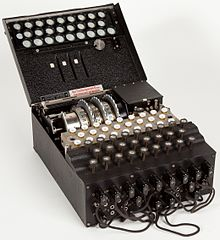
\includegraphics[width=40mm]{figures/enigma.jpg}
    \caption{\textit{Enigma I} reverse engineered by Marian Adam Rejewski}
    \label{fig:enigma}
\end{Figure}
\noindent

Today we are getting ever closer to reverse-engineering the cell.
The fields of synthetic and systems biology are beginning resemble engineering disciplines;
genetic engineering is becoming more precise, high-throughput in vitro experiments are performed
by robots and measurements of many desired observables can be obtained with high spatio-temporal resolution.
Advances in micro-fabrication \cite{Shafiee2017TissueMedicine} and in-vitro reconstitutive methods \cite{Gopfrich2018MasteringCells} have allowed biologists isolate pathways and mechanisms to a level of
mathematical and computational tractability \cite{Sharpe2017ComputerTomorrow.}. This section
outlines the scientific paradigms in these fields, their methods and limitations, and finally what this
thesis will attempt to contribute.

\section{Bottom-up and Top-down Biology}

Fortunately for biologists copies of the target of their reverse-engineering attempts are
available all around us. Less fortunate is the fact that most attempts at deconstructing
the cell end in loss of function and destruction of the individual components. This
restriction motivates system biologists to manipulate environmental signals \textit{in vivo}
and build mechanistic models from correlations between signals and responses \cite{Triantafillou2017PredictingCells}.
Models focus on relationships between macroscopic variables where the underlying
mechanisms are not known.
\\\\
\textit{In vitro} reconstitutive methods aim to isolate minimal mechanisms from the
complexity of the whole organism in order to unpick the relative importance of
microscopic details \cite{Gopfrich2018MasteringCells}.
In situations where purified proteins and crystal structures
are available these methods can quite accurately characterise the kinetics of
proteins. Relating these parameters to the \textit{in vivo} context however may
not be relevant, as too much of the complexity may have been stripped away. 
\\\\
From a theoretical modelling perspective, it is important to choose a time-scale
and space-scale that is relevant to the problem. If one is interested in tissue
dynamics, attempting to model DNA conformations within each cell will render the
problem intractable. As George Booth aptly put \textit{``most models are wrong but
some are useful"} so the role of theoretical descriptions in these settings is not
necessarily to describe the way reality \textit{is} but serve as tools to bridge
the non-intuitive gap between bottom-up and top-down approaches. Where intuition
fails is where the \textit{in silico} hypothesis testing playground becomes most
valuable \cite{Sharpe2017ComputerTomorrow.}.

\begin{Figure}
    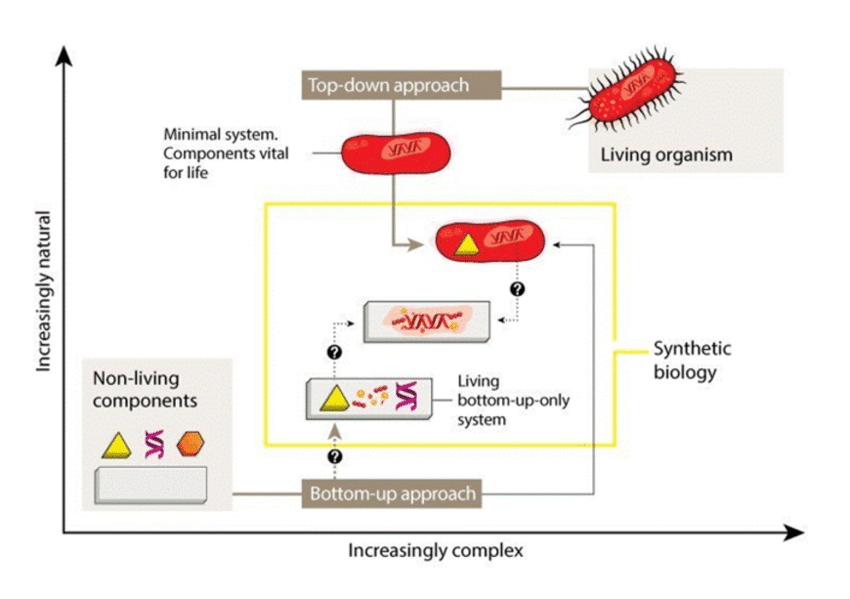
\includegraphics[width=80mm]{figures/top-down-bottom-up.png}
    \caption{Top-down and bottom-up modelling methods}
    \label{fig:tdbu}
\end{Figure}

\section{Design, Build, Test, Learn}
Systems and synthetic biology have historically made progress through a process
of brute force trial and error. This usually involves the interaction of many
custom-made parts that are iteratively optimised by human intervention. A trend
first observed in the 1980s known as \textit{Eroom's law} reveals that discoveries
in biotechnology are becoming slower and more expensive over time, despite
improvements in technology \cite{Scannell2012DiagnosingEfficiency}.
This problem is compounded by the ongoing reproduciblility crisis \cite{Ioannidis2005WhyFalse.}.
In the effort to transform methods used in academia and industry to become more
systematic and predictable, a standard for the Design--Build--Test--Learn cycle
has emerged -- showin in figure \ref{fig:dbtl}.
\\\\
This workflow has now been established as a paradigm with some aspects that have
been automated by liquid handling robots, bioreactor environments and image processing
pipelines. However, humans in the loop and custom moving parts still persist. The challenge
in automating these processes lies in defining a programming language that has a
sufficiently high level of abstraction for transparent implementation
while allowing for low-level customisation \cite{Abate2018ExperimentalSemantics}.

\begin{Figure}
    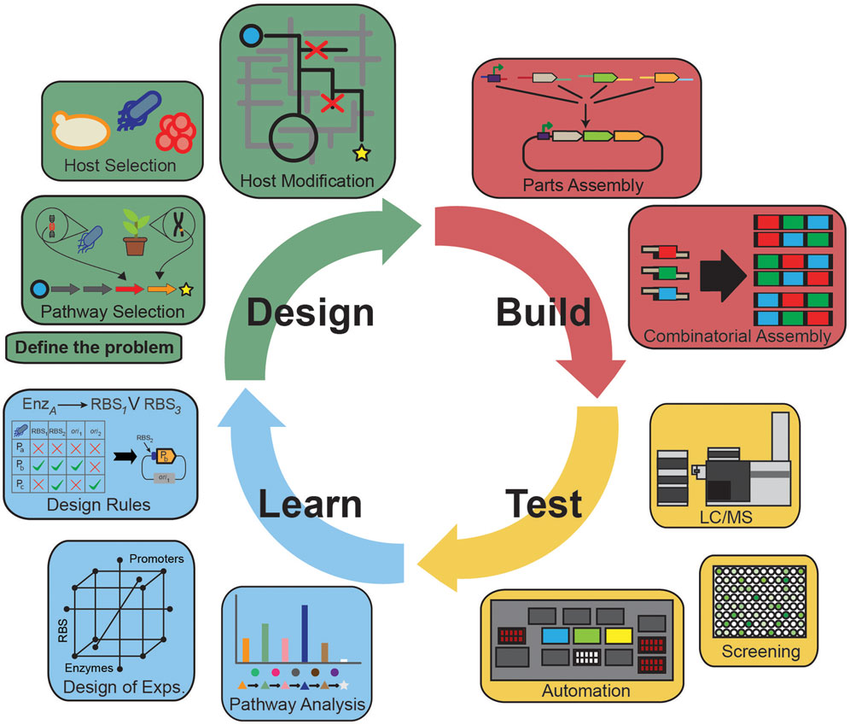
\includegraphics[width=60mm]{figures/dbtl.png}
    \caption{Design-Build-Test-Learn cycle from synthetic biology}
    \label{fig:dbtl}
\end{Figure}
\noindent
This thesis will focus on modelling and inference using systems of differential
and partial differential equations, which fits into the Design--Learn part of
the cycle. Differential equations occupy a small subset of possible modelling tools,
however they are amongst the most popular due to their ease of use formulation
and simulation. This ease of access creates a zoo of models in literature making
it difficult to identify the key ingredients that distinguish different models.
Furthermore the relationship between multiple plausible \textit{and} in-plausible hypotheses
is rarely investigated. This motivates desire for an automated Design--Learn pipeline --
outlined in Section \ref{section:design-learn} -- which can generate and catalogue models
in a transparent manner while producing insights for the Build stage.
This pipeline is applied in an experiment-theory collaboration described in
Chapter \ref{chapter:double-exclusive}.

\section{State of the Art}
\label{section:geometry}
\subsection{Inference of Differential Equations}
Following the initial literature on smooth and match estimators
\cite{Gugushvili2012Smoothing} -- which overcome the bottleneck
having to integrate a proposed hypothesis for every parameter update --
a plethora of methods for the inference of differential equations
became available \cite{Brunton2016SparseSINDYc,GorbachScalableSystems}.
The essence of these methods is to estimate the derivatives of the
data rather than integrate the model and simultaneously estimate 
the qualitative and quantitative behaviours. In most biological
experiments batch-to-batch variations decrease the certainty
with which it is possible to quantify a behaviour. Whether or not
a parameter is identifiable, reduntant or sloppy have become
key questions in biology \cite{Chis2016OnIdentifiability,
Gabor2017ParameterBiosystems,Villaverde2016StructuralModels}.

\subsection{Model Reduction and Classification}
Sloppiness and sensitivity anaylsis have been extensively used in the
search for reduced models. Linear
mappings between models that preserve stoichiometry and reactant structure were
investigated \cite{Cardelli2014MorphismsFunction,Cardelli2017MaximalSystems} and
computational tools based on partition-refinement were released
\cite{Cardelli2017ERODE:Equations}. Structural similarity between reaction
networks can be revealed by such mappings, elucidating the functional aspects of
complex networks in terms of simpler networks. The aim of the Design--Learn
pipeline is to extend this framework to nonlinear mappings with an emphasis on
geometry rather than kinetics. Most inference techniques attempt to match
geometry and kinetics simultaneously in an attempt to obtain a quantitative
model. This thesis emphasises that geometry alone should be prioritised in
order to obtain qualitatively equivalent models. Furthermore recent
results in pattern formation theory \cite{Halatek2018} do not depend
on kinetics at all, only geometry.

\section{Design--Learn Pipeline}
\label{section:design-learn}

This section outlines the proposal for a design--learn pipeline for
the purposes of model reduction and system design. Suppose experimental
collaborators have provided us with time-course gene expression data $\mathcal{D}$,
which could be taken via time-lapse microscopy of cells growing on microfluidic plates,
optical density measurements from microtiter plate assays or temporal snapshots of
flow cytometry measruements. On the other hand one may want to specify a behaviour
$\mathcal{H}$ which may have not yet been observed. This would be specified with
top-down constraints, i.e. there exist oscillations of a fixed frequency or
a region of bistability.

\subsection{Experimental Design Loop}
\label{section:experimental-design}

The experimentalists may want to know whether the data collected could
result in a model of predictive power without mechanistic knowledge
of the underlying biochemistry. Moreover it would be desirable gain insights
in parameter regimes in the vicinity of observations, without having to
wait for the theorists to produce a refined model. Such real-time insights
would guide data collection protocols, optimising the amount of information
gained while keeping the number of experiments performed to a minimum. Often
data is noisy and at worst case contradictory; these issues must also be exposed.

\begin{Figure}
    \begin{tikzpicture}[node distance=2cm]

        \node (nonparametric) [process, minimum width=5cm] {non-parametric inference};
        \node (data) [io, right of=nonparametric, xshift=1cm, yshift=2cm] {observations $\mathcal{D}$};

        \node (field) [decision, below of=nonparametric] {field $\Vector{f}$};
        \node (pred) [io, right of=field,  xshift=2cm] {predictions};

        \draw [arrow] (data) |- (nonparametric);
        \draw [arrow] (nonparametric) -- (field);
        
        \draw [arrow] (field) -- (pred);
        \draw [arrow,color=BurntOrange] (pred) -- +(0,3.5);

    \end{tikzpicture}
    \caption{Workflow loop for optimal experimental design, without mechanistic model}
    \label{fig:experimental-design}
\end{Figure}
\noindent
Figure \ref{fig:experimental-design} outlines the workflow for optimal experimental design.
The term \textit{non-parametric} defines the procedures that have prioritised  
functional generality and flexibility over mechanistic insights gained from the values
of the parameters and shapes of the mathematical forms. Neural networks and Gaussian process
regressors are examples of non-parametric estimation procedures, which produce an estimate
of the field $\Vector{f}$ that predicts gene expression rates at given expression levels.
Based on these predictions, the experimentalist may proceed to collect data in the most
informative parameter regions, which would in turn more accurately estimate $\Vector{f}$.

\subsection{Hypothesis Scoring and Model Refinement Loop}
\label{section:refinement}
Often predictions from field $\Vector{f}$ are not enough. Models constructed
with feasible biophysical assumptions $\Vector{h}(\Vector{\theta})$ have the potential
to extrapolate predictions and give concrete biophysical meanings to each parameter $\Vector{\theta}$.
This way the experimentalist knows exactly which modification to the system they must
make in order to achieve a desired behaviour. More often than not it is also unclear
whether the model and its assumptions are reasonable, which brings us to the desire
to score our hypotheses. For increased
accuracy and efficiency \cite{Meeds2019EfficientSystems} the mechanistic model
$\Vector{h}(\Vector{\theta})$ is inferred against non-parametric estimate $\Vector{f}$
rather than the data $\mathcal{D}$ directly. Furthermore as discussed in Section
\ref{section:geometry} the aim is to optimise geometry rather than kinetics.
Alternatively one may construct $\Vector{h}(\Vector{\theta})$ to cover a whole class
of models, such as those that satisfy mass-action. The expectation is that most of the
parameters would be zero but some would be informative. One can obtain a distribution
of optimal parameters $\rho(\Vector{\theta})$ by running multiple optimisations. From
this distribution one may construct alternative hypotheses and update $\Vector{h}(\Vector{\theta})$.
By iterating this procedure one would identify the minimal model within the model class that
explains the data. This process is known as model refinement or reduction.

\begin{Figure}
    \begin{tikzpicture}[node distance=2cm]

        \node (field) [decision] {field $\Vector{f}$};
        \node (hypothesis) [io, left of=field,  xshift=-2cm] {hypothesis $\Vector{h}(\Vector{\theta})$};
        \node (parametric) [process, below of=field, minimum width=5cm] {geometric inference};
        
        \node (params) [io, below of=parametric] {parameter distribution $\rho(\Vector{\theta})$};
        \node (score) [io, right of=params, xshift=4cm] {score};
        \node (decomp) [process, below of=params, minimum width=5cm] {clustering and decomposition};
        \node (models) [io, left of=decomp, xshift=-3cm] {models};

        \draw [arrow] (field) -- (parametric);
        \draw [arrow] (hypothesis) |- (parametric);
        \draw [arrow] (parametric) -- (params);
        
        \draw [arrow] (params) -- (decomp);
        \draw [arrow] (params) -- (score);
        \draw [arrow] (decomp) -- (models);
        \draw [arrow,color=ForestGreen] (models) -- +(0,5.5);

    \end{tikzpicture}
    \caption{Overview of hypothesis scoring pipeline and model refinement loop}
    \label{fig:non-parametric}
\end{Figure}

\subsection{System Design}
\label{section:system-design}
Suppose now that refined mechanistic models of the form $\Vector{h}(\Vector{\theta})$
have been obtained using the model refinement loop. These could be a library of known
parts that have been individually characterised, but never combined to form a larger
system. The experimentalists would like to create a system with a specified behaviour
$\mathcal{H}$ and would like to know which parts to combine and which modifications
to make. The model refinement loop can be used with the design as an input.

\begin{Figure}
    \begin{tikzpicture}[node distance=2cm]

        \node (nonparametric) [process, minimum width=5cm] {non-parametric inference};
        \node (design) [io, left of=nonparametric, xshift=-1cm, yshift=2cm] {design $\mathcal{H}$};

        \node (field) [decision, below of=nonparametric] {field $\Vector{f}$};
        \node (hypothesis) [io, left of=field,  xshift=-2cm] {models $\Vector{h}(\Vector{\theta})$};
        \node (parametric) [process, below of=field, minimum width=5cm] {geometric inference};
        
        \node (params) [io, below of=parametric] {parameter distribution $\rho(\Vector{\theta})$};

        \draw [arrow] (design) |- (nonparametric);
        \draw [arrow] (nonparametric) -- (field);
        
        \draw [arrow] (field) -- (parametric);
        \draw [arrow] (hypothesis) |- (parametric);
        \draw [arrow] (parametric) -- (params);

    \end{tikzpicture}
    \caption{Overview of system design pipeline}
    \label{fig:design}
\end{Figure}
\chapter{Theoretical Background}
\label{Introduction}
%
\epigraph{``\textit{You must understand, young Hobbit, it takes a long time to say anything in Old Entish. And we never say anything unless it is worth taking a long time to say.}"}{J.R.R. Tolkien}
%
This chapter presents a description of the two computational methods which have been primarily applied throughout the course of this thesis. Certain aspects of the thesis have required the use of other simulation methods, and these methods are outlined in the respective chapters.

\section{Molecular dynamics}\label{chapter:MD}
%
Molecular dynamics (MD) is a simulation method to study the dynamic evolution of a system of particles over time in accordance with their predefined interaction rules. For a macromolecular system, this is a powerful tool that is used to complement experiments to investigate the system to atomic resolution in space and \edit{femto}second resolution in time, to predict structural and thermodynamic properties such as free energies.\cite{mcquarrie1965statistical} The structural and thermodynamic behaviour can be compared to experimental data and provide insight to complex processes such as adsorption or ligand binding. An MD engine is a collection of numerical algorithms that defines a set of forces that act on all particles in a system, and iteratively evolves them along trajectories according to Newton's equations of motion.
%
\begin{equation} \label{eq:newtons2nd}
m_i \frac{\partial^2\mathbf{r}_i}{\partial t^2}=\mathbf{F}_i,\quad  i = 1,\,\dots,\,N
\end{equation}
%
Forces acting on particles $\mathbf{F}_i$ at positions $\mathbf{r}_i$ evolve the system to new positions according \edit{to} the potential energy function $U(\mathbf{r}_i$).
%
\begin{equation} \label{eq:newton}
\mathbf{F}_i = -\frac{\partial U}{\partial \mathbf{r}_i}
\end{equation}
%
In the case of biomolecular systems, the predefined interaction rules are a potential energy function (forcefield) which are requisite to calculating the forces. A forcefield maps the coordinates of the atoms $\mathbf{r}$ onto the potential energy surface as per the bonded and non-bonded energetic contributions of the macromolecular system components; namely the bonds, angles and dihedrals between atoms (bonded) and van der Waals and electrostatic (non-bonded) interactions.\cite{de2016role} A forcefield is usually expressed as sums of particle interactions and in the case of the \textit{optimised potentials for liquid simulations} (OPLS) forcefield \cite{jorgensen1988opls, jorgensen1996development} it takes the form expressed in (Eq.~\ref{eq:forcefield}), where ($K_b,\,K_{\theta},\,K_l,\,$) are respectively the bond, angle and dihedral force constants for each bonded interaction type and ($r_0,\, \theta_0,\, \phi_l$) are the equilibrium terms. The Lennard-Jones parameters ($\sigma_{ij}$,\, $\epsilon_{ij}$) that describe the interactions between types $i$ and $j$ are determined by taking a geometric average of the self-interaction parameters, i.e. ($(\sigma_{ii}\sigma_{jj})^{1/2}$). The final term in (Eq.~\ref{eq:forcefield}) is the Coulombic term that describes the energy between a pair of charges ($q_i,\,q_j$). 
%
\begin{equation} \label{eq:forcefield}
\begin{split}
U(\mathbf{r}) &= \sum_{bonds} K_b(r - r_0)^2 + \sum_{angles} K_{\theta}(\theta - \theta_0)^2 + \sum_{dihedrals} \, \, \sum_{l=1}^{4} \frac{K_{l}}{2}\left[1+(-1)^{l+1}\cos{(l\phi -\phi_{l})}\right] \\
&+ \sum_{nonbonded} 4\epsilon_{ij} \left[ \left( \frac{\sigma_{ij}}{r_{ij}}\right)^{12}-\,\,\left( \frac{\sigma_{ij}}{r_{ij}}\right)^{6} \right] + \sum_{i > j}  \frac{q_{i}q_{j}}{\edit{4 \pi \epsilon_{0}}r_{ij}}
\end{split}
\end{equation}
%
The principle of each bonded and non-bonded forcefield terms are illustrated in (Fig.~\ref{fig_ff}). Conventional potential energy functions describe a system with fixed charge for electrostatic interactions, electronic repulsion and dispersive non-bonded interactions through a van der Waals (Lennard-Jones) potential and bond stretching, bending and dihedral angle torsion potentials. More complex formulations of the potential energy function can include polarisation effects in polarisable forcefields,\cite{ponder2010current} or reactive forcefields that can account for bond order, bond formation and breaking.\cite{van2001reaxff}
%
\begin{figure}[H]
    \centering
    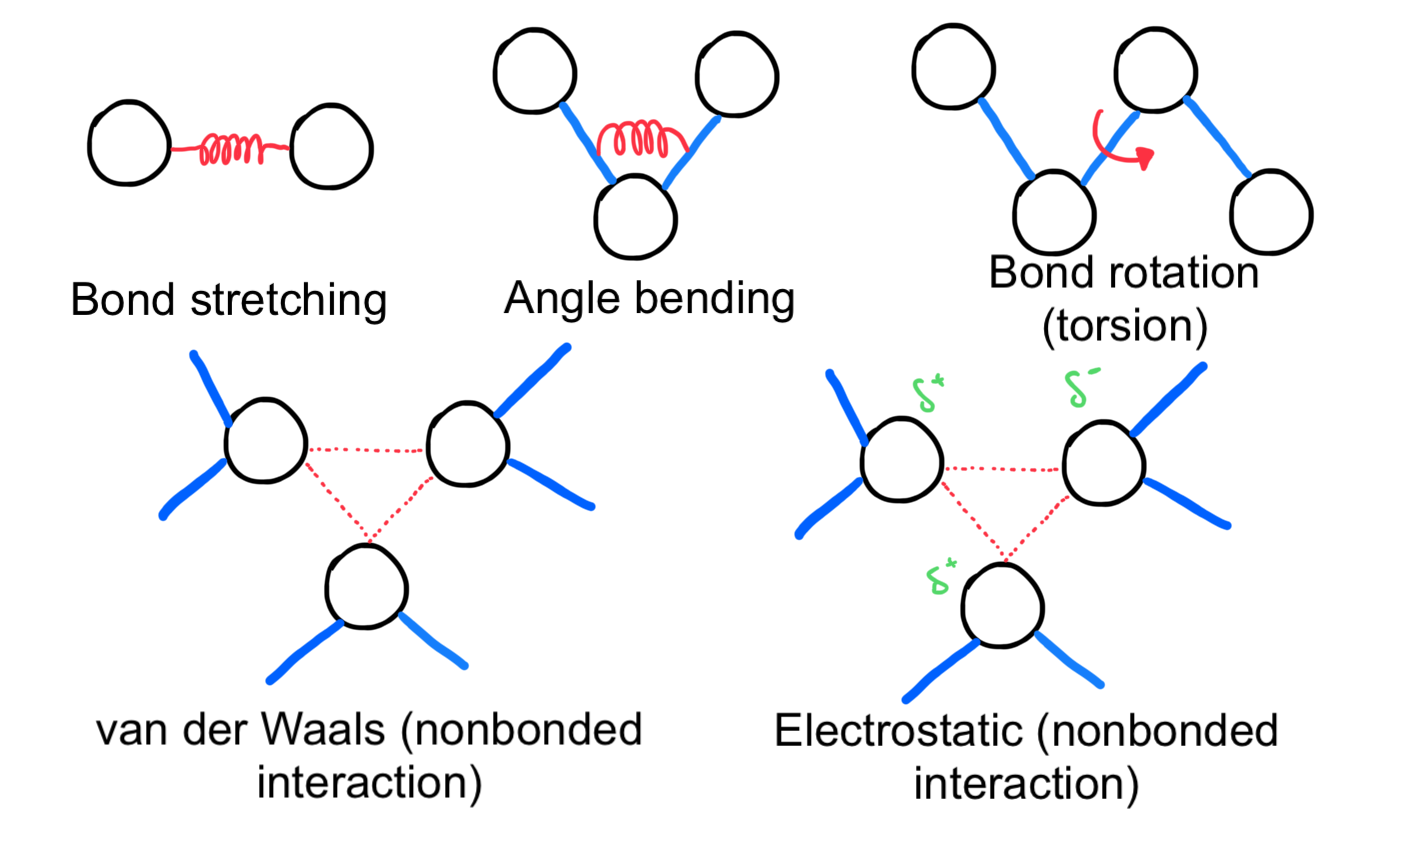
\includegraphics[width=0.99\columnwidth]{fig_ff.png}
    \caption{The energetic bonded and non-bonded components of a general biomolecular forcefield.}
    \label{fig_ff}
\end{figure}
%
The functional form of a forcefield (Eq.~\ref{eq:forcefield}) is composed of thousands of parameters for different types of atoms, bonds, bond angles, dihedral angles and nonbonded interactions.\cite{harder2016opls3} These parameters are typically derived semi-empirically through \textit{ab initio} quantum calculations on small molecules as well as optimising parameters to reproduce experimental properties of systems such as liquid densities and heats of vaporisation,\cite{vanommeslaeghe2010charmm} but retain the ability to accurately extrapolate to macromolecular properties such as the distribution of conformers such as $\phi,\, \psi$ angle distributions in proteins.\cite{mackerell2004improved} The transferability of forcefields is of course limited to the training and test sets, using them with an assumption of total coverage is erroneous, therefore special care is required when studying the dynamics of molecules with novel chemistries such as drug structures or exotic nanomaterials.\cite{harder2016opls3} One approach to derive the bespoke forcefield parameters from \textit{ab initio} quantum mechanical calculations is discussed in (\ref{sec:ddec}).
%
\subsection{Numerical integrators} \label{sec:integrators}
%
%\epigraph{``To do the same thing over and over again is not only boredom: it is to be controlled by rather than to control what you do."}{Heraclitus}
%
To solve \edit{the equations of motion (Eq.~\ref{eq:newtons2nd})} and translate the particle coordinates in the simulation system, one of many possible numerical integration methods is applied to approximate the exact solution to the differential equation. These methods generally start by replacing the derivative with a finite difference approximation of the form (Eq.~\ref{eq:finitediff}). 
%To solve a first order differential equation such as the one in (Eq.~\ref{eq:newton}) and translate the particle coordinates in the simulation system, one of many possible numerical integration methods is applied to approximate the exact solution to the differential equation. These methods generally start by replacing the derivative with a finite difference approximation of the form (Eq.~\ref{eq:finitediff}). 
%
\begin{equation} \label{eq:finitediff}
    \mathbf{r}'(t) \approx \frac{\mathbf{r}(t+\mathrm{d}t) - \mathbf{r}(t)}{\mathrm{d}t}
\end{equation}
This is rearranged to approximate new particle coordinates according to the force (Eq.~\ref{eq:newton}) and potential energy function (Eq.~\ref{eq:forcefield}), with respect to a discretised timestep $\mathrm{d}t$, this is known as the forward Euler algorithm (Eq.~\ref{eq:euler}).
%
\begin{subequations} \label{eq:euler}
%\begin{eqnarray}
\begin{align}
\begin{split}
    \mathbf{r}_i(t+\mathrm{d}t) &=  \mathbf{r}_i(t) +  \mathbf{v}_i(t)\mathrm{d}t
\end{split}\\
\begin{split}
    \mathbf{v}_i(t+\mathrm{d}t) &=  \mathbf{v}_i(t) + \frac{\mathbf{F}_i(\{\mathbf{r}_i(t)\})}{m_i}\mathrm{d}t
\end{split}
\end{align}
%\end{eqnarray}
\end{subequations}
%
This approach is first order convergent, meaning it has a local truncation error $\epsilon_{t+\mathrm{d}t}$ of order 2; namely the difference between the analytical ($\mathbf{r}(t+\mathrm{d}t)$) and approximated ($\mathbf{\tilde{r}}(t+\mathrm{d}t)$) solutions:
\begin{equation}
    \epsilon_{\,t+\dt} = \left|\mathbf{r}(t+\dt) - \mathbf{\tilde{r}}(t+\dt)\right|
\end{equation}
The analytical solution is expressed as a truncated Taylor series expansion:
\begin{equation}
    \mathbf{r}(t+\dt) = \mathbf{r}(t) + \mathbf{r'}(t)\dt + \frac{1}{2}\mathbf{r''}(t)\dt^2 %+ \frac{1}{6}\mathbf{r'''}(t)\dt^3
\end{equation}
Such that the truncated error of a single integration step using the forward Euler algorithm is given by:
\begin{subequations} \label{eq:euler_error}
%\begin{eqnarray}
\begin{align}
\begin{split}
    \epsilon_{\,t+\dt} &= \left|\mathbf{r}(t+\dt) - \mathbf{\tilde{r}}(t+\dt)\right|
\end{split}\\
\begin{split}
    &=  \left|\mathbf{r}(t) + \mathbf{r'}(t)\dt + \frac{1}{2}\mathbf{r''}(t)\dt^2 - \left[   \mathbf{r}(t) + \mathbf{v}(t)\dt   \right]\right|
\end{split}\\
\begin{split}
    &= \left| \frac{1}{2} \mathbf{r''}(t)\dt^2 \right| = \mathcal{O}(\dt^2)
\end{split}
\end{align}
%\end{eqnarray}
\end{subequations}
\vspace{-0.1cm}
As the integrator evolves the system coordinates iteratively, this error accumulates with respect to the size of the time step $\dt$, a scenario where the numerical solution converges to the analytical solution is therefore only possible in the limit of $\dt \rightarrow 0$, which is an impractical obstacle that would stand in the way of simulating meaningful (long enough) trajectories. The accumulation of errors results in the gradual change of the total energy of a closed system over time, an artefact known as energy drift. To accurately model the dynamics of a system at equilibrium, integrators are required to be symplectic, have time reversible symmetry and conserve linear momentum, angular momentum and energy. The forward Euler algorithm breaks both time-reversible symmetry i.e. whether the model is invariant to the substitution $\dt \rightarrow -\dt$, and symplectic condition i.e. that phase space volume is conserved. 

The leapfrog algorithm overcomes these limitations by performing a half velocity update step, followed by a full position update. New positions are used as initial conditions for computing a new set of atomic forces, combined with the final velocity half step this gives the velocity at the full step (Eq.~\ref{eq:froggy}).  
\begin{subequations} \label{eq:froggy}
%\begin{eqnarray}
\begin{align}
\begin{split}
\mathbf{v}_{i} \left(t + \frac{\dt}{2}\right) &= \textbf{v}_{i} (t) + \frac{\mathbf{F}_i(\{\mathbf{r}_i(t)\})}{m_i}\frac{\dt}{2} 
\end{split}\\
\begin{split}
\mathbf{r}_{i} (t + \dt) &= \mathbf{r}_{i} (t) + \mathbf{v}_{i} \left(t + \frac{\dt}{2}\right)\dt
\end{split}\\
\begin{split}
\mathbf{v}_{i} (t + \dt) &= \textbf{v}_{i} \left(t + \frac{\dt}{2}\right) + \frac{\mathbf{F}_i(\{\mathbf{r}_i(t+\dt)\})}{m_i}\frac{\dt}{2}
\end{split}
\end{align}
%\end{eqnarray}
\end{subequations}
The leapfrog algorithm is second order convergent and therefore has a local truncation error of order 3, following the same approach in (Eq.~\ref{eq:euler_error}):
\begin{subequations} \label{eq:froggy_error}
%\begin{eqnarray}
\begin{align}
\begin{split}
    \epsilon_{\,t+\dt} &= \left|\mathbf{r}(t+\dt) - \mathbf{\tilde{r}}(t+\dt)\right|
\end{split}\\
\begin{split}
    &= \left| \frac{1}{6} \mathbf{r'''}(t)\dt^3 \right| = \mathcal{O}(\dt^3)
\end{split}
\end{align}
\end{subequations}
The leapfrog algorithm (Eq.~\ref{eq:froggy}) meets the conditions outlined above and does not give rise to numerical artefacts for long simulation times as with the forward Euler algorithm. 

\subsection{Initial configuration} 
%
The investigation of a system's dynamics using an MD engine --- employing the algorithms covered in this chapter --- requires the user to identify molecular constituent atom types, atomic coordinates, the topology of the molecules of interest and their velocities. The input system structure is recognised by the employed forcefield to assign parameters in accordance with the functional form of the forcefield, generalised by (Eq.~\ref{eq:forcefield}). 

The user defined input coordinates of the system are paramount to correctly modelling the physical body under investigation; whether a protein, ligands or nanomaterials, it can be experimentally derived or inferred but requires pre-processing to ensure no experimental or modelling errors are present. Protein structures are available from X-Ray Diffraction (XRD) experiments, in the form of crystallographic 3-dimensional coordinate data hosted on the protein data bank (PDB) archive.\cite{PDB} A common experimental artefact from PDB structures is missing residues in the amino acid sequence, these are remedied using homology modelling. MODELLER is such a program, it performs comparative protein structure modelling by satisfaction of spatial restraints, filling in missing residues by aligning the input protein amino acid sequence to known related structures, producing 3-dimensional protein structures.\cite{marti2000comparative, webb2016comparative} 

In the case of small molecules such as ligands, widely available software packages can be utilised to define the input structure of molecules by hand using an interactive interface such as Avogadro.\cite{hanwell2012avogadro} Meanwhile, large non-organic materials can be generated by one of the many functionalities of the more complex initial configuration generators such as CHARMM-GUI; a web-hosted graphical user interface with an extensive set of tools ranging from nanomaterial, polymer and lipid membrane builders with multi-forcefield and multi-MD engine support.\cite{jo2008charmm,Lee2020} Another example of a versatile initial configuration builder is Packmol, it is a script-based and locally hosted software package that is widely used for generating complex systems.\cite{martinez2009packmol} Packmol affords user flexibility in ways interactive software may not, such as building the initial configuration of systems composed of different constituent molecules.

For entirely bespoke systems the molecular configuration is inferred through experimental techniques that do not accurately translate to 3-dimensional coordinates as is the case with proteins from the PDB. In particular, systems with exotic chemistries are not always readily prepared using the aforementioned initial configuration software, beside standardised protocol that may not reflect the accurate theoretical/phenomenological structure of the system in question. Such systems would require accuracy both in the distribution of atoms within the macromolecule as well as assigning the correct forcefield parameters. For example, some of the work in this thesis required the accurate characterisation of graphitic nanomaterials that required custom software to develop the macromolecular structures, topological properties and their corresponding forcefield parameters.\cite{albadri2020accurate-github} Custom software allows for flexibility in varying nanomaterial structural properties such as shape, size, chemical functionalisation and degree of functional group correlation. Software engineering custom software is an incredibly time consuming project, which is being accelerated by well executed and documented open source software initiatives.

\subsection{Periodic boundary conditions}
Periodic boundary conditions (PBC) are imposed on most MD simulation systems to approximate large systems that reside in a practically infinite environment, by construction. Simply put, particles leaving the unit cell in any of the ($\mathbf{x,y,z}$) directions reenter the unit cell from the opposing side in the respective dimension, retaining identical mechanical properties such as particle momenta. Particles in the unit cell interact with the particles in the closest neighbouring unit cell, restricted by the interaction cut-off radius as input by the user. As is common\edit{ly} the case and has been explained, the initial configuration can raise simulation artefacts and PBCs are no exception. A macromolecule such as a protein can self-interact through the boundary conditions, resulting in distorted dynamics if and when the simulation system is too small and the macromolecule isn't enveloped by sufficient explicit solvent molecules in all of the ($\mathbf{x,y,z}$) directions. The recommended protocol is that the simulation system should exceed twice the cut-off radius and have at least 1 nm of explicit solvent surrounding the macromolecule.\cite{deSouza1997} Charge interactions through PBCs could raise electrostatic artefacts, where a system without a neutral charge could sum to infinite charge through the periodic cells. Instead counter-ions are added to bring the simulation system to neutral charge, usually this sodium and chlorine ions for positive and negative charges, respectively. 

\subsection{Equilibration} \label{sec:equilibration}
The software used to create the initial configuration does not typically consider the energetics of the system, it is instead more suited to successfully geometrically organise a system's 3-dimensional molecular coordinates. As a result, these configurations may --- according to the initial configuration method --- exist in a high energy state, driven by anything from a high degree of atomic overlap to energetically unfavourable molecular conformations. Studying the system at equilibrium therefore requires a sequential treatment to bring the system's potential energy to a local minimum, followed by simulating trajectories to bring about thermal and barostatic equilibrium. These are known as the equilibration steps that precede the so called production-run which is used to gather the statistics for the desired system. 

\subsubsection{Energy minimisation}
To overcome the high energy of the initial configuration of the system, the MD engine employs the chosen forcefield to tweak the system coordinates until the energy corresponds to a local minimum in the potential energy surface through energy minimisation, instead of employing MD algorithms. A common approach to locate the local minimum of a multivariate and highly dimensional function that cannot be solved analytically is the gradient descent algorithm. A parameter (coordinate) vector ($\mathbf{r}$) is iteratively updated in the negative direction to the first order local gradient of the function ($\nabla \,V(\mathbf{r})$) being minimised in accordance with (Eq.~\ref{eq:gradient_descent}) until reaching convergence when the gradient is zero. The gradient is scaled by the step size ($\eta$), also known as the learning rate, the choice of which can impact whether the algorithm reaches convergence. Too small a step size could significantly retard the convergence, whereas a large step size could overshoot the local minimum parameter vector. 
%
\begin{equation} \label{eq:gradient_descent}
    \mathbf{r}_{n+1} = \mathbf{r}_{n} - \eta_{n} \, \nabla \, V(\mathbf{r}_{n})
\end{equation}
%
Tweaking the step size is therefore paramount to effectively or efficiently locate a local minimum; one such approach is a particular case of gradient descent known as the steepest descent algorithm, where the step size ($\eta$) is iteratively chosen to maximise the direction of the negative gradient of the function by minimising the objective function (Eq.~\ref{eq:obj_func}).\cite{Curry1944} 
%
\begin{equation} \label{eq:obj_func}
    \eta_n = \argmin_{\eta} \, \, V ( \mathbf{r}_{n} - \eta \, \nabla \, V(\mathbf{r}_{n})) 
\end{equation}
%
\subsubsection{Particle velocities}
To model the system in equilibrium, the system potential energy should oscillate close to its local minimum due to fluctuations in kinetic energy. Ensuring these oscillations in potential energy are stable and do not diverge due to large fluctuations, initial velocities are assigned to every particle in the system. There exist statistical constraints on the choice of particle velocities to ensure the system is in thermal equilibrium, namely that it abides by the equipartition theorem. To abide by this, all particles are randomly assigned a velocity from the Maxwell-Boltzmann distribution given by (Eq.~\ref{eq:Maxwell_distro}), where ($v$) is the velocity magnitude ($\sqrt{v_x^2 + v_y^2 + v_z^2}$) of the velocity vector ($\mathbf{v} = (v_x, v_y, v_z)$) and ($m$), ($T$) and ($k_B$) are the mass, desired temperature and the Boltzmann constant, respectively. 
%
\begin{equation} \label{eq:Maxwell_distro}
    f(v) = \frac{4}{\sqrt{\pi}} \left( \frac{m}{2k_B T} \right)^{3/2} v^2 \, \exp{\left( - \frac{mv^2}{2k_B T}\right)}
\end{equation}
%
Using this, the average square velocity is given by the integral:
\begin{equation}
    \langle v^2 \rangle = \int_0^{\infty} v^2 f(v)\,\mathrm{d}v = \frac{3k_B T}{m}
\end{equation}
%
%\subsection{Constraint algorithms}
%The application of numerical integrators as discussed in section (\ref{sec:integrators}) can be made more efficient by extending the rate of integration (update step) in (Eq.~\ref{eq:froggy}) without encroaching on the time-frequency of the fastest dynamics in the simulation system. It turns out that the highest frequency dynamics in any biomolecular system is the bond frequency of the 
%\subsubsection{LINCS}

\subsection{Thermostats}
%
%\epigraph{``The worst thing you can do about a situation is nothing."}{Ice Cube}
%
Performing iterative integration of Newton's equations of motion (Eq.~\ref{eq:newton}) in this way generates a microcanonical ensemble where the simulation system's number of atoms ($N$), volume ($V$) and total energy ($E$) are kept constant. With conserved energy, the system is in a steady state that does not evolve over time, despite all its constituent parts being in motion. The microcanonical ($NVE$) ensemble assigns equal probability to all the system microstates within this energy $E$, all microstates outside this range have zero probability and are never sampled in an equilibrium configuration. The alternative approach is to model the system in a canonical ($NVT$) ensemble, where the system no longer has conserved energy but the average temperature ($T$) is kept constant. By allowing the simulation system to exchange energy with its environment --- implemented through coupling to a heat reservoir --- it is able to explore a phase space that includes microstates with different energies.\cite{ford2013statistical} In order to implement the canonical ensemble in MD simulations, in which temperature is conserved instead of energy, the integration of Newton's equations of motion have to be coupled to a thermostat. 

A thermostat is an algorithm that introduces a fictitious dynamical variable, which slows down or accelerates particles until the temperature is equal to the desired value through coupling to an external heat bath. One of the simplest implementations of a thermostat is the Berendsen thermostat which rescales the velocities of all particles at each integrator timestep with a nonphysical force (Eq.~\ref{eq:berendsen}) with a scale factor ($\lambda$) to control the total mean kinetic energy.\cite{berendsen1984molecular} 
%
\begin{equation} \label{eq:berendsen}
    \lambda\,(t) = \left[    1 + \frac{\dt}{\tau_{\,T}} \left( \frac{T_0}{T(t-\frac{1}{2}\dt) - 1}   \right) \right]^{1/2}
\end{equation}
%
$\tau$ is a time constant related to the temperature coupling time constant $\tau_T$ by $\tau = 2C_V \tau_T / N_{df}k_B$, where $C_V$ is the total heat capacity of the system, $N_{df}$ the numer of degrees of freedom in the system and $k_B$ is the Boltzmann constant. Deviations of the simulation system temperature $T_0$ are corrected to the target temperature $T$ according to:
\begin{equation} \label{eq:berendsen_rate}
    \frac{\mathrm{d}T}{\dt}  = \frac{T_0 - T}{\tau}
\end{equation}
%
The system kinetic energy ($K$) is scaled with $\lambda$ (Eq.~\ref{eq:berendsen}) at each integrator step through:
\begin{equation} \label{eq:berendsen_kinetic}
    \Delta\, K = (\lambda - 1)^2\, K
\end{equation}

By design (see \ref{sec:equilibration}) the particle velocities are distributed according to the Maxwell-Boltzmann function. Scaling the kinetic energy with the Berendsen thermostat (Eq.~\ref{eq:berendsen_kinetic}) suppresses the fluctuations in kinetic energy and particle velocities no longer adopt a Maxwell-Boltzmann distribution. This means that the Berendsen thermostat does not generate a canonical ensemble and will give rise to artefacts and incorrect sampling of the system's phase space. A particular manifestation within a system is that the total kinetic energy is not shared equally among all kinetic degrees of freedom --- hence violating the theory of equipartition --- where the kinetic energy instead flows from higher energy degrees of freedom to translational and rotational degrees of freedom. This results in a part of the system freezing into a single conformation and travelling through the simulation box with high momentum, this is known as the flying ice cube effect.\cite{harvey1998flying} 

To remedy this artefact, a stochastic term ($\mathrm{d}W$) in the form of a Wiener process is added to the Berendsen thermostat (Eq.~\ref{eq:berendsen}) that ensures the correct kinetic energy distribution and that the resulting dynamics produce a correct canonical ensemble.
%
\begin{equation} \label{eq:bussi_thermostat}
    \mathrm{d}K = (K_0 - K)\frac{\dt}{\tau_{\,T}} + 2 \sqrt{\frac{K\,K_0}{N_{df}}} \frac{\mathrm{d}W}{\sqrt{\tau_{\,T}}}
\end{equation}
This is known as the Bussi–Donadio–Parrinello thermostat (Eq.~\ref{eq:bussi_thermostat}).\cite{bussi2007canonical}
\subsection{Barostats}
In a similar fashion, an isothermal-isobaric ($NPT$) ensemble can be generated by a rigorous barostat algorithm by coupling the system to a pressure bath. One approach that successfully generates an isothermal-isobaric ensemble is the Parinello-Rahman barostat.\cite{parrinello1981polymorphic} This approach is implemented through coupling the imbalance between the simulation system pressure and the external (bath) tensorial pressure field to changes in the shape and size of the simulation box. The simulation box vectors are represented by the matrix ($\mathbf{b}$) and obey the equation of motion in (Eq.~\ref{eq:PR_EoM}), defined with respect to the simulation box volume ($V$), coupling strength matrix ($\mathbf{W}$), system pressure ($\mathbf{P}$) and reference pressure ($\mathbf{P}_{ref}$).
%
\begin{equation} \label{eq:PR_EoM}
    \frac{\mathrm{d}\mathbf{b}^2}{\dt} = V \mathbf{W^{-1}}\mathbf{b'}^{-1} (\mathbf{P}-\mathbf{P}_{ref})
\end{equation}
%
The system pressure tensor ($\mathbf{P}$) is calculated from the difference in kinetic energy ($\mathbf{K}$) and the virial tensors (Eq.~\ref{eq:virial}), where ($\otimes$) denotes the tensor product. 
%The scalar pressure is calculated from the pressure tensor through $P = \mathrm{Tr}(\mathbf{P})/3$. 
%
\begin{subequations} \label{eq:virial}
%\begin{eqnarray}
\begin{align}
\begin{split}
    \mathbf{P} = \frac{2}{V}(\mathbf{K} - \Xi)
\end{split}\\
\begin{split}
    \mathbf{K} = \frac{1}{2}\sum_i m_i \mathbf{v}_i \otimes \mathbf{v}_i
\end{split}\\
\begin{split}
    \Xi = -\frac{1}{2}\sum_{i<j} \mathbf{r}_{ij} \otimes \mathbf{F}_{ij} 
\end{split}
\end{align}
\end{subequations}
% if you want derivations and more special cases (PBC) see https://cfwebprod.sandia.gov/cfdocs/CompResearch/docs/JCPSA613115154107_1.pdf
%
The coupling strength matrix ($\mathbf{W}$) is defined with respect to the isothermal compressibility ($\beta_{ij}$), pressure time constant ($\tau_P$) and the largest box matrix element ($L$) as $(\mathbf{W}^{-1})_{ij} = 4 \pi^2 \beta_{ij} / 3 \tau_P^2 L$. Since the implementation of pressure coupling requires a change in both simulation box vector and particle equations of motion, a modification is applied to the system Hamiltonian, where the modified Hamiltonian ($\mathcal{H}_{PR}$) is given by (Eq.~\ref{eq:PR_hamil}), where ($U$) and ($K$) denote the potential and kinetic energies, respectively. 

\begin{equation} \label{eq:PR_hamil}
    \mathcal{H}_{PR} = U + K + \sum_i P_{ii} V + \sum_{ij} \frac{1}{2} W_{ij} \left(\frac{\mathrm{d}\,b_{ij}}{\dt}\right)^2
\end{equation}

The equations of motion of the system's particles are given by (Eq.~\ref{eq:PR_motion}), where the added term takes the form of a friction term. It is however fictitious and solely there to define the particle equations of motion with respect to the simulation box vectors through the term.

\begin{subequations} \label{eq:PR_motion}
%\begin{eqnarray}
\begin{align}
\begin{split}
    \frac{\mathrm{d}^2 \mathbf{r}_i}{\dt^2} = \frac{\mathbf{F}_i}{m_i} - \Lambda \frac{\mathrm{d} \mathbf{r}_i}{\dt}
\end{split}\\
\begin{split}
    \Lambda = \mathbf{b}^{-1} \left[  \mathbf{b} \frac{\mathrm{d}\mathbf{b'}}{\dt} + \frac{\mathrm{d}\mathbf{b}}{\dt} \mathbf{b'} \right] \mathbf{b'}^{-1}
\end{split}
\end{align}
\end{subequations}
%
\subsection{Parallelisation}
Simulating the dynamics of biomolecular systems requires a large system size to answer questions of meaningful scientific interest. The computational cost of running MD algorithms scales with the number of particles in the simulation system, therefore the implementation of MD algorithms in parallelised standards is necessary. Accelerating MD simulations is achieved by both parallelised standards where the software code is written to specify how tasks are divided between computational resources, and by implementing methods that reduce the complexity of particularly costly calculations involved in MD algorithms, e.g. evaluating a list of distances between particles and calculating long-range interactions. 

\subsubsection{Domain decomposition}
The naive approach of calculating the distances between particle coordinates in the simulation system is through a brute-force algorithm, where the distances are computed between all ($N(N-1)/2$) point pairs and the smallest distance pair is picked. The list of distances is used to evaluate the interaction type and its magnitude, thus its contribution to the total system energy at that point in the simulation. Performing this by brute force requires $\mathcal{O} (N^2)$ time. An alternative approach to calculating particle pair-wise distances and their interactions is known as domain decomposition, in which a data structure is implemented where distances are evaluated only within a predefined cut-off distance, therefore reducing the $\mathcal{O} (N^2)$ time complexity of the closest pair of points problem. The cut-off distance is generally the distance within which short-range non-bonded interactions are present. This data structure works by decomposing the 3-dimensional simulation domain into cells with a edge length equal to or greater than the interaction cut off distance, where pairwise distances are now computed for particles between neighbouring cells instead of the entire simulation domain. For a 3-dimensional simulation domain, a 3-dimensional cell has 26 neighbouring cells for which pairwise distances need to be calculated. The computational time complexity of this operation is reduced from $\mathcal{O} (N^2)$ to $\mathcal{O} (N\overline{c}) \in \mathcal{O} (N)$, where $\overline{c}$ denotes the average number of particles per cell ($N/m$), where ($m$) is the number of cells decomposing the domain. 

\subsubsection{Particle-mesh-Ewald summation} \label{sec:pme}
Having reduced the cost of evaluating particle pairwise distances for short-range interactions does not solve the problem of computing pairwise distances to calculate long range non-bonded interactions, such as electrostatics and the Lennard-Jones dispersion ($1/r^6$) term in (Eq.~\ref{eq:forcefield}). Ewald summation \cite{ewald1921berechnung} was introduced for the treatment of such long-range interactions, however it scales as ($\mathcal{O}(N^2)$) in time which is impractical for the treatment of large simulation systems. However it does form the foundations of methods such as particle-mesh-Ewald (PME) \cite{Darden1993} which scales as ($\mathcal{O}(N\,\log\,N)$) in time.

Within Ewald summation formalism, the total electrostatic energy for $N$ particles for a unit cell --- defined with respect to periodic images at positions ($\mathbf{r}_j + \mathbf{n}$) --- is represented by (Eq.~\ref{eq:ewald_unit_cell}), where ($\mathbf{n} =  n_1\mathbf{a}_1 + n_2\mathbf{a}_2 + n_3\mathbf{a}_3$) are the box index vectors and the ($\sum_{n}^{\ast}$) sum indicates that terms with ($i=j$) and ($\mathbf{n} = 0$) should be omitted. 
%
\begin{equation} \label{eq:ewald_unit_cell}
E(\mathbf{r}) = \frac{1}{2}\sum_{n}^{\ast}\sum_{i} \sum_{j} \frac{q_i q_j}{{\left| \mathbf{r}_j - \mathbf{r}_i + \mathbf{n} \right| }}
\end{equation}
%
The expression is a slowly converging sum that can be converted to quickly converging expressions for short-range ($E_{sr}$) and long-range ($E_{lr}$) electrostatic interactions and a self-interaction correction term ($E_{corr}$); long-range interactions are computed in reciprocal space through the use of Fourier transforms. \cite{ewald1921berechnung, Essmann1995}
%
\begin{subequations} \label{eq:ewald_sep}
\begin{align}
\begin{split}
E = E_{sr} + E_{lr} + E_{corr} 
\end{split}\\
\begin{split} \label{eq:ewald_sr}
E_{sr} = \frac{1}{2} \sum_{n}^{\ast} \sum_{i,j}^{N}  q_i q_j \frac{\mbox{erfc}\left(\beta \left| \mathbf{r}_j - \mathbf{r}_i + \mathbf{n} \right|\right)}{\left| \mathbf{r}_j - \mathbf{r}_i + \mathbf{n} \right|}
\end{split}\\
\begin{split} \label{eq:ewald_lr}
E_{lr} = \frac{1}{2 \pi V} \sum_{\mathbf{m} \neq 0} \frac{ \exp{(- \pi^2 \mathbf{m}^2 / \beta^2)}}{\mathbf{m}^2} S(\mathbf{m}) S(-\mathbf{m})
\end{split}\\
\begin{split} \label{eq:ewald_corr}
E_{corr}=-\frac{1}{2} \sum_{(i, j) \in M} \frac{q_{i} q_{j} \operatorname{erf}\left(\beta\left|\mathbf{r}_{i}-\mathbf{r}_{j}\right|\right)}{\left|\mathbf{r}_{i}-\mathbf{r}_{j}\right|}-\frac{\beta}{\sqrt{\pi}} \sum_{i}^{N} q_{i}^{2}
\end{split}
\end{align}
\end{subequations}
%
In (Eq.~\ref{eq:ewald_lr}), the volume of the unit cell ($V$) is given by ($\mathbf{a}_1 \cdot \mathbf{a}_2 \times \mathbf{a}_3$), ($\mathbf{m}$) denotes the reciprocal lattice space vectors ($\mathbf{m}  =  m_1\mathbf{a}_1^{\ast} + m_2\mathbf{a}_2^{\ast} + m_3\mathbf{a}_3^{\ast}$) and ($S(\mathbf{m}) = \sum_{j}^{N} q_j \exp{(2 \pi i\, \mathbf{m\cdot r})}$) is the structure factor. The error function ($\mathrm{erf}(x)$) in (Eq.~\ref{eq:ewald_corr}) is related to the complementary error function in (Eq.~\ref{eq:ewald_sr}) by ($1 - \mathrm{erfc}(x)$). The ($\beta$) parameter in (Eq.~\ref{eq:ewald_sep}) determines the relative weight of the direct and reciprocal sums and can be used to control the rates of convergence of the respective terms. Algorithmic optimisation of the ($\beta$) parameter can reduce the time complexity of Ewald summation from ($\mathcal{O}(N^2)$) to ($\mathcal{O}(N^{3/2})$).\cite{karasawa1989acceleration,Darden1993} 

The PME method also separates the short- and long-range interactions, similarly to the Ewald method in (Eq.~\ref{eq:ewald_sep}), where short-range and long-range interactions are evaluated in real and reciprocal space, respectively. The real space (short-range) sum has a time complexity of ($\mathcal{O}(N)$) by virtue of the pairwise minimum distance computation from domain decomposition, leaving the reciprocal space sum (Eq.~\ref{eq:ewald_lr}) as the bottleneck. The treatment of the long-range non-bonded interactions is accelerated to ($\mathcal{O}(N \log N)$) time complexity by assigning the charges ($q$) to a discrete grid (mesh) using cardinal B-spline interpolation, \cite{Essmann1995} resulting in a charge density field. The charge density field is defined on a discrete lattice in real space and is Fourier transformed to reciprocal space, enabling the long-range interaction term to be evaluated using a single sum over the grid in reciprocal ($\mathbf{k}$) space (Eq.~\ref{eq:pme}), where ($\tilde{\Phi}_{lr}(\mathbf{k})$) denotes the Fourier transformed potential from Ewald summation --- implicit in (Eq.~\ref{eq:ewald_lr}) --- and $\tilde{\rho}(\mathbf{k})$ the Fourier transformed charge density field.
%
\begin{equation} \label{eq:pme}
    E_{lr} = \sum_{\mathbf{k}} \tilde{\Phi}_{lr}(\mathbf{k}) \left| \tilde{\rho}(\mathbf{k})\right|^2  
\end{equation}
%
%
%\edit{Should I say something about how they're computationally implemented and how that helps with the parallelisation of MD algorithms, in line with the name of this chapter? --- CDL I think that would be nice}
%
%The evolution of high performance computing scale and their different architectures have had a big impact on the acceleration of MD simulations in recent decades, most notably the transferability between graphical processing unit (GPU) architecture and MD spatial domains. \edit{You would have to say more about this... cite implementation paper of gmx 2020 where all bonded and non-bonded interactions happen on GPU.} Other more bespoke architectures designed particularly for solving MD algorithms are at the cutting edge; simulating larger systems in a relatively short time. \edit{ANTON is ...} 
%\subsubsection{Domain decomposition}
%Within computational processing unit (CPU) parallelisation, a simulation system is divided by the number of CPU threads, such that --- at least in principle --- $N$ threads accelerate the simulation by $N$ times. Decomposing the simulation system into cells with respect to its coordinate Cartesian space by the available number of CPU threads is known as domain decomposition. In domain decomposition, integration algorithms are performed independently on each thread, while memory of neighbouring cells and their containing particles is maintained.
% ---------------------
%
%       DFT INTRO
%
% ---------------------
%\newpage
\section{Density Functional Theory} \label{chapter:onetep}
So far the discussion of molecular dynamics has considered the energetics and the calculation of forces on individual atoms in a macromolecular system, using Newton's  laws of motion in classical mechanics (Eq.~\ref{eq:newtons2nd}). The computation of energies and forces in classical MD is hinged on the validity of a forcefield that is derived from both \textit{ab initio} and phenomenological approaches. \textit{Ab initio} quantum mechanical approaches such as density functional theory (DFT) calculate the electronic ground state of a molecular system using the Schr\"odinger equation (Eq.~\ref{eq:schrodinger}) as a basis for its framework, which involves the treatment of both electrons and nuclei. Within the Schr\"odinger equation, the Hamiltonian operator ($\mathcal{H}$) acts on the quantum mechanical system; formulated in terms of the many electron wave function ($\Psi$).\cite{Schrodinger1926undulatory}
%
\begin{equation} \label{eq:schrodinger}
    \mathcal{\hat{H}}\, | \Psi \rangle = E \, | \Psi \rangle
\end{equation}
%
Solving the Schr\"odinger equation for a many electron system is an intractable and impossible problem to solve analytically, due to the correlated motion of electrons described by the many electron wave function ($\Psi$), containing $3N$ degrees of freedom, where $N$ is the number of electrons in question. DFT reformulates the Schr\"odinger equation from a single $N$-body problem to $N$ single-body problems.

Instead of the wave function, DFT solves the electronic Hamiltonian (Eq.~\ref{eq:molhamil}) by considering the density of the electrons in a system as a fundamental variable. It is expressed with respect to the kinetic energy operators for each electron ($\hat{T}_e$) and nucleus ($\hat{T}_e$) in the system, as well as the potential energy operators between the electrons and nuclei ($\hat{V}_{ne}$), electron-electron repulsion ($\hat{V}_{ee}$) and nuclei-nuclei repulsion ($\hat{V}_{nn}$). 
%
\begin{equation} \label{eq:molhamil}
\begin{split}
\hat{\mathcal{H}}  &=  \hat{T}_e + \hat{V}_{ne} + \hat{V}_{ee} + \hat{T}_{n} + \hat{V}_{nn}
\\ &= - \frac{\hbar}{2m} \sum_{i}^{N} \nabla_i - e^2 \sum_{I=1}^{N} \sum_{i=1}^{N} \frac{Z_I}{|\mathbf{R_I - r_i}|}  + \frac{e^2}{2} \sum_{i \neq j}^{N} \sum_{j \neq i}^{N} \frac{1}{|\mathbf{r_i - r_j}|} - \frac{\hbar^2}{2} \sum_{I=1}^{P} \frac{\nabla_i^2}{M_I} \\
& \quad + \frac{e^2}{2} \sum_{I=1}^{P} \sum_{J \neq I}^{P} \frac{Z_I Z_J}{|\mathbf{R_I - R_J}|}
\end{split}
\end{equation} 
%
The reformulation from wave functions to the density of electrons is based on Hohenberg-Kohn theorem and the Kohn-Sham equations. Fermi and Thomas first proposed this idea and derived a differential equation for the density,\cite{Thomas1927, fermi1927metodo} therefore negating the need to work in terms of the one-electron orbital. It later required the work of Hohenberg and Kohn to formulate the theory on a strong mathematical basis,\cite{hohkohn} giving rise to the Hohenberg-Kohn theorem. The theory was further developed with the Kohn-Sham framework,\cite{kohnsham} where the problem of interacting electrons in a static external potential is reduced to non-interacting electrons moving in an effective potential. 
%
The Born-Oppenheimer approximation makes solving the Schr\"odinger equation easier by imposing the separation of nuclear and electronic motion to the wave function ($\Psi(\mathbf{r}, \mathbf{R})$).\cite{BO} This is justified by the difference in momentum of the nuclei compared to electrons, where the much heavier nucle\edit{i} must therefore have minuscule velocities. 
%
\begin{equation} \label{eq:BO}
\Psi(\mathbf{r}, \mathbf{R}) = \psi(\mathbf{r}, \mathbf{R}) \phi(\mathbf{R})
\end{equation}
%
\subsection{Hohenberg-Kohn Theorems}
%
The Hohenberg-Kohn theorems are the basis for computing the ground state properties of a system without directly dealing with the highly dimensional many-electron wave function. It instead reformulates the problem in terms of the electronic density and treats the system of electrons moving under the influence of an external potential, which encompasses all effects external to the electrons themselves such as Coulombic effects from atomic nuclei. As such, and due to the separation of nuclear and electronic motion via the Born-Oppenheimer approximation, the repulsive Coulombic potential between nuclei can be treated separately as an external potential:
%
\begin{equation}
V_{\mathrm{ext}}(\mathbf{r})=-\sum_{I} \frac{Z_{I}}{\left|\mathbf{r}_I-\mathbf{r}_i\right|}
\end{equation}
%
Therefore the entire electronic Hamiltonian (Eq.~\ref{eq:molhamil}) can be expressed as ($\hat{H} = \hat{F} + \hat{V}_{\mathrm{ext}}$), where ($\hat{F}$) is given by (Eq.~\ref{eq:hohkohn_F}) and the external potential operator is given by the sum of external potentials ($\hat{V}_{\mathrm{ext}} = \sum_i V_{\mathrm{ext}} (\mathbf{r}_i)$).
%
\begin{equation} \label{eq:hohkohn_F}
\hat{F}=-\frac{1}{2} \sum_{i} \nabla_{i}^{2}+\frac{1}{2} \sum_{i} \sum_{j \neq i} \frac{1}{\left|\mathbf{r}_{i}-\mathbf{r}_{j}\right|} = \hat{T}_e + \hat{V}_{ee}
\end{equation}
%
The expression for ($\hat{F}$) is universal to all systems consisting of $N$ electrons, meaning that the external potential ($V_{\mathrm{ext}}$) and the number of electrons in a given system ($N$) completely control ($\hat{H}$) and the ground state wave function ($\Psi_0$). The ground state wave function and the Hamiltonian give rise to the ground state density ($n(\mathbf{r}$):
%
\begin{equation} \label{density}
n(\mathbf{r}) = \int \prod_{i=2}^{N} | \Psi_0 (\mathbf{r, r_2, r_3, \dots, r_N)}|^2 \mathrm{d} \mathbf{r}_i = \langle \Psi_0 | \hat{n} |\Psi_0 \rangle
\end{equation} 
%
Given this, the electronic density ($n(\mathbf{r})$) and the ground state wave function ($\Psi_0$) are functionals (a function of a function) of the number of electrons ($N$) and the external potential ($V_{\mathrm{ext}}$). 
 
The first Hohenberg-Kohn theorem states that the external potential ($V_{\mathrm{ext}}(\mathbf{r})$) is a unique functional of the ground state electronic density ($n(\mathbf{r})$), therefore the total energy is also a functional of the ground state electronic energy. Indeed, it turns out a consequence of this theorem is that all system properties can be determined just by the electronic ground state density.\cite{hohkohn} 

The proof for this theorem is a simple \textit{reductio ad absurdum} argument. Consider a many-electron Hamiltonian of the form ($H = T + V$) and a different Hamiltonian ($H' = T + V'$), with wave functions ($\Psi$) and ($\Psi '$) respectively and where ($V - V' \neq \mathrm{constant}$). The electron density is defined by (Eq.~\ref{density}) and we assume that the electron density is equal for ($V$) and ($V'$). 
%
According to the Rayleigh-Ritz variational theorem, the ground state energy satisfies the inequality (Eq.~\ref{ritz}).
%
\begin{subequations} \label{ritz}
\begin{align}
\begin{split}
E_0 < \langle \Psi'|H|\Psi'\rangle &= \langle \Psi'|H'|\Psi'\rangle + \langle \Psi'|H-H'|\Psi'\rangle
\end{split}\\
\begin{split}
&= E_0 ' + \int n(\mathbf{r}) (V(\mathbf{r}) - V'(\mathbf{r})) d \mathbf{r}
\end{split}
\end{align}
\end{subequations}
%
The inequality refers to different Hamiltonians, therefore the eigenstates ($\Psi$) and ($\Psi '$) are different. By swapping the primed and unprimed quantities in (Eq.~\ref{ritz}) we get the expression (Eq.~\ref{ritz2}).
%
\begin{subequations} \label{ritz2}
\begin{align}
\begin{split}
E_0' < \langle \Psi|H'|\Psi\rangle &= \langle \Psi|H|\Psi\rangle + \langle \Psi'|H'-H|\Psi'\rangle
\end{split}\\
\begin{split}
&= E_0 + \int n(\mathbf{r}) (V'(\mathbf{r}) - V(\mathbf{r})) d \mathbf{r}
\end{split}
\end{align}
\end{subequations}
%
Summing (Eq.~\ref{ritz}) and (Eq.~\ref{ritz2}) together results in an absurd statement, namely that ($E_0 + E_0 ' < E_0' + E_0$), consequently two potentials ($V$) and ($V'$) can correspond to the same electron density, which is proven not to be the case. Hence, ($V'(\mathbf{r}) \neq V(\mathbf{r})$) for a given ($n(\mathbf{r})$).
%

The second Hohenberg-Kohn theorem is that the total energy of a system --- a functional of the ground state electronic density as by the first Hohenberg-Kohn theorem --- is minimised to arrive at the correct ground state energy. Regardless of the external potential of a system ($V_{\mathrm{ext}}$), the functional to be minimised is universal for any system and is given by:
\begin{equation} \label{func}
E[n(\mathbf{r})] = F[n(\mathbf{r})] + \int n(\mathbf{r}) V_{\mathrm{ext}}(\mathbf{r}) \mathrm{d} \mathbf{r}
\end{equation}
where, as outlined in (Eq.~\ref{eq:hohkohn_F}), the electronic energies are contained within the universal functional ($F[n(\mathbf{r})]$). The total energy functional (Eq.~\ref{func}) is equivalent to the ground state energy, given by the expectation value with respect to the ground state wave function:
%
\begin{equation}
    E = E[n] = \langle \Psi_0 | \hat{H} | \Psi_0 \rangle
\end{equation}
%
To show this, consider an electronic density ($n'(\mathbf{r})$) different to the ground state electronic density ($n(\mathbf{r})$) has a different wave function ($\Psi'$). The energy corresponding to this state ($E'$) has a higher energy than the ground state energy ($E$), according to the variational theorem as seen in (Eq.~\ref{ritz}):
%
\begin{equation}
    E = \langle \Psi_0 | \hat{H} | \Psi_0 \rangle > \langle \Psi ' | \hat{H} | \Psi ' \rangle = E'
\end{equation}
Given this, the total energy functional (Eq.~\ref{func}) gives the exact ground state energy ($E$) only for the exact ground state electronic density ($n(\mathbf{r})$). However, the difficulty is that ($F[n(\mathbf{r})]$) remains unknown and a requirement for constructing a scheme to calculate the ground state electronic density is addressed by the Kohn-Sham equations.
%
\subsection{Kohn-Sham equations}
%
The Kohn-Sham (KS) formulation extended the Hohenberg-Kohn theorems and allowed for the practical implementation of DFT.\cite{kohnsham} The non-interacting ground-state electron density ($n(\mathbf{r})$) is represented as a sum of one electron orbitals, known as Kohn-Sham orbitals ($\psi_i(\mathbf{r})$). For doubly occupied orbitals, the electron density is given by:
%
\begin{equation}
n(\mathbf{r}) = 2 \sum_i^{N/2} |\psi_i(\mathbf{r})|^2
\end{equation}
%
The Kohn-Sham orbitals are solutions to the Schr\"odinger equation (Eq.~\ref{eq:schrodinger}). 
%
\begin{equation} \label{KSSchr\"odinger}
\left( - \frac{\hbar^2}{2m_e} \nabla^2 + V_{\mathrm{eff}}(\mathbf{r}) \right) \psi_i(\mathbf{r}) = \epsilon_i \psi_i(\mathbf{r})
\end{equation}
%
Where ($m_e$) is the mass of an electron, ($V_{\mathrm{eff}}$) is the effective (fictitious) potential in which the non-interacting electrons move and ($\epsilon_i$) is the orbital energy of the corresponding Kohn–Sham orbital ($\psi_i(\mathbf{r})$). Given that the KS equations reformulate the problem from interacting electrons in a static external potential to non-interacting electrons moving in an effective potential --- by ($V_{\mathrm{eff}}(\mathbf{r}) = V_{\mathrm{ext}}(\mathbf{r}) + V_{\mathrm{xc}}(\mathbf{r})$), where ($V_{\mathrm{xc}}(\mathbf{r})$) is the exchange-correlation potential --- the energy functional is given the form:
%
\begin{equation} \label{ksenergy}
E[n(\mathbf{r})] = T_s[n(\mathbf{r})] + E_H[n(\mathbf{r})] + E_{xc}[n(\mathbf{r})] + \int n(\mathbf{r})V(\mathbf{r}) d \mathbf{r}
\end{equation}
%
where the exchange-correlation energy, $E_{xc}[n(\mathbf{r})]$, is an unknown. The kinetic energy of non-interacting electrons, $T_s[n(\mathbf{r})]$, is given by
\begin{equation} \label{kinetic}
T_s [n]= -\frac{\hbar^2}{2m_e} 2 \sum_i \langle \psi_i|\nabla^2|\psi_i\rangle 
\end{equation}
%
The Hartree energy term, $E_H[n(\mathbf{r})]$, is defined as the electrostatic interactions between clouds of charge
%
\begin{equation}
E_H[n(\mathbf{r})] = \frac{e^2}{2} \int \frac{n(\mathbf{r})n(\mathbf{r'})}{|\mathbf{r - r'}|}d \mathbf{r}d \mathbf{r'}
\end{equation}
%
The KS method builds upon the Hohenberg-Kohn theorem by minimising the functional ($E[n(\mathbf{r})]$) through varying ($n(\mathbf{r})$), such that:
%
\begin{equation} \label{minimise}
\begin{split}
& \frac{\delta}{\delta n(\mathbf{r})} \left[ E[n(\mathbf{r})] - \mu \int n(\mathbf{r}) d \mathbf{r} \right] = 0 \\
\rightarrow \quad & \frac{\delta E[n(\mathbf{r})]}{\delta n(\mathbf{r})} = \mu
\end{split}
\end{equation}
%
where ($\mu$) is a Lagrange multiplier. Taking a functional derivative of (Eq.~\ref{ksenergy}) minimises the ground state density to give (Eq.~\ref{kspotential}), where the unknown exchange-correlation potential remains defined as a functional derivative of the exchange-correlation energy.
%
\begin{equation} \label{kspotential}
\frac{\delta T_s[n(\mathbf{r})]}{\delta n(\mathbf{r})} + V_{ext}(\mathbf{r}) + \int \frac{n(\mathbf{r'})}{|\mathbf{r - r'}|}d \mathbf{r'} + \frac{\delta E_{xc}[n(\mathbf{r})]}{\delta n(\mathbf{r})}  = \mu 
\end{equation}
%
Where ($V_{\mathrm{ext}}$) is the static external potential. The effective potential in which the non-interacting electrons move, $V_{\mathrm{eff}}(\mathbf{r})$, is given by rewriting (Eq.~\ref{kspotential}) as:
%
\begin{equation} 
\frac{\delta T_s[n(\mathbf{r})]}{\delta n(\mathbf{r})} + V_{\mathrm{eff}}(\mathbf{r}) = \mu 
\end{equation}
%
To finally find the ground-state energy ($E_0$) and density ($n_0 (\mathbf{r})$), the Schr\"odinger equation in (Eq.~\ref{KSSchr\"odinger}) is solved for one electron:
%
\begin{equation}
\left( - \frac{1}{2} \nabla^2_i + V_{\mathrm{eff}}(\mathbf{r}) - \epsilon_i \right) \psi_i (\mathbf{r}) = 0
\end{equation} 
%
%\begin{equation}
%V_{eff}(\mathbf{r}) = V_{ext}(\mathbf{r}) +  \int \frac{n(\mathbf{r'})}{|\mathbf{r - r'}|}d \mathbf{r'} + V_{xc}(\mathbf{r})
%\end{equation}
%
%To arrive at the KS energy functional, the universal density functional $F[n(\mathbf{r})]$ is defined (\ref{universal}). $\tilde{E}_{XC}$ 
%
%\begin{equation} \label{universal}
%\begin{split}
%F[n(\mathbf{r})] &= T_R [n] + \frac{1}{2} \int \int \frac{n(\mathbf{r})n(\mathbf{r'})}{|\mathbf{r - r'}|} + \tilde{E}_{XC} [n] \\
%&= -\frac{\hbar^2}{2m_e} \sum_i \langle \psi|\nabla^2|\psi\rangle + \frac{1}{2} \int \int \frac{n(\mathbf{r})n(\mathbf{r'})}{|\mathbf{r - r'}|} + \tilde{E}_{XC} [n] 
%\end{split}
%\end{equation}
\subsection{Exchange-correlation energy}
Explicit functionals of the electron density in the Kohn-Sham equations are the contributions given in terms of the electron density, such as the Hartree term and the interactions between electrons and an effective potential. Other terms such as the kinetic energy of non-interacting electrons (Eq.~\ref{kinetic}) and the exchange energy are known as functionals of the non-interacting orbitals, which are unknown functionals of the density.

Until this point, no approximation has yet been applied in the Kohn-Sham equations. The aforementioned kinetic energy of non-interacting electrons (Eq.~\ref{kinetic}) is not the true kinetic energy, simply because the electrons in a \textit{real} system do interact, the corrections to this are included in the exchange-correlation energy as 
%
\begin{equation}
E_{xc}[n(\mathbf{r})] = T[n(\mathbf{r})] - T_s [n(\mathbf{r})] + E_{ee}[n(\mathbf{r})] - E_H[n(\mathbf{r})]
\end{equation}
%
where ($T_s [n(\mathbf{r})]$) and ($E_{ee}[n(\mathbf{r})]$) are the exact kinetic energy and electron-electron interaction energies, respectively. It is important to remember that the real form of ($E_{xc}[n(\mathbf{r})]$) is not known, therefore approximate functionals are employed. Of the many approximations, the oldest and most widely used include the Local Density Approximation (LDA) and the Generalised Gradient Approximation (GGA).
%
The Local Density Approximation was also proposed by Kohn and Sham, \cite{kohnsham} and it approximates the functional with a function of the local density ($n(\mathbf{r})$) of a uniform electron gas which has the same density at point ($\mathbf{r}$).
%
\begin{equation}
E_{xc}[n(\mathbf{r})] = \int \epsilon_{xc} (n(\mathbf{r}))n(\mathbf{r}) d\mathbf{r}
\end{equation}
%
The functional derivative of which is given by:
%
\begin{equation}
\frac{\delta E[n(\mathbf{r})]}{\delta n(\mathbf{r})} \equiv \mu_{xc}(n(\mathbf{r}))n(\mathbf{r}) = \left(\epsilon_{xc} (n(\mathbf{r})) + n(\mathbf{r}) \frac{d \epsilon_{xc}(n(\mathbf{r}))}{d n(\mathbf{r})} \right)
\end{equation}
%
where ($\epsilon_{xc}(n(\mathbf{r})) = \epsilon_{xc}^{hom}[n(\mathbf{r})]$) is usually based upon Quantum Monte Carlo calculations on homogeneous electron gases at different densities.\cite{ceperley} These were parametrised as interpolation formulae in analytical form.\cite{perdew} Due to the condition of homogeneity imposed in the LDA functional, it negates the corrections to the exchange-correlation due to inhomogeneities in the electron density at ($\mathbf{r}$). The Generalised Gradient Approximation accounts for inhomogeneities in the electron gas by including a contribution of the electron gradient $\nabla n(\mathbf{r})$ to the exchange-correlation energy.\cite{gga}
%
\begin{equation}
E_{xc}^{GGA} [n(\mathbf{r})] = \int n(\mathbf{r}) \epsilon_{xc}^{hom} [n(\mathbf{r})] F_{xc}[n(\mathbf{r}), \nabla n(\mathbf{r})] d \mathbf{r}
\end{equation}
%
The different variants of the GGA functional vary in their enhancement factor ($F_{xc}[n(\mathbf{r}), \nabla n(\mathbf{r})]$), which is usually written in terms of the Seitz radius ($r_s$) and the dimensionless reduced density gradient ($s(r)$) in (Eq.~\ref{seitz}), where the Fermi wave-vector is given by ($k_F=[3 \pi^2 n(\mathbf{r})]^{1/3}$). 
%
\begin{equation} \label{seitz}
s(\mathbf{r}) = \frac{| \nabla n(\mathbf{r})|}{2 k_F(\mathbf{r}) n(\mathbf{r})}
\end{equation}
%
\subsection{Linear-scaling DFT} \label{sec:linear_scaling}
%
In order to implement the KS equations, a representation of the quantum operators and the KS wave function ($\psi_i$) are chosen and are restricted to a subspace spanned by a finite set of basis functions where the problem is solved. Computer packages build molecular orbitals using the non-orthogonal single particle function ($\psi_i$), which is usually chosen to enhance the efficiency of performing DFT calculations. A commonly used basis set is a truncated plane-wave basis set:
%
\begin{equation} \label{pw}
\psi_{i \mathbf{k}} (\mathbf{r}) = e^{i \mathbf{k . r}} u_{i \mathbf{k}} (\mathbf{r}) = e^{i \mathbf{k . r}} \left[ \sum_{\mathbf{G}} c_{i\mathbf{k,G}}e^{i \mathbf{G . r}} \right]
\end{equation}
%
where the system is defined as a crystal with lattice vectors ($\mathbf{r}$) and reciprocal lattice vectors ($\mathbf{G}$), this could describe a system of a real periodic crystal or an aperiodic system. The KS wave functions are classified by a Bloch-vector ($\mathbf{k}$) in the Brillouin zone. A plane wave basis set is further defined by:
%
\begin{equation}
\frac{\hbar^2}{2m} | \mathbf{k} + \mathbf{G} |^2 \leq E_{cut}
\end{equation}
%
where ($E_{cut}$) is a cut-off kinetic energy of the plane waves, through which wave vectors are retained in the expansion of the KS wave functions and convergence is controlled. Conventional plane wave basis sets suffer from inefficiency, in that the time required to solve them scales with the cube of the number of electrons in a system, or ($\mathcal{O}(N^3)$) time complexity. Electronic structure calculations are demanding, especially for molecular systems, where the number of atoms can reach thousands of atoms in biomolecular systems. Therefore, given limited computational resources, the only way of efficiently applying DFT to evaluating the electronic ground state of biomolecular systems is through the use of alternative basis sets. 

The Order-N Electronic Total Energy Package (ONETEP) package \cite{onetep1, onetep2} utilises periodic cardinal sin or Psinc functions as basis sets, \cite{psinc} using which, the computational expense scales linearly ($\mathcal{O}(N)$) with the number of electrons in a system. These basis sets use the real space representation of truncated plane waves, \edit{they} retain the orthogonality of (Eq.~\ref{pw}) and additionally ha\edit{ve} the property of spatial localisation that is needed to efficiently expand the spatially-localised support functions. The Psinc basis sets are real linear combinations of plane waves that are highly localised and orthogonal, defined by (Eq.~\ref{eq:psinc})
\begin{equation}\label{eq:psinc}
D_{\{m\}} \mathbf{(r)} = \prod_{i=1}^3 \frac{1}{N_i} \sum_{p_i = - J_i}^{J_i} e^{i (p_i \mathbf{b_i}).(\mathbf{r - r}_{\{m\}})}
\end{equation}
%
where ($N_i = 2J_i +1$) are the number of grid points in each lattice direction, the high localised property can be recognised as at points ($\mathbf{r}_m$, $D_{\{m\}}$) are approximations to Dirac-delta functions.
%
\begin{equation}
D_{\{m\}} \mathbf{(r)} \approx \delta ( \mathbf{r - r}_{\{m\}}) = \frac{\Omega_{cell}}{(2 \pi)^3} \int d \mathbf{G} e^{i \mathbf{G}.(\mathbf{r - r}_{\{m\}})}
\end{equation}
%
%\begin{figure}[ht]
%\centering
%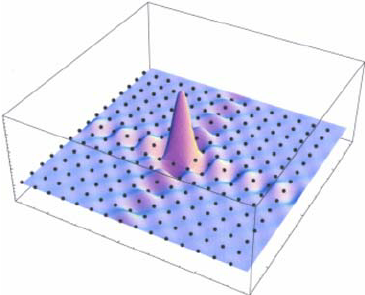
\includegraphics[width=0.5\textwidth]{psinc}
%\caption{An illustration of the periodic cardinal sin function (psinc) basis set used to expand the NGWFs in ONETEP.\cite{psinc}}
%\end{figure}
%
To achieve linear-scaling, it is not efficient to work in terms of the aforementioned electron density ($n(\mathbf{r})$) from the Kohn-Sham equations, and instead formulate the problem in terms of a density matrix defined by (Eq.~\ref{densitymatrix}), where ($f_n$) is the occupancy and ($\psi$) the KS orbitals. It has the property of idempotency ($\rho^2 = \rho$), the electron density can be computed as its diagonal elements ($n(\mathbf{r}) = 2 \rho(\mathbf{r, r'})$) and the total energy of a system is defined as ($E = 2\mathrm{Tr} (\rho H)$).
%
\begin{equation} \label{densitymatrix}
\rho(\mathbf{r, r'}) = \sum_n f_n \psi_n(\mathbf{r}) \psi_n^*(\mathbf{r'})
\end{equation} 
%
Specifically within ONETEP, the density matrix is given in terms of non-orthogonal generalised Wannier functions (NGWFs) that are localised in real space,\cite{psinc} and defined by (Eq.~\ref{ngwf}). The density kernel ($K^{\alpha \beta}$) is a representation of ($f_n$) (Eq.~\ref{densitymatrix}) and must be sparse, so that elements of the NGWF further than a defined cut-off ($r_K$) can be truncated.
%
\begin{equation} \label{ngwf}
\rho(\mathbf{r, r'}) = \sum_{\alpha \beta} \phi_{\alpha} (\mathbf{r}) K^{\alpha \beta} \phi_{\beta}^*(\mathbf{r})
\end{equation}
%
The ground state energy of a given system is then computed by (Eq.~\ref{onetepmin})
%
\begin{equation} \label{onetepmin}
E_0 = \min_n E[n] = \min_\rho E[\rho]_{\rho = \rho^2} = \min_{\mathbf{K}, \phi} E[\mathbf{K}, \phi]
\end{equation}
%
By (Eq.~\ref{onetepmin}), two nested conjugate gradient constrained search loops are used to minimise the total energy. In the outer energy minimisation loop, the density kernel is kept fixed while the energy is minimised with respect to the spatial profile of the NGWFs, which is equivalent to solving a KS eigenvalue problem. In the inner loop, the NGWF expansion is kept fixed while the energy is minimised with respect to the matrix elements of the density kernel. Therefore eventually arriving at a self-consistent Hamiltonian once the right (idempotent) density matrix ($\rho(\mathbf{r, r'})$) is found. %An illustration of an extended eigenstate compared with a localised NGWF is given in figure \ref{fig:oligo}.
%
%\begin{figure}[H]
%\centering
%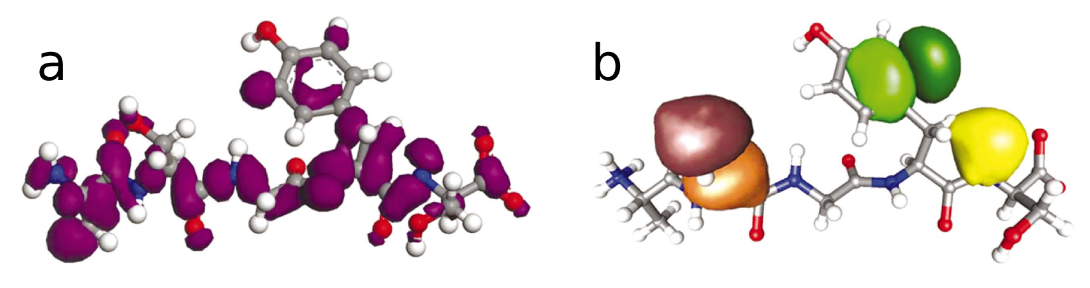
\includegraphics[width=0.99\columnwidth]{ngwf}
%\caption{(a) An extended eigenstate for an oligopeptide molecule, (b) localised NGWFs for the same molecule.\cite{psinc}}
%\label{fig:oligo}
%\end{figure}
%
\subsection{Bespoke non-bonded forcefield parameters}\label{sec:ddec}
%
The Tkatchenko-Scheffler (TS) method is an approach to post process the ground state electronic density --- produced by the DFT calculations as outlined in (section \ref{sec:linear_scaling}) --- to derive the non-bonded forcefield parameters from (Eq.~\ref{eq:forcefield}) for use in MD simulations.\cite{tkatchenko2009accurate} It utilises the charge density dependence of both atomic charges as well as Lennard-Jones parameters, therefore accounting for the impact of the local chemical environment on the van der Waals contributions and point charges of atoms. The TS \edit{method} requires an atoms-in-molecule method, which uses the ground state DFT electronic density of the molecular system ($n(\mathbf{r})$) to divide into uniform overlapping atomic densities ($n_{A}(\mathbf{r})$) through a weighting factor $w_{A}(\mathbf{r})$ (Eq.~\ref{eq:TS}).\cite{tkatchenko2009accurate,manz2012improved}
%
\begin{equation} \label{eq:TS}
n_{A}(\mathbf{r})=w_{A}(\mathbf{r})\,n_{\mathrm{mol}}(\mathbf{r})
\end{equation}
%
The weighting factor is calculated by computing the share of each isolated atom ($n_{A}^0(\mathbf{r})$) of the ($N$) atoms that make up a promolecule ($n_{\mathrm{mol}}^0(\mathbf{r})$). A promolecule is an ideal reference system composed of non-interacting atoms fixed at the same positions in the corresponding molecular system.
\begin{equation}
    n_{\mathrm{mol}}^0(\mathbf{r}) = \sum_{A=1}^N n_{A}^0(\mathbf{r})
\end{equation}
where the weighting factors are differently formulated according to the atoms-in-molecule scheme, in the iterative Hirshfeld (IH) scheme,\cite{bultinck2007uniqueness} it is given by:
\begin{equation}
    w_{A}^{\mathrm{IH}}(\mathbf{r}) = \frac{n_{A}^0(\mathbf{r})}{n_{\mathrm{mol}}^0(\mathbf{r})}
\end{equation}
The self-consistency of the IH scheme therefore requires that the share of the isolated atomic densities ($n_{A}^0(\mathbf{r})$) from the promolecular density ($n_{\mathrm{mol}}^0(\mathbf{r})$) is equivalent to the share of the overlapping atomic density ($n_{A}(\mathbf{r})$) from the total molecular density ($n_{\mathrm{mol}}(\mathbf{r})$). The atomic electron population ($N_A$) are derived from the atomic densities ($n_{A}(\mathbf{r})$) by:
%
\begin{equation}
    N_A = \int n_A (\mathbf{r}) \mathrm{d}\mathbf{r}
\end{equation}
%
In the IH scheme, the isolated atomic density is composed of the weighted average of the atomic densities with the next lowest integer ($\mathrm{lint}(N_A)$) and next highest integer ($\mathrm{uint}(N_A)$) occupancies. %
\begin{equation}
\begin{aligned}
n_{A}^{0, N_{A}}(\mathbf{r})=& \,\,n_{A}^{0, \operatorname{lint}\left(N_{A}\right)}(\mathbf{r})\left[\operatorname{uint}\left(N_{A}\right)-N_{A}\right] \\
&+n_{A}^{0, \operatorname{uint}\left(N_{A}\right)}(\mathbf{r})\left[N_{A}-\operatorname{lint}\left(N_{A}\right)\right]
\end{aligned}
\end{equation}
The weighting factor in the iterated stockholder atoms (ISA) scheme \cite{lillestolen2008redefining} is instead defined with respect to the spherical average of the electronic density around atom ($A$) by (Eq.~\ref{eq:ISA_weights}). Unlike IH, the self-consistency in ISA requires that every value of the radius of a sphere around each nucleus ($A$), the average electron density on the surface of this sphere is the same in the promolecular atom ($\langle n_{A}^{0, \mathrm{ISA}}(d)\rangle$) and in the atom in the molecule ($\langle n_{A}^{\mathrm{ISA}}(d)\rangle$).\cite{bultinck2009comparison}
%
\begin{equation} \label{eq:ISA_weights}
w_{A}^{\mathrm{ISA}}(\mathbf{r})=\frac{\left\langle n_{A}^{0,\mathrm{ISA}}\left(\left|\mathbf{r}-\mathbf{R}_{A}\right|\right)\right\rangle}{n_{\mathrm{mol}}^{0, \mathrm{ISA}}(\mathbf{r})}
\end{equation}
where ($\langle n_{A}^{0, \mathrm{ISA}}\left(\left|\mathbf{r}-\mathbf{R}_{A}\right|\right)\rangle$) is the average density over the surface of a sphere with radius ($d$) for an isolated atom ($A$). The promolecular density in (Eq.~\ref{eq:ISA_weights}) is similarly defined as the sum of spherically averaged spheres of radii ($|\mathbf{r} - \mathbf{R}_B|$) around every atom ($B$):
%
\begin{equation}
n_{\mathrm{mol}}^{0, \mathrm{ISA}}(\mathbf{r})=\sum_{B=1}^{N}\left\langle n_{B}^{0, \mathrm{ISA}}\left(\left|\mathbf{r}-\mathbf{R}_{B}\right|\right)\right\rangle
\end{equation}
The density derived electrostatic and chemical electron density partitioning (DDEC) method is one of the atoms-in-molecule electronic density partitioning approaches. DDEC uses a mixture of both IH and ISA methods and iteratively optimises for a converged solution to the weighing factor to resemble the spherical average of the atomic densities ($n_{A}(\mathbf{r})$) and the density of an isolated reference atom ($n_{A}^0(\mathbf{r})$). The atomic partial charges ($q_A$) for MD are derived from DDEC by (Eq.~\ref{eq:ddec_charge}), where ($Z_A$) is the nuclear charge of atom $A$. 
%
\begin{equation} \label{eq:ddec_charge}
    q_A = Z_A - N_A = Z_A - \int n_A(\mathbf{r}) \, \mathrm{d}^3 \mathbf{r}
\end{equation}
%
Whereas the dispersion ($B_{ij}$) and repulsion ($A_{ij}$) coefficients are derived from the partitioned electronic density by (Eq.~\ref{eq:qube_bij}) and (Eq.~\ref{eq:qube_aij}).\cite{horton2019qubekit}
\vspace{-2mm}
\begin{subequations} 
\begin{align}
\begin{split}\label{eq:qube_bij}
B_{i}=\left(\frac{V_{A}^{\mathrm{DDEC}}}{V_{A}^{\mathrm{free}}}\right)^{2} B_{i}^{\mathrm{free}}
\end{split}\\
\begin{split}\label{eq:qube_aij}
A_{i}=\frac{1}{2} B_{i}\left(2 R_{A}^{\mathrm{DDEC}}\right)^{6}
\end{split}
\end{align}
\end{subequations}
%
The atomic volume ($V_{A}^{\mathrm{DDEC}}$) is calculated from the electronic density:
%
\begin{equation} \label{eq:qube_volume}
V_{A}^{\mathrm{DDEC}}=\int r^{3} n_{A}(\mathbf{r}) \, \mathrm{d}^{3} \mathbf{r}
\end{equation}
%
Whereas the other terms are derived from alternative methods. Namely, the free dispersion coefficients ($B_{i}^{\mathrm{free}}$) are computed using time-dependent DFT calculations of free atoms in vacuum,\cite{chu2004linear} the reference volume ($V_{A}^{\mathrm{free}}$) is calculated using more accurate \textit{ab initio} approaches with explicit treatment of electron correlation effects and the DDEC effective radius of each atom rescales the experimentally derived reference free atom radius ($R_{A}^{\mathrm{free}}$) using (Eq.~\ref{eq:qube_radius}).\cite{horton2019qubekit} 
%
\begin{equation} \label{eq:qube_radius}
R_{A}^{\mathrm{DDEC}}=\left(\frac{V_{A}^{\mathrm{AIM}}}{V_{A}^{\mathrm{free}}}\right)^{1 / 3} R_{A}^{\mathrm{free}}
\end{equation}
%
The dispersion and repulsion coefficients are related to the Lennard-Jones parameters, ($\epsilon$) and ($\sigma$), (Eq.~\ref{eq:forcefield}) via ($A_{ij} = 4 \epsilon_{ij}\,\sigma_{ij}^{12}$) and ($B_{ij} = 4 \epsilon_{ij}\,\sigma_{ij}^{6}$). The resulting parameters are an accurate representation of the chemistry of the molecular system under investigation, since they are exclusively derived from \textit{ab initio} quantum mechanical calculations. As such, computing the non-bonded forcefield parameters using DDEC is a basis for bespoke forcefield parametrisation to bypass the use for transferable forcefields. This approach is implemented for small molecules by software such as QUBEKit.\cite{horton2019qubekit} 

%\newpage
\section{\edit{Dynamical Mean Field Theory}}
%
\edit{Strongly correlated materials --- encompassing many transition metal oxides --- typically have incompletely-filled $d$- or $f$-shells, where the on-site Coulombic interactions are comparable with the band-gap. Electronic correlations in such systems give rise to complex behaviour that can no longer be described by the treatment of a single electron within a system of non-interacting particles. As such, single-electron theories such as the local-density approximation (LDA) in density functional theory (DFT) or Hartree-Fock theory fail to accurately describe their electronic structure.\cite{anisimov2010electronic}}

\edit{Strongly correlated materials embody exotic electronic properties that are technologically advantageous or have evolved to be utilised by nature for biological function.\cite{al2020superexchange, weber13, Weber2014a} A study of the Hemocyanin protein core in Chapter requires such a treatment, where extensions to DFT methods are necessary to accurately describe the electronic structure of the strongly correlated metalloprotein active site.\cite{al2020superexchange}}
%
\subsection{\edit{Hubbard model}}
%
\edit{The Hubbard model is a lattice model that describes the interaction of particles of opposite spin on a lattice with sites ($i,j$) through on-site electronic repulsion ($U$) and off-site kinetic hopping ($t$) terms.\cite{kanamori1963electron, hubbard1963electron, gutzwiller1963effect} The Hubbard model Hamiltonian (Eq.~\ref{eq:hubbard_model}) is defined with respect to the creation ($c^{\dagger}$) and annihilation ($c$) operators, for spin indices ($\sigma$) and the occupation of the $i$-th site ($n_i$), where $n_{i \sigma} = c_{i \sigma}^{\dagger} c_{j \sigma}$}.\cite{Anisimov1991a}
%
\begin{equation} \label{eq:hubbard_model}
    \hat{H}_{\mathrm{Hubbard}}=t \sum_{\langle i j\rangle \sigma} c_{i \sigma}^{\dagger} c_{j \sigma}+U \sum_{i} n_{i \uparrow} n_{i \downarrow}
\end{equation}

\edit{Despite its simplistic formulation, the Hubbard model --- unlike conventional approaches --- correctly describes the insulating character of Mott insulators by accounting for the strong repulsion between electrons. In the limit of infinite dimensions or lattice coordination number, the Hubbard model is an exact treatment of the local correlations of a strongly correlated system.\cite{metzner1989correlated}}

\subsection{\edit{Anderson impurity model}}

\edit{The Anderson impurity model (AIM) is a model Hamiltonian that describes magnetic impurities embedded in a metallic system. It is formulated with respect to the intra-site Coulomb repulsion of the impurity energy levels ($\hat{H}_{\mathrm{loc}}$), a bath of conducting electrons ($\hat{H}_{\mathrm{bath}}$) and the coupling term between the impurity and conduction orbitals ($\hat{H}_{\mathrm{mix}}$).\cite{anderson1961localized}}

\begin{equation} \label{eq:AIM}
{H}_{\mathrm{AIM}}=\overbrace{\sum_{i} \epsilon_{i} a_{i}^{\dagger} a_{i}}^{\hat{H}_{\text {bath}}}+\overbrace{\sum_{i \sigma}\left(V_{i}^{\sigma} c_{\sigma}^{\dagger} a_{i \sigma}+ \mathrm{h . c.} \right)}^{\hat{H}_{\text {mix}}}+\overbrace{U n_{\uparrow} n_{\downarrow}-\mu\left(n_{\uparrow}+n_{\downarrow}\right)}^{\hat{H}_{\mathrm{loc}}}
\end{equation}

\edit{The non-correlated electronic levels ($\epsilon_{i}$) of the bath are defined with respect to bath creation ($a_{i}^{\dagger}$) and annihilation ($a_{i}$) operators. The impurity is described by electrons ($n$) interacting through a Coulomb repulsion ($U$) and a chemical potential ($\mu$). The coupling between the impurity and bath orbitals is described by the hybridisation term ($V_{i}^{\sigma}$).}

\edit{The dynamics of the electrons hopping into and out of the bath are described by the impurity Green's function ($G_{\text{imp}}$) and defined with respect to the hybridisation function ($\Delta (\omega) =\sum_{k}\left|V_{k}\right|^{2} /\left(\omega+\mu-\epsilon_{k}\right) $) and the self energy ($\Sigma (\omega)$) for frequency ($\omega$):}
%
\begin{equation}
    G_{\text {imp }}\left(\omega\right) ^ {-1} = \omega+\mu-\epsilon_{k}- \Delta (\omega) - \Sigma_{imp}\left(\omega\right)
\end{equation}
%
\edit{In dynamical mean-field theory (DMFT),\cite{Georges1996a} the lattice (Hubbard) model can be mapped onto a single impurity model, where the single correlated impurity orbital is embedded in an uncorrelated bath of conduction-band states. This mapping is self-consistent, requiring the impurity Green's function to reproduce the lattice dynamics, as described by the local lattice Green's function ($G_{\text{ii}}$), such that:}
%
\begin{equation}
    G_{\text {imp }}\left(\omega\right) = G_{\text {ii}}\left(\omega\right)
\end{equation}
%
\edit{As well as the self-energy:}
%
\begin{equation}
    \Sigma_{\text {imp }}\left(\omega\right) = \Sigma_{\text {ii}}\left(\omega\right)
\end{equation}
%
\edit{A DMFT calculation is solved through an iterative process where the AIM parameters are chosen such that the model Hamiltonian best describes the physics of the real system in question. As the hybridisation function encapsulates all of the contributions of the bath sites to the physics of the impurity sites, the iterative process converges when the hybridisation function satisfies the self-consistency conditions outlined above.\cite{linscott2020onetep}}

\edit{DMFT is a sophisticated method that includes quantum dynamical effects, and takes into account charge fluctuations, spin fluctuations, and thermal excitations. The DMFT approach is very computationally expensive for studying realistic systems, it is therefore combined with DFT in the form of DFT+DMFT to result in a method that belongs to a broad category of embedding approaches.\cite{Georges1996a,dca_reference_cluster_dmft} The DFT+DMFT method accounts for the limitations of DFT by treating the many-body effects of strongly correlated materials explicitly, while limiting this treatment to the correlated subspace of the $d$- or $f$-electrons, thereby side-stepping the prohibitive scaling of quantum chemistry methods.}
\chapter{Interpretation of morphogen gradients by a synthetic bistable circuit}
\label{chapter:double-exclusive}
%\epigraph{``No person will deny that the highest degree of attainable accuracy is an object to be desired, and it is generally found that the last advances towards precision require a greater devotion of time, labour, and expense, than those which precede them."}{Charles Babbage}
\vspace{-9mm}
Contributions for this work are as follows: \textbf{Mohamed Ali al-Badri} and \textbf{Christian D. Lorenz} conceived and planned the research. \textbf{Mohamed Ali al-Badri} and \textbf{Robert C. Sinclair} developed the nanomaterial structure software. \textbf{Mohamed Ali al-Badri} performed the calculations. \textbf{Mohamed Ali al-Badri, Paul Smith} and \textbf{Christian D. Lorenz} analysed the data and \textbf{Mohamed Ali al-Badri} prepared the final manuscript.

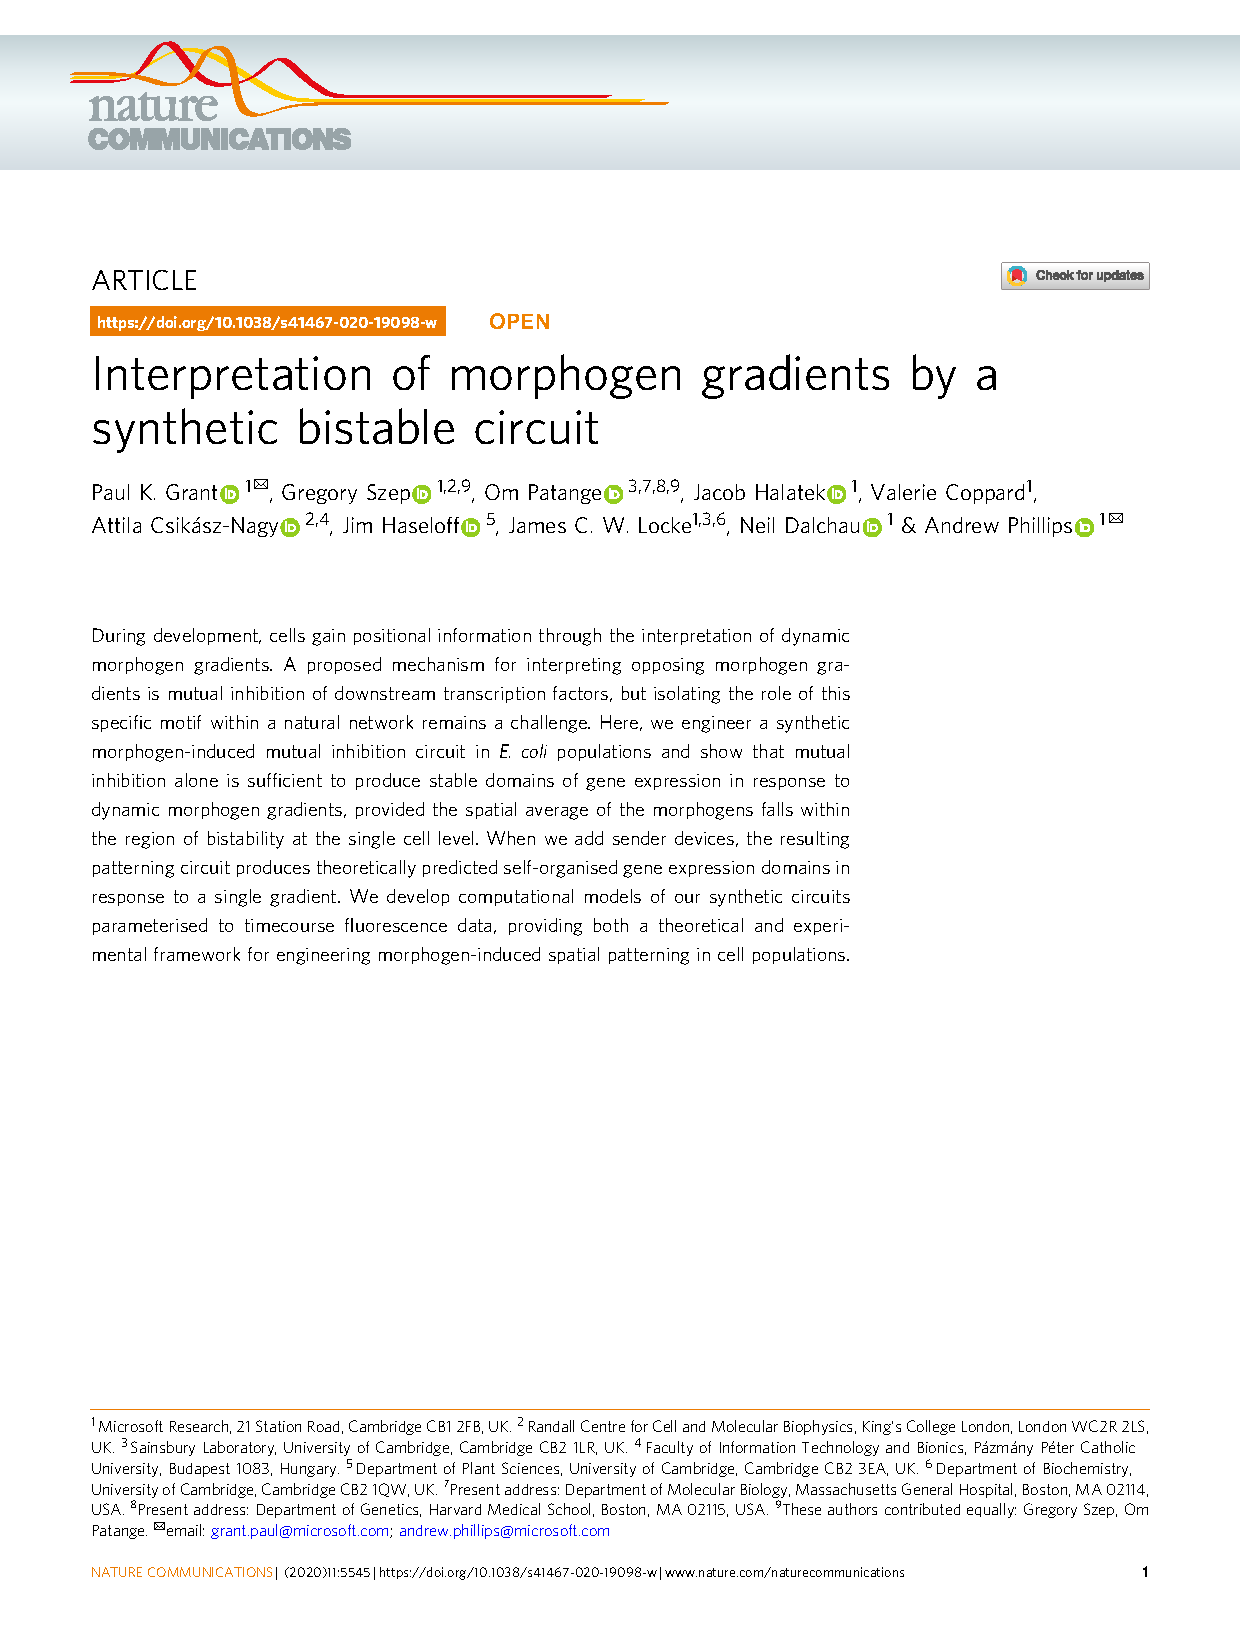
\includepdf[pages=-, offset=75 -75, addtotoc={
        2,section,1,Introduction,section:introduction,
        2,section,1,Results,section:results,
        2,subsection,2,Engineering mutual exclusivity,exclusivity,
        3,subsection,2,Mutual inhibition results in bistability,bistability,
        4,subsection,2,Hysteresis produces stable boundaries,boundaries,
        4,subsection,2,A secondary gradient creates self-organised domains,self-organisation,
        5,section,1,Discussion,section:discussion,
        6,section,1,Methods,section:methods,
        6,subsection,2,Plasmid construction,plasmids,
        6,subsection,2,Plate fluorometer assay,plates,
        6,subsection,2,Flow-cytometric analysis of hysteresis,flow,
        7,subsection,2,Microfluidics,microfluidics,
        7,subsection,2,Microfluidics microscopy,microscopy,
        7,subsection,2,Solid culture assays,cultures},
    addtolist={
        2, figure, {\textbf{A synthetic gene circuit for morphogen interpretation}. \textbf{a} Schematic representation of a developing embryo. Mutual inhibition of transcriptionfactors (cyan and yellow) downstream of antiparallel morphogen gradients (dark blue and orange) has been hypothesized to produce mutually exclusive domains of gene expression. \textbf{b} Morphogen gradients can be dynamic and transient, yet sharp, stable boundaries are observed between domains of gene expression. \textbf{c} A diagram of the Exclusive Receiver circuit. When 3O-C12-HSL (C12) levels are high, C12 binds to LasR, activating the expression of YFP and TetR, which represses the expression of LuxR, preventing expression of CFP and LacI. When 3O-C6-HSL (C6) levels are high, C6 binds to LuxR activating expression of CFP and LacI, which represses the expression of LasR, preventing expression of YFP and TetR. \textbf{d} Fluorescence output, measured in microplate fluorometer assays, of the Exclusive Receiver (top) and the Receiver (bottom) circuits represented as a ratio of CFP- (left) or YFP- (right) fluorescence to RFP fluorescence during exponential phase, cultured in the presence of the concentrations of C6 and C12 indicated. Data are representative of $n=3$ biological replicate experiments conducted on different days}, figure:overview,
        3, figure, {\textbf{Mutual inhibition produces bistability}. Cells transformed with the Exclusive Receiver circuit were conditioned in either 500 nM C6 \textbf{a}, or 500 nM C12 \textbf{b}, and then exposed to the combinations of concentrations of C6 and C12 indicated.  Cells were measured using flow cytometry and their normalized CFP minus YFP expressions were plotted. The region of bistability predicted by the parameterized model is the area within the red lines.  \textbf{c}, Microfluidics cultures of cells transformed with Exclusive Receiver circuit in changing combinations of signals.  Cells were grown for 3 hours in the presence of either 37 nM C6 (rows 1 and 2) or 100 nM C12 (rows 3 and 4). Then media was changed to 100 nM C12 + 37 nM C6 (rows 1 and 3) or 100 nM C12 (row 2) or 37 nM C6 (row 4) . Cells were imaged with a frame rate of (1 frame/10 minutes). Left panels are kymographs of the log-ratio of CFP expression per-cell to YFP expression per-cell, and fraction of cells as a heat map.  Histograms represent the populations at 3 hours (red) and 8 hours (blue).  Lines and shaded region represent the mean and standard deviation, respectively, over {n = 4  biological replicates performed on 4 different days.} Right panels are sample montages of cells switching state (rows 2 and 4) or exhibiting bistablity (rows 1 and 3); phase contrast and fluorescence channel ranges chosen for display. Scalebar=6$\mu$m.}, figure:bistability,
        5, figure, {\textbf{Formation of stable boundaries.} \textbf{a}, Endpoint fluorescence microscopy of Exclusive Receiver cells grown in transient gradients of signals (C12 diffusing from the left, C6 diffusing from the right) at the spatial average concentrations indicated and in the context of 10 $\mu$M IPTG throughout.  Representative examples (n=3 biological replicates performed on 3 different days) of a static boundary (left) and a moving boundary (right) \textbf{b}, Corresponding kymographs of CFP and YFP fluorescence (intensity) over time (y-axes, hours) at different spatial positions (x-axes, mm). If the location of the boundary (location of equal normalized CFP and YFP fluorescences, black lines) at the end of the timelapse minus its location when it became detectable ($\Delta\beta$, arrows) was less than 10\% of the domain size we considered the boundary stable.   \textbf{c}, Boundaries were evaluated as above at the signal concentrations indicated by letters. ‘S’ indicates equilibrium concentrations at which static boundaries were observed. ‘M’ indicates a moving boundary. 'N' indicates no boundary.  The color of the letter indicates which FP was dominant and red indicates neither FP dominant. \textbf{d}, Schematic representation of the concentrations of C6 and C12 experienced by cells at different points in physical space (cyan and yellow curves) as gradients diffuse to homogeneity.  Paler curves represent different timepoints.  If the spatial average concentrations lie within the region of bistability, the boundary will be static (S), otherwise the boundary will move (M) and will eventually be abolished as cells adopt either CFP or YFP expression.   $t_1$ and $t_2$ indicate timepoints considered in (e).  \textbf{e}, Corresponding schematic representing LasR expression, colored according to resultant fluorescent protein expression.  Dashed line indicates the location of an unstable local equilibrium. Red lines indicate the spatial location in which cells are exhibiting bistability.  In the case of a stationary boundary (S), the region of space containing cells exhibiting bistability expands to encompass all cells and their gene expression state is determined by their history.  In the case of a moving boundary (M), the region exhibiting bistability moves rightward and disappears and the domain becomes dominated by a single monostable state.}, figure:boundaries,
        6, figure, {\textbf{Addition of a Relay circuit creates self-organised domains of gene expression.} \textbf{a}, Circuit diagram of Exclusive Receiver cells co-transformed with a  Relay circuit  (P76-LasI) that responds to C6 by producing C12. \textbf{b}, Isogenic cells transformed with the circuit shown in (a) and grown for 24 hours in the presence of a gradient of C6 diffusing from the centre. Cells that experience high levels of C6 (central cells) will express CFP, LacI, and LasI, causing them to produce C12 but be unable to sense it.  Neighbouring cells (outer cells) that do not experience C6 will sense C12 and express YFP and TetR, resulting in mutually exclusive domains of gene expression.{ Cells also constitutively express mRFP1 via a genomic transgene. Image is representative of 3 biological replicates performed on 3 different days.} \textbf{c}, Quantitation of fluorescence along the dotted line in b. Cyan, yellow, and red indicate CFP, YFP, and RFP expression, respectively. \textbf{d}, Final timepoint of simulation shows a secondary gradient of C12 (orange) produced in response to the primary C6 gradient (dark blue).  Cyan and yellow indicate simulated CFP and YFP expression, respectively.  \textbf{e}, Final time point of simulation in C6-C12 space labelling points in physical space by their CFP and YFP expression (cyan and yellow points), and showing the production of C12 as vectors (red arrows) that move the spatial average (x) toward increasing C12}, figure:relay
}]{publications/double-exclusive.pdf}
% \chapter{Parameter Inference with Bifurcation Diagrams}
\label{chapter:inference}

%\epigraph{\textit{I Have divers times endeavoured to see and to know, what parts the Blood consists of; and at length I have observ’d, taking some Blood out of my own hand, that it consists of small round globuls driven thorough a Crystalline humidity or water: Yet, whether all Blood be such, I doubt.}}{Antoni Van Leeuwenhoek}

%\begin{center}
%    \textit{The contents of this chapter are under review with Nanoscale Horizons}
%\end{center}

The work in this chapter extends on the accurate modelling of graphene oxide nanomaterials to investigate changes in protein structure upon adsorption on the material. Using molecular dynamics simulations, we study the evolution of protein structure in response to interfacial interactions on the bio-nano interface. To understand the impact of structural changes over simulation times of hundreds of nanoseconds, we require a comprehensive analysis pipeline that investigates these changes from multiple perspectives. Here, we probe the varying adsorption behaviours of apolipoprotein c-III and the effect of functional groups in modulating protein aggregation on the nanomaterial. We use two functionalisations of graphitic materials --- graphene oxide and double-clickable graphene oxide.

\edit{Contributions for this work are as follows: \textbf{Mohamed Ali al-Badri} and \textbf{Christian D. Lorenz} conceived and planned the research. \textbf{Mohamed Ali al-Badri} performed the calculations. \textbf{Mohamed Ali al-Badri, Paul Smith} and \textbf{Christian D. Lorenz} analysed the data and \textbf{Mohamed Ali al-Badri} prepared the final manuscript.}
%Contributions for this work are as follows: \textbf{Mohamed Ali al-Badri}: Conceptualisation, Methodology, Software, Validation, Formal analysis, Investigation, Writing - original draft, Visualisation. \textbf{Paul Smith}: Methodology, Software \edit{development for analysis scripts}, Validation, Formal analysis, Visualisation.
\clearpage

The protein corona is an obstacle to exploiting the exotic properties of nanomaterials in clinical and biotechnology settings, with potential applications in DNA sequencing, point of care testing and drug delivery vehicles. The formation of the protein corona is driven by dynamic atomic scale interactions at the bio-nano interface, which are impenetrable using conventional experimental techniques. Here, we use molecular dynamics simulations to study the effect of graphene-oxide (GO) functionalisation on apolipoprotein-c3 (apo-c3) adsorption. We develop an analysis pipeline, encompassing binding energy calculations to protein structure analyses employing \edit{Uniform Manifold Approximation and Projection for Dimension Reduction (UMAP)} and machine learning clustering. We find that apo-c3 is denatured by adsorption on GO, largely driven by the large energetic contributions of electrostatic interactions such as $\pi$-$\pi$ stacking of aromatic amino acids to pristine graphene regions. The enthalpic contribution of such binding event outweighs the intraprotein bond enthalpy required to maintain the protein tertiary structure. Through denaturing and exposing buried hydrophobic residues, the protein backbone is stabilised by forming $\beta$-bridges, which serve as binding motifs for protein-protein interactions that drive further protein aggregation on the nanomaterial surface. When adsorbing on double-clickable azide- and alkyne-double functionalised graphene oxide (C2GO), apo-c3 largely retains its tertiary structure. Binding with the nanomaterial surface is dominated by weaker van der Waals interactions that are dispersed over the protein surface, where charged protein residues are sterically hindered by azide functional groups. The apo-c3 N-terminus is the binding motif for C2GO adsorption, leaving the  conformation of the C-terminus unchanged, hence conserving the lipid binding function of apo-c3.

\section{Introduction}

Graphene-oxide (GO) is a semi-ordered 2D material that shares many novel mechanical and electronic properties with graphene. It is utilised in applications including ion trapping, desalination, electronics, chemistry and biomedicine.\cite{yuan2017enhanced, zhu2010graphene, chung2013biomedical} GO is a promising platform for \textit{ex} and \textit{in vivo} biological applications --- such as bio-sensing and therapeutics. Its electrochemical properties makes GO an attractive contender for bio-sensing applications such as single nucleotide polymorphism detection in DNA,\cite{bonanni2012inherently} next generation nanopore DNA sequencing \cite{heerema2016graphene} and point of care (PoC) applications for early virus detection using covalently linked immobilised monoclonal antibodies.\cite{afsahi2018novel} Therapeutically, the large surface area to volume ratio of 2D materials results in a large loading capacity for targeting molecules, fluorescent dyes and drug molecules for intravenous administration as well as photothermal therapy for cancer treatment.\cite{robinson2011ultrasmall, liu2013graphene, sun2008nano, zhang2010functional}  \\

Unfortunately the transition from \textit{in vitro} to clinical settings is held back by a chemically driven adsorption of serum proteins --- referred to as a protein corona --- upon their introduction to a biological medium.\cite{casals2010time, ke2017decade} A hard corona (HC) is a tightly bound monolayer of proteins at the nanoparticle interface. Subsequent protein layers adherent to the HC are referred to as the soft corona (SC).\cite{rocker2009quantitative} The character and composition of the HC define the nanomaterial's biological identity and therefore its biological fate, circulation time, cellular uptake and cytotoxicity.\cite{nierenberg2018formation, mei2018protein} HC formation has revealed highly variant protein composition profiles, sensitive not only to inter-species biological media \cite{solorio2017comparison} but also disease-specific influences in human GO coronas.\cite{hajipour2015personalized} Patient-specific or `personalised' protein corona profiles have since been utilised as a diagnostic tool for high-throughput, inexpensive and highly accurate early cancer detection.\cite{papi2019converting} \\

Modulating the HC character to overcome the disadvantages of 2D materials in biological applications through nano-functionalisation remains challenging.\cite{rampado2020recent} Extrapolating the sensitivity of nano-functionalisation to the aforementioned highly variant identity of the corona from experimental studies is incomplete and requires a better understanding of GO-HC interfacial behaviour to atomistic precision. Such an understanding is paramount to designing the next generation of biosensors and nanomedicines.\\

Azide- and alkyne-double functionalised graphene oxide (C2GO) has previously been proposed as a cancer targeting nanovector,\cite{mei2015synthesis} where click reactions conjugate targeting moieties on azide and trimethylsilyl (TMS)-alkyne functional groups.\cite{rubio2015solvent} In vitro, both C2GO and GO show varying HC character when exposed to serum proteins, which subsequently impacts their biological identities.\cite{mei2018protein} An experimental quality-by-design screening platform was used to unpick the HC character and evaluate its relationship with biological fate, cellular uptake and cytotoxicity. Using this, proteins that reduced material dependent toxicities were identified to play a role in diminishing cytotoxicity, including apolipoprotein C-III (apo-c3).\cite{mei2018protein} \\

Protein coronas are known to temporally evolve, leaving the total amount of protein constant but varying their composition according to binding affinity, known as the Vroman effect.\cite{vroman1980interaction} Upon the introduction of a nanomaterial to a biological medium, highly abundant proteins such as albumin, immunoglobulin G and fibrinogen bind to the nanoparticle surface in the early stages of the Vroman effect, followed by their replacement with high binding affinity proteins such as apolipoproteins and coagulation factors in the late stages of the Vroman effect.\cite{foroozandeh2015merging, ehrenberg2009influence, harnisch2000adsorption, goppert2005polysorbate, vroman1980interaction} The Vroman effect has previously been observed in computational and experimental studies of peptide, cellulose and fatty-acid binding on GO.\cite{radic2013competitive} \\

 Previously, MD has been used to study the interactions of GO with peptides to understand conformational transitions of amyloid-beta during adsorption,\cite{baweja_effect_2015} the hydration pattern of an adsorbed toy-model alpha-helix \cite{baweja2013hydration} and verification of enzyme active-site deformation following adsorption. \cite{sun_mechanism_2014} To the best of our knowledge, no MD simulations have so far studied protein adsorption on accurate models of GO, and have instead randomly placed oxidised functional groups on the GO surface. Accurate modelling of GO should reflect the semi-ordered structure of GO; composed of inhomogeneous regions of oxidised and unoxidised domains, where amorphous alcohol and epoxy groups make up the oxidised regions.\cite{sinclair2019modelling} \textit{Ab initio} MD simulations of GO show that semi-ordered models of GO are the most stable structures in vacuum as well as in liquid water.\cite{mouhat2020structure} Furthermore, we have recently shown the importance of accurate functionalisation and accounting for steric strain and edge functional groups in large scale MD simulations of GO, using generalised and bespoke electronic structure MD forcefield design.\cite{al2020accurate} In this work, we use molecular dynamics (MD) simulations to study protein denaturing through adsorption on GO and C2GO, to understand HC conformation-activity relationships through binding free energy, contact map, protein structure and solvent exposure analyses. We apply machine learning dimensionality reduction techniques to decode the spatio-temporal MD data that is hard to interpret into distinct protein secondary structure conformations.
%--------------------------------------
%
%               RESULTS
%
%--------------------------------------
\section{Results}
%
\subsection{Binding on the bio-nano interface}
%
In both GO and C2GO systems, apo-c3 readily adsorbs to the substrate and reaches a stable conformation over the course of the adsorption trajectory. To investigate the binding of apo-c3 to the GO and C2GO interface, we compute contact maps and free energies of binding that underpin the changes in protein structure following adsorption. These analyses probe interfacial dynamics that may play a large role in the formation of a protein corona around a nanomaterial upon its introduction to a biological medium. To identify adsorption of apo-c3 to the graphitic sheets we calculated the minimum distance over time between any heavy (non-hydrogen) atom of the protein to any heavy atom of the sheet (Fig.~\ref{fig:mid-dist-to-grap}). We also compute the minimum distance of each residue to the graphitic sheets over time. These are combined to produce a heatmap of contact probability between apo-c3 and GO/C2GO (Fig.~\ref{fig:contacts}B). The binding free energy is calculated according to the molecular mechanics with Poisson–Boltzmann and surface area solvation (MM-PBSA) method, implemented using g\_mmpbsa.\cite{kumari2014g_mmpbsa}\\

\begin{figure*}
    \centering
    \includegraphics[width=\textwidth]{figures/contacts-energies-fixed.png}
    \caption{MM-PBSA binding energy contributions per apo-c3 amino acid residue for GO and C2GO sheets, colour coded by magnitude (A), heat map showing contact probability of apo-c3 amino acid type with GO and C2GO functional group atoms (B) and adsorbed apo-c3 structure on GO and C2GO, protein amino acids at the graphitic interface are coloured by MM-PBSA binding energy contribution and hydrogen atoms have been omitted for clarity (C).}
    \label{fig:contacts}
\end{figure*}
%
The average binding free energy components for the GO-apo-c3 and C2GO-apo-c3 systems are given in Table 1. The binding free energy components are decomposed to per-residue contributions (Fig.~\ref{fig:contacts}A). In this way we can acquire a better understanding of each amino-acid's contribution to the binding free energy of the protein-nanomaterial complex. Per-residue binding free energy contributions are colour-coded by their interaction strength (blue to red) in the protein structure of the final configuration (Fig.~\ref{fig:contacts}C) for GO and C2GO, where each largely contributing amino acid residue has been illustrated and labelled explicitly. \edit{Note that the entropic contribution to the binding free energy is not calculated using high-throughput methods such as g\_mmpbsa, due to their computational cost. Therefore, the binding free energies in (Table 1) are computed to evaluate the relative binding free energy instead of the absolute free energy.}\\

The binding of apo-c3 to the graphitic substrate is driven by amino acids with the highest binding affinities from the beginning of the adsorption process. Apo-c3 residues 60-70 initiate binding with GO (Fig.~\ref{fig:mid-dist-to-grap}), most likely due to the high binding affinity of TRP65 to $\pi$-$\pi$ stack with pristine graphene domains on the GO surface, as well as GLU63 binding with positively charged (tertiary alkyl, phenol and carboxylic acid) carbon atoms (Fig.\ref{fig:contacts}A). From 100 ns apo-c3 binding to GO is driven by positively charged (HIS18, LYS21) and polar (THR20) residues (Fig.\ref{fig:contacts}A) interacting with oxygen containing surface functional groups. Accordingly, the binding free energy of GO-apo-c3 has a higher net contribution of electrostatic interactions when compared with C2GO-apo-c3, contributing -208 kJ/mol to the total binding free energy (Table 1). \\

In contrast, binding to C2GO is driven by both of the extreme N- and C-terminal ends of apo-c3, which also have the highest binding affinity to the C2GO substrate according to the MM-PBSA binding free energy analysis. The N-terminus serves as the main binding domain with C2GO, driven by negatively charged (GLU4, ASP5) and polar (SER10, GLN13) residues interacting with a TMS group and positively charged (tertiary alkyl, phenol and carboxylic acid) surface and edge carbon atoms (Fig.~\ref{fig:prot-c2go-contacts}). Meanwhile, charged amino acid residues contribute a net positive change in binding free energy of apo-c3 to C2GO  (Fig.~\ref{fig:contacts}A), stabilising C2GO-apo-c3 binding and a conserved apo-c3 tertiary structure. Charged amino acids are the only residues in apo-c3 that sterically hinder neighbouring amino acids from binding to the C2GO interface, and this is wholly achieved through azide functional groups, with the exception of ARG40 which is sterically hindered by a silanol group. However, the role of azide groups is not exclusively restricted to an agent for steric hindrance of amino acid side chains to the graphitic surface, as they drive the binding of hydrophobic amino acids in the extreme C-terminal end of apo-c3 (Fig.~\ref{fig:contacts}A,B). Unlike GO-apo-c3, C2GO-apo-c3 binding is dominated by van der Waals interactions, contributing $-463.2$ kJ/mol to the total binding free energy (Table 1). \\

\begin{table*}
\caption{Binding energy components from MM-PBSA calculations performed on the MD trajectories of adsorbed apo-c3 on GO and C2GO sheets. Stronger binding components have been highlighted in bold.} \label{table:pbsa}
\resizebox{\textwidth}{!}{\begin{tabular}{SSSSSS}                         \toprule
     {} & {\vdw (kJ/mol)} & {\elec (kJ/mol)} & {\polar (kJ/mol)} & {\apolar (kJ/mol)} & {\binding (kJ/mol)}\\ \midrule
    {GO}      &{-338.8±0.8}&{\textbf{-208.3±1.5}}&{\textbf{422.2±5.5}}&{-31.9±0.1}&{-156.8±5.3} \\ \midrule
    {C2GO}    &{\textbf{-463.2±0.9}}&{-135.7±1.0}&{420.5±3.0}&{\textbf{-47.5±0.1}}&{\textbf{-225.9±2.8}} \\ 
    \bottomrule
\end{tabular}}
\end{table*}
In the case of GO-adsorbed apo-c3 binding is dominated by electrostatic interactions (Table 1) with a locus around two binding hotspots --- LYS21, TRP65 (Fig.~\ref{fig:contacts}A) ---  which stabilises unfolding of the protein. This is due to the enthalpic contribution of this binding outweighing the bond enthalpy of the intraprotein interactions maintaining the tertiary structure. Due to the changes to the apo-c3 native state tertiary structures induced by adsorption, apo-c3 has a significantly higher conformational entropy. The energetic stabilisation of a denatured protein is attributed to the conformational entropy of amino acid side chains, which would be a barrier to recovering the native state tertiary structure.\cite{leach1998exploring} In contrast, the enthalpic contribution in C2GO-adsorbed apo-c3 is more dispersed over the surface (Fig.~\ref{fig:contacts}A) and is on average dominated by weaker (van der Waals) interactions (Table 1), thus the intraprotein interactions maintaining the tertiary structure are not compromised by any energetic spikes caused by strong binding in any location on the complex interface.
\subsection{Protein structure}
Changes to protein structure during adsorption --- leading to protein denaturing or deformation --- are evaluated using secondary structure, intramolecular hydrogen bonding and solvent-accessible surface area (SASA) analyses. Protein native contacts indicate changes in secondary structure due to adsorption, their temporal evolution is calculated using the define secondary structure of proteins (DSSP) algorithm\cite{Kabsch-1983} and protein intra-molecular hydrogen bonds. 
%
\subsubsection{DSSP and hydrogen bonds}
%
To understand the dynamic progression of denaturing in GO-adsorbed apo-c3, DSSP and hydrogen bond analyses indicate the sequential loss of secondary structure and number of intra-molecular hydrogen bonds respectively. The number of protein intramolecular hydrogen bonds over time (Fig.~\ref{fig:dssp}B) complement the DSSP results (Fig.~\ref{fig:dssp}A) at a higher resolution and are invariant to the DSSP algorithm criteria for defining strands, helices or coils. It shows that over time, unlike C2GO-adsorbed apo-c3, GO-adsorbed apo-c3 has a dynamic character, sporadically gaining or losing hydrogen bonds. These high spatio-temporal hydrogen bond frequencies stabilise intrachain contacts by recovering the loss of hydrogen bonds, indicating structural reorganisation is taking place during adsorption. \\

Loss of secondary structure in C2GO-adsorbed apo-c3 is transient, with temporary loss of $\alpha$-helix character spanning residues 30-40 (Fig.~\ref{fig:dssp}A). In contrast, GO-adsorbed apo-c3 $\alpha$-helix character is lost irreversibly \edit{for residues 30-35 and 55-60} (Fig.~\ref{fig:dssp}B), concomitantly with the formation of $\beta$-turns whose lifetime range from tens to hundreds of ns and persist throughout adsorption \edit{(Fig.~\ref{fig:dssp}C)}. A decrease of $\alpha$-helices accompanied by an increase of $\beta$-strands elsewhere in the protein is a characteristic observed in experimental secondary-structure analysis of denatured protein libraries using vacuum-ultraviolet circular dichroism.\cite{matsuo2007secondary} Within the initial 150 ns of adsorption, $\alpha$-helices spanning residues 1-10, 30-33 and 40-50 transition to coils (Fig.~\ref{fig:dssp}A). Subsequently at 200 ns, the C-terminus loses it's $\alpha$-helix character in residues 55-65, the lost hydrogen bonds (Fig.~\ref{fig:dssp}B) are recovered through forming $\beta$-turn motifs (Fig.~\ref{fig:dssp}A) and stabilising the apo-c3 protein backbone (Fig.~\ref{fig:dssp}C) for the remainder of adsorption until 400 ns. $\beta$-turns remain stable in a solvated state, potentially serving as recognition motifs of protein-protein interaction,\cite{tyndall2005over} until binding takes place with other proteins. Both L4-S7 and W54-T56 transitioned from an alpha-helix to type-I and type-II $\beta$-turns, respectively, whereas S48-K51 transitioned from a coil to a type II $\beta$-turn. 
\begin{figure*}
    \centering
    \includegraphics[width=\textwidth]{figures/dssp-hbonds-fixed.png}
    \caption{Define Secondary Structure of Proteins (DSSP) algorithm applied to the MD trajectory of apo-c3 adsorption with GO and C2GO (A), the number of intramolecular hydrogen bonds per amino acid residue throughout adsorption (B) and illustration of $\beta$-turns induced in GO-adsorbed apo-c3 following denaturing (residues \edit{L}4-S7, S48-K51 and W54-\edit{V57}), pink and grey structures respectively correspond to the initial and final adsorption conformations (C).}
    \label{fig:dssp}
\end{figure*}
%--------------------------------------
%              CLUSTERING 
%--------------------------------------
\subsection{Clustering}
UMAP dimensionality reduction is a useful approach to map high dimensional data of MD protein backbone coordinates trajectories to a lower dimensional protein configuration space.\cite{mcinnes2018umap-software} This is due to the better performance of UMAP in preserving local and global structure relationships compared with conventional dimensionality reduction techniques such as principle component analysis (PCA) or t-distributed stochastic neighbour embedding (t-SNE). A projection of the high dimensional spatio-temporal MD data into a low-dimensional space is used to identify distinct protein structures, bridging pathways and global relationships between distinct configurations. It is also a practical tool for visualising what is otherwise a vast dataset. \\

The number of clusters in the protein configuration space reflects the number of ensembles the protein backbone adopts, namely the distinct structures of apo-c3 during the entire adsorption process. Using this and the visualisation of protein structures corresponding to each cluster, we can see that apo-c3 has higher structural variance when adsorbing on GO than on C2GO, which have 13 and 10 clusters, respectively (Fig.~\ref{fig:umap}). GO-adsorbed apo-c3 clusters show how the protein sequentially undergoes a process of reorganisation (Fig.~\ref{fig:umap}) driven by interchain hydrogen bonding interactions (Fig.~\ref{fig:dssp}B) due to the binding interactions with the GO surface (Fig.~\ref{fig:contacts}A). \\

The temporal evolution of apo-c3 adsorption follows the cluster numbers in the protein configuration space (Fig.~\ref{fig:umap}). The pathways between clusters are synonymous with the DSSP analysis, corresponding to transitions between configuration states where apo-c3 secondary structure either gains or loses $\alpha$-helix, $\beta$-bridge or coil character. In both cases of GO and C2GO adsorption, the reorganisation process requires transitions to discrete intermediary states (clusters) before converging to a stable complex (Fig.~\ref{fig:umap}). The stable complex may or may not recover its secondary structure following these transitions, corresponding to whether it has or has not been denatured via the adsorption process. This is indeed the case in GO-adsorbed apo-c3, which has undergone drastic structural changes and retains some of its N-terminus (Fig.~\ref{fig:umap}) but loses the C-terminus secondary structure. In contrast C2GO-adsorbed apo-c3 does recover most of its secondary structure, where different cluster pathways transition between the highly conserved native backbone (Fig.~\ref{fig:umap}), which is indicative of binding deformations instead of protein denaturing. Note that the images of the protein backbone annotating the clusters only approximate secondary structure character and are not as accurate as the state-of-the-art characterisation of the secondary structure using DSSP analysis (Fig.~\ref{fig:dssp}). 

\begin{figure*}
    \centering
    \includegraphics[width=\textwidth]{clustering_both.pdf}
    \caption{Uniform Manifold Approximation and Projection (UMAP) dimensionality reduction of protein backbone denaturing during adsorption on GO (top) and C2GO (bottom) nanosheets. Separate clusters show clear separation of distinct protein backbone secondary structures. Protein structures corresponding to each cluster are coloured by secondary structure (helices in blue, loops in pink) on top of an overlay of all cluster conformations (grey).}
    \label{fig:umap}
\end{figure*}

\subsection{Solvent exposure}
As a result of structural changes induced by adsorption, the hydration of the apo-c3 amino acids change and contribute to potential protein aggregation \textit{in vivo}. As the structure of apo-c3 changes during adsorption on GO, solvent exposure is increased significantly over multiple regions of the amino acid sequence (Fig.~\ref{fig:sasa}A). Some residues will have a larger solvent-accessible surface area (SASA) after adsorption due to change in conformation. Some residues will have a smaller SASA after adsorption either due to a change in conformation leading to new protein-protein contacts or due to interaction of the residue with the nanomaterial in question. There is a correlation with increased solvent exposure in regions where apo-c3 forms $\beta$-turns, as analysed by DSSP and illustrated in (Fig.~\ref{fig:dssp}). The $\beta$-turns remain in this solvated state, potentially serving as recognition motifs for protein-protein interactions until binding to other proteins \textit{in vivo} or \textit{in vitro}.\cite{tyndall2005over} As well as increased solvent exposure of the GO-adsorbed apo-c3 C-terminal helix (residues 47-65), the EVRPTSAVAA minimotif (residues 70-79) has a consistently higher solvent exposure than the native state of apo-c3 in solution (Fig.~\ref{fig:sasa}A,B). These exposed hydrophobic residues keep the adsorbed complex in a disordered state until it can coalesce with its protein/lipid environment. In contrast, the solvent exposure of apo-c3 adsorbed to C2GO is limited to isolated short sequences leaving the conformation of most of the C-terminal helix region (residues 47-65) unchanged (Fig.~\ref{fig:sasa}A).

\begin{figure*}
    \centering
    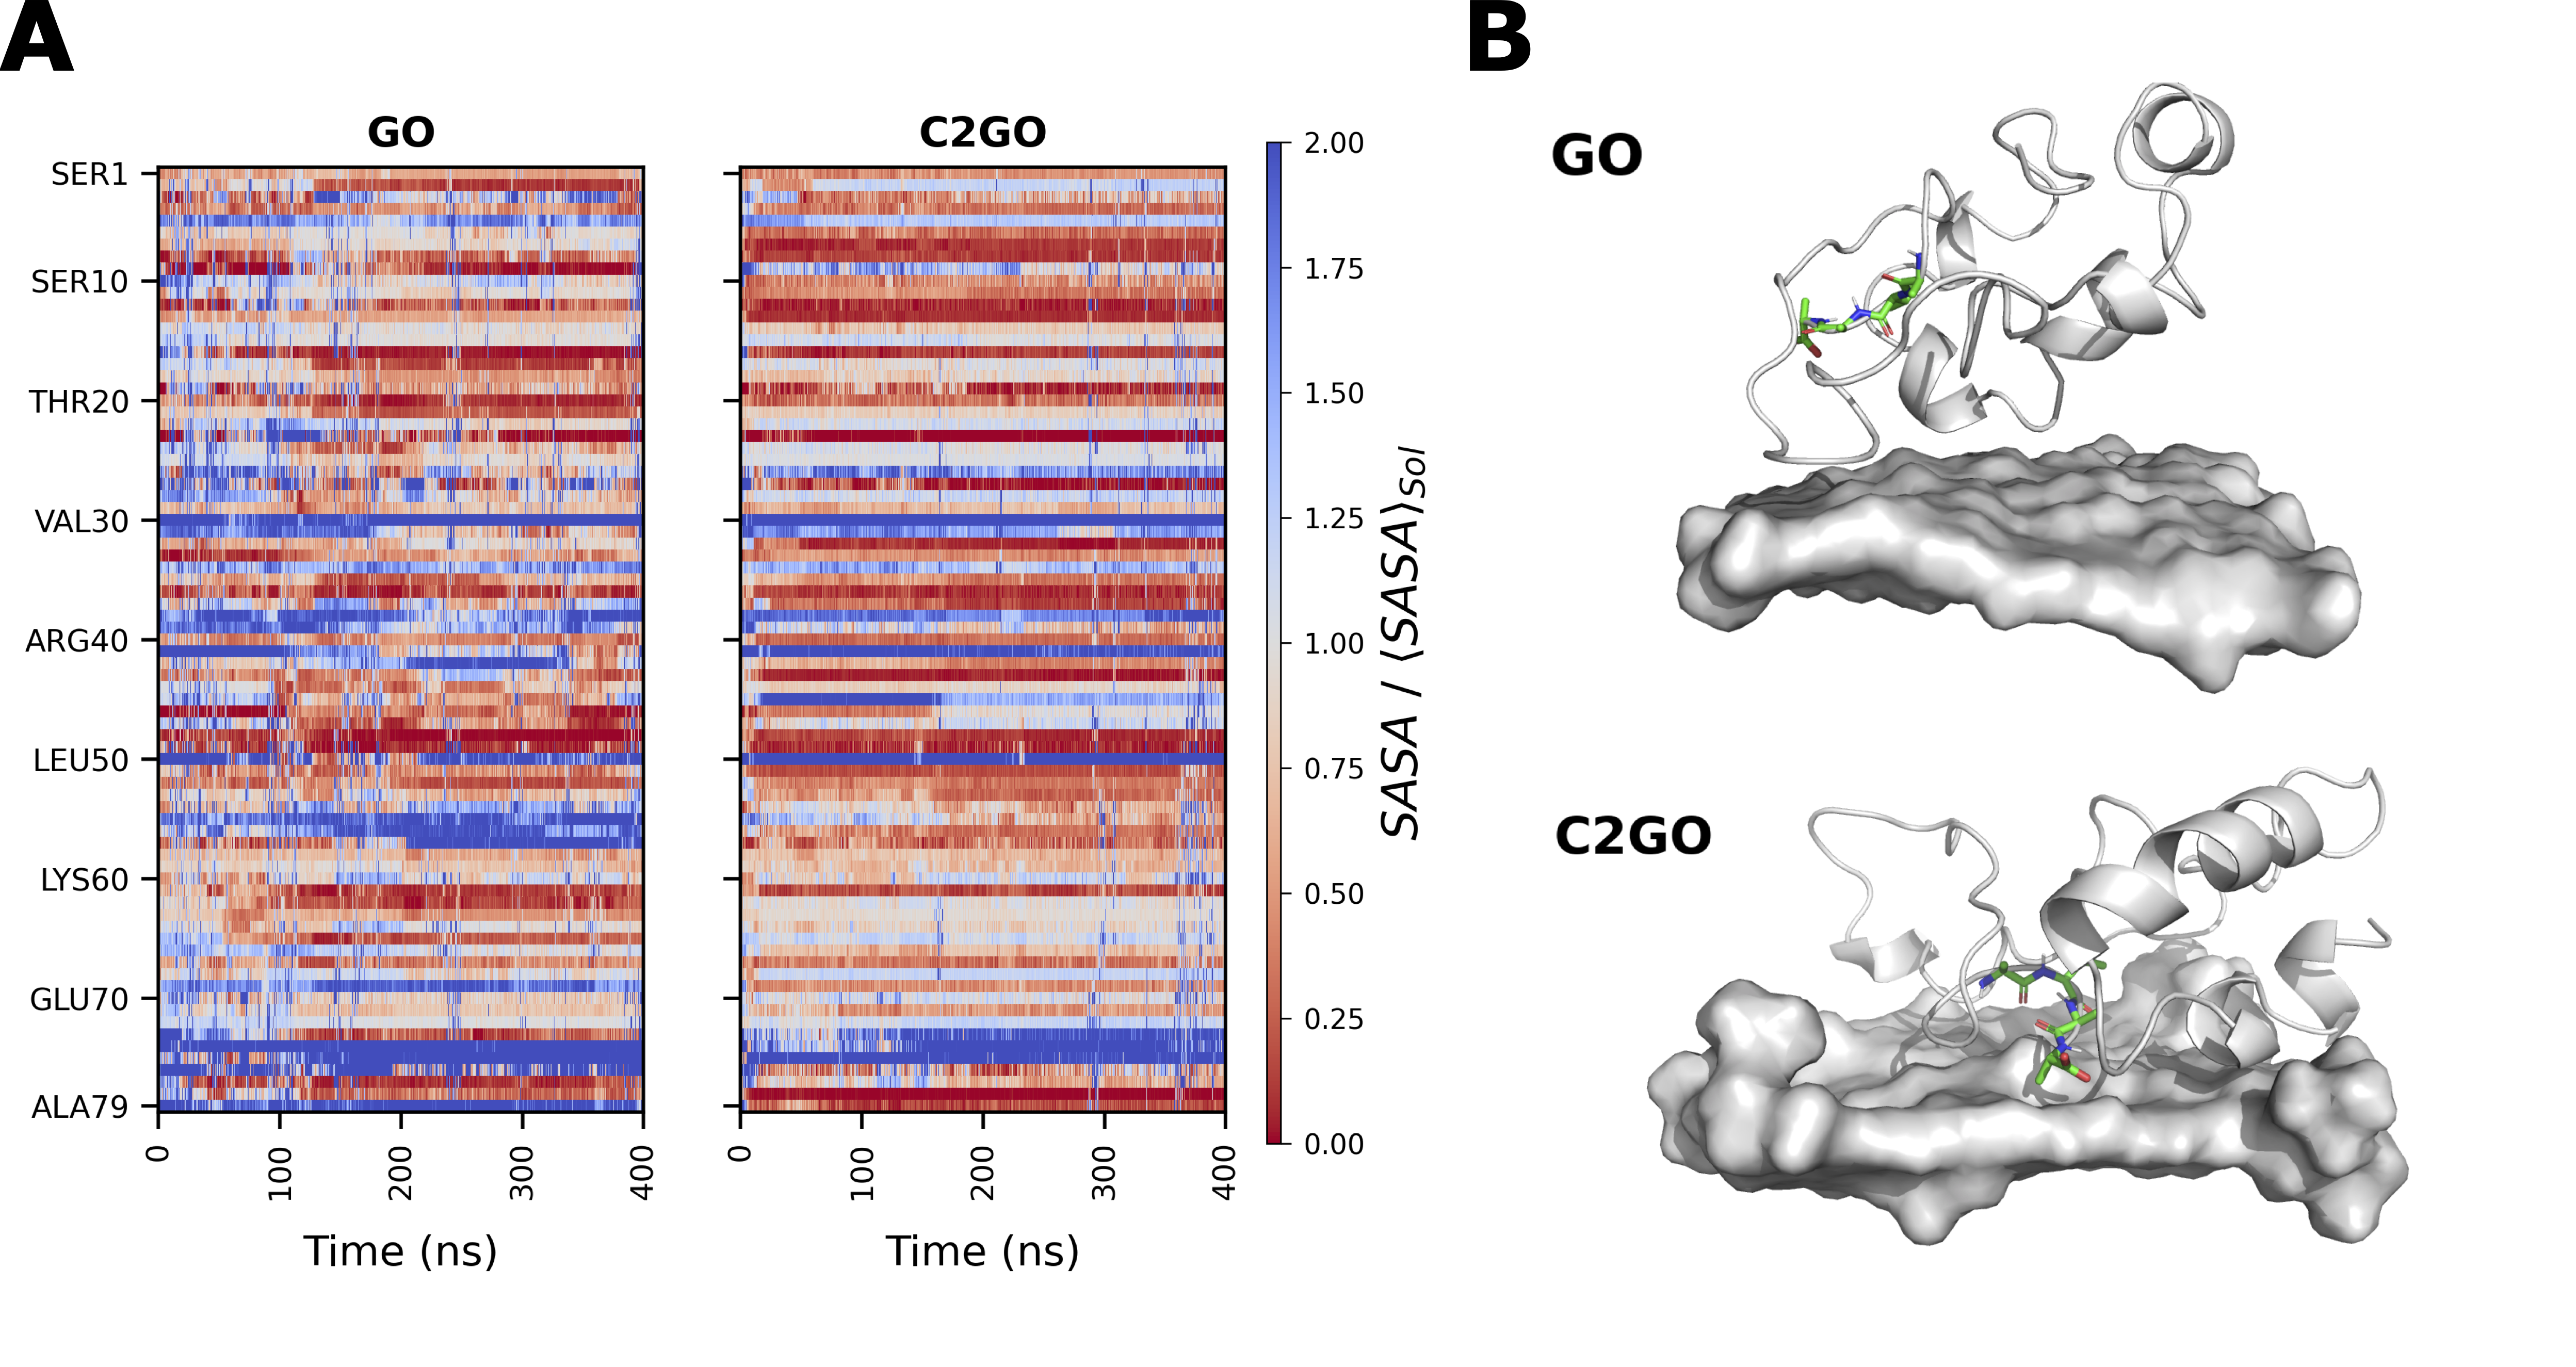
\includegraphics[width=\textwidth]{sasa-snapshot.png}
    \caption{The surface accessible surface area (SASA) of apo-c3 amino acid residues during adsorption to GO and C2GO sheets, normalised by average SASA of apo-c3 in solution (A) and illustration of exposure of the AVAA minimotif in the C-terminal region of apo-c3 to solvent in GO adsorption and contrasting structure in C2GO adsorption, the nanomaterials are represented as a surface for clarity (B).}
    \label{fig:sasa}
\end{figure*}

Previous work has found that the C-terminal region of apo-c3 is essential for mediating lipid binding, with the N-terminal region (residues 1-40) playing a limited secondary role.\cite{sparrow1977lipid, meyers2017aromatic, lambert1996effect} Solvent exposure analysis of the C-terminal helix expresses the conservation of its lipid-binding function from a physio-chemical perspective. These results may in part delineate the experimentally observed preferential uptake of corona-coated C2GO to corona-coated GO by J774 cells.\cite{mei2018protein} 
%--------------------------------------
%               METHODS 
%--------------------------------------
\section{Methods}
\subsection{Nanomaterial structure}
%
We have modified a Python package \cite{make-graphitics-github} to generate azide and trimethylsilyl (TMS)-alkyne functional group conjugated rectangular graphene-oxide flakes.\cite{albadri2020accurate-github} The package improves on the commonly applied protocol, of randomly placing oxidised functional groups, which we now know is an incomplete model of graphene-oxide structure.\cite{al2020accurate, mouhat2020structure} Instead, we recreate the two-phase nature of oxidised and unoxidised graphene domains observed in microscopy experiments \cite{Pacile2011, Cai2008, Saxena2010, Erickson2010} in accordance with our recent study of accurate large scale modelling of graphene oxide.\cite{al2020accurate}
\subsection{Molecular Dynamics}
%
MD simulations were performed in GROMACS version 2020.1 on the ARCHER2 AMD EPYC Zen2 (Rome) 64 core CPUs at 2.2 GHz or Nvidia V100 GPUs. The all-atom OPLS forcefield was used to simulate the classical simulations. A position restraint algorithm was applied to all non-solvent atoms during equilibration. The $\sim$130\,\AA\, cubic simulation box was fully solvated with TIP3P water molecules. The system net charge was neutralised by adding four sodium ions into the system. The system was relaxed energetically using steepest-descent energy minimisation for 50000 steps with an energetic step size of 0.01 kJ/mol. The minimisation was terminated after the maximum energetic contribution was lower than a threshold of 1000.0 kJ/mol/nm. NVT and NPT equilibration was performed for 100 ps using two separate modified velocity-rescaling thermostat --- with a stochastic term to ensure generating the canonical ensemble --- coupling temperature to velocities for graphene and solvent molecules (NVT),\cite{bussi2007canonical} where a temperature of 300K was maintained and 1 bar using the Parrinello-Rahman barostat (NPT). The Verlet cut-off scheme was employed to generate pair lists and the electrostatic interactions were calculated using the Particle-Mesh Ewald algorithm. Both electrostatic and van der Waals interactions were cut off beyond 1.2 nm. All bonds involving hydrogen atoms were constrained using the LINCS algorithm. Production simulations were run for 400 ns using a timestep of 1~fs. Analysis was performed using the MDAnalysis package \cite{mda, oliver_beckstein-proc-scipy-2016, Michaud-Agrawal-2011} and its analysis modules.\cite{araya2014characterization,smith2019interaction} To identify hydrogen bonds we used the hydrogen bond analysis tool \cite{smith2019interaction} implemented
in MDAnalysis. We used the MDTraj \cite{McGibbon2015MDTraj} implementation of DSSP. 

\subsection{Contact maps}
Contact maps between apo-c3 and the graphitic sheets were calculated using a hard cutoff of \SI{5.0}{\angstrom} between any two heavy (non-hydrogen) atoms. Data over the final \SI{50}{\nano\second} were used for the contact maps, as during this period apo-c3 was stably adsorbed to both GO and C2GO. We constructed contact maps between between GO/C2GO and each specific residue of apo-c3 (Fig.~\ref{fig:prot-go-contacts} and \ref{fig:prot-c2go-contacts}), as well as contact maps between GO/C2GO and each amino acid regardless of its position in the sequence (Fig.~\ref{fig:contacts}B).
%
\subsection{PBSA binding energies}
We post process the last \SI{10}{\nano\second} of MD trajectories using molecular mechanics with Poisson–Boltzmann and surface area solvation (MM-PBSA) analysis implemented using g\_mmpbsa,\cite{kumari2014g_mmpbsa} to obtain a relative order of binding of apo-c3 to the different graphitic nanosheets. The energetic components of the binding free energy are the changes in the system potential energy \textit{in vacuo}, the polar and non-polar solvation energies. The potential energy accounts for bonded (bond, angle and torsion) and non-bonded (van der Waals and electrostatic) energetic terms. Polar solvation energy is the electrostatic contribution to the solvation free energy and is estimated using the Poisson-Boltzmann equation. The non-electrostatic contribution to the solvation free energy accounts for forces between solute and solvent, which are calculated using the solvent accessible surface area (SASA).\cite{kumari2014g_mmpbsa} 
%
\subsection{UMAP dimensionality reduction}
We used the atomic coordinates of apo-c3 to obtain an ensemble of distinct structural conformations when adsorbed to the graphitic sheets. We first centre and align the structures along their backbone atoms, using every tenth frame (\SI{50}{\pico\second}) from the trajectory. We then use the uniform manifold approximation and projection for dimension reduction (UMAP\cite{mcinnes2018umap-software}) algorithm to embed the atomic coordinates of heavy atoms of apo-c3 into a two-dimensional space. UMAP constructs a graph of the points in the high-dimensional space, then optimises a low-dimensional representation of the graph such that the topological distance is preserved to a degree in the embedding.\cite{mcinnes2018umap-software} Therefore, similar conformations that are close in the high-dimensional space will also be close in the reduced space. We set the \code{n\_neighbours} and \code{min\_dist} hyperparameters to 15 and 0.0, respectively, with the latter being a requirement if the points in the reduced space are to be clustered. We use HDBSCAN\cite{mcinnes2017hdbscan}, implemented in scikit-learn\cite{scikit-learn}, to cluster the apo-c3 conformations in the embedded space. We identify representative structures of each conformation by calculating the mean structure of a conformation, then finding the structure with the smallest RSMD from this mean structure.
%
\subsection{SASA solvent exposure}
To quantify the solvent exposure of amino acids during adsorption, we calculated the solvent accessible surface area of each residue of apo-c3 over time. To understand how the conformational changes lead to exposure of residues that are buried in the native state, we normalised the SASA time-series by the mean SASA of each residue of the protein in solution. We used the final \SI{50}{\nano\second} of apo-c3 solution for determining the mean SASA of each residue. Values greater than and less than \num{1} indicate, respectively, increased and decreased exposure to the solvent (Fig.~\ref{fig:sasa}A). The SASA was calculated using the ``rolling-ball" Shake-Rupley algorithm,\cite{SHRAKE1973} implemented in MDTraj.\cite{McGibbon2015MDTraj} This approximates the SASA by effectively rolling a ball over each atom of the protein to define a surface, then examining how much of the each atom's surface is exposed to solvent as opposed to overlapping with surfaces of neighbouring atoms. The radius of the probe in typically set to \SI{1.4}{\angstrom} --- approximately the radius of a water molecule.


%--------------------------------------
%             CONCLUSIONS 
%--------------------------------------
\section{Conclusions}

 This work has dissected the protein structural changes induced by interactions of functional groups and protein residues on the bio-nano interface. Through adsorption on GO, apo-c3 shows denaturing of the secondary structure over large swathes of the protein sequence. Whereas C2GO-adsorbed apo-c3 has limited deformation, with most variance displayed in the N-terminus. The C-terminus of apo-c3 has previously been found to be responsible for lipid binding, with the N-terminus playing a limited secondary role.\cite{sparrow1977lipid, meyers2017aromatic, lambert1996effect} These findings correlate with experimental evidence of the increased cellular uptake of C2GO, as compared to GO, hard protein corona.\cite{mei2018protein} \\

Apo-c3 is found to denature upon adsorption to GO, according to solvent exposure, DSSP and conformational clustering analyses. Following adsorption on GO, apo-c3 forms 3 separate $\beta$-turns that serve as binding motifs for protein-protein interactions. These can aid in subsequent aggregation of serum proteins to the corona, contributing to the corona identity in vivo, hence complicating the targetability of the nanomaterial-corona complex. \\

The functional groups at the binding interface between the nanomaterials and apo-c3 set off a series of dynamic events that result in large-scale secondary structure changes. Contact distances, heatmaps and binding free energy calculations collectively describe the driving forces of the changes in protein structure following adsorption. The introduction of azide and TMS functional groups was sufficient to stop the denaturing of apo-c3 and the formation of $\beta$-turns that serve as protein-protein interaction binding motifs. We find that contact with azide functional groups correlate strongly with contact to other surface functional groups and therefore work cooperatively to maximise the binding surface at the bio-nano interface. Consequently, the C2GO-adsorbed protein is stabilised and is not pushed to structural deformation as is the case in GO-adsorbed protein. The results from this analysis pipeline suggest the causes of protein aggregation and cellular uptake are mediated by the aforementioned changes in protein structure. \\

This work indicates that the dynamic and functional role of adsorbed proteins may be a more important probe to understanding the protein corona, rather than quantifying a static image of its constituent proteins. MD simulations are a valuable tool for such an investigation and our analysis pipeline serves as a transferable method for understanding the structure/function relationship of dynamic protein-nanomaterial adsorption.

%Analysis methods are outlined in the SI, including contact maps (Supp. Note 1), MM-PBSA binding energy calculations\cite{kumari2014g_mmpbsa} (Supp. Note 2), UMAP dimensionality reduction\cite{mcinnes2017hdbscan, scikit-learn} and HDBSCAN clustering\cite{mcinnes2017hdbscan} (Supp. Note 3) and SASA solvent exposure\cite{SHRAKE1973, McGibbon2015MDTraj} (Supp. Note 4).
%\section*{Supplementary figures}
%
\begin{figure}[ht!]
    \centering
    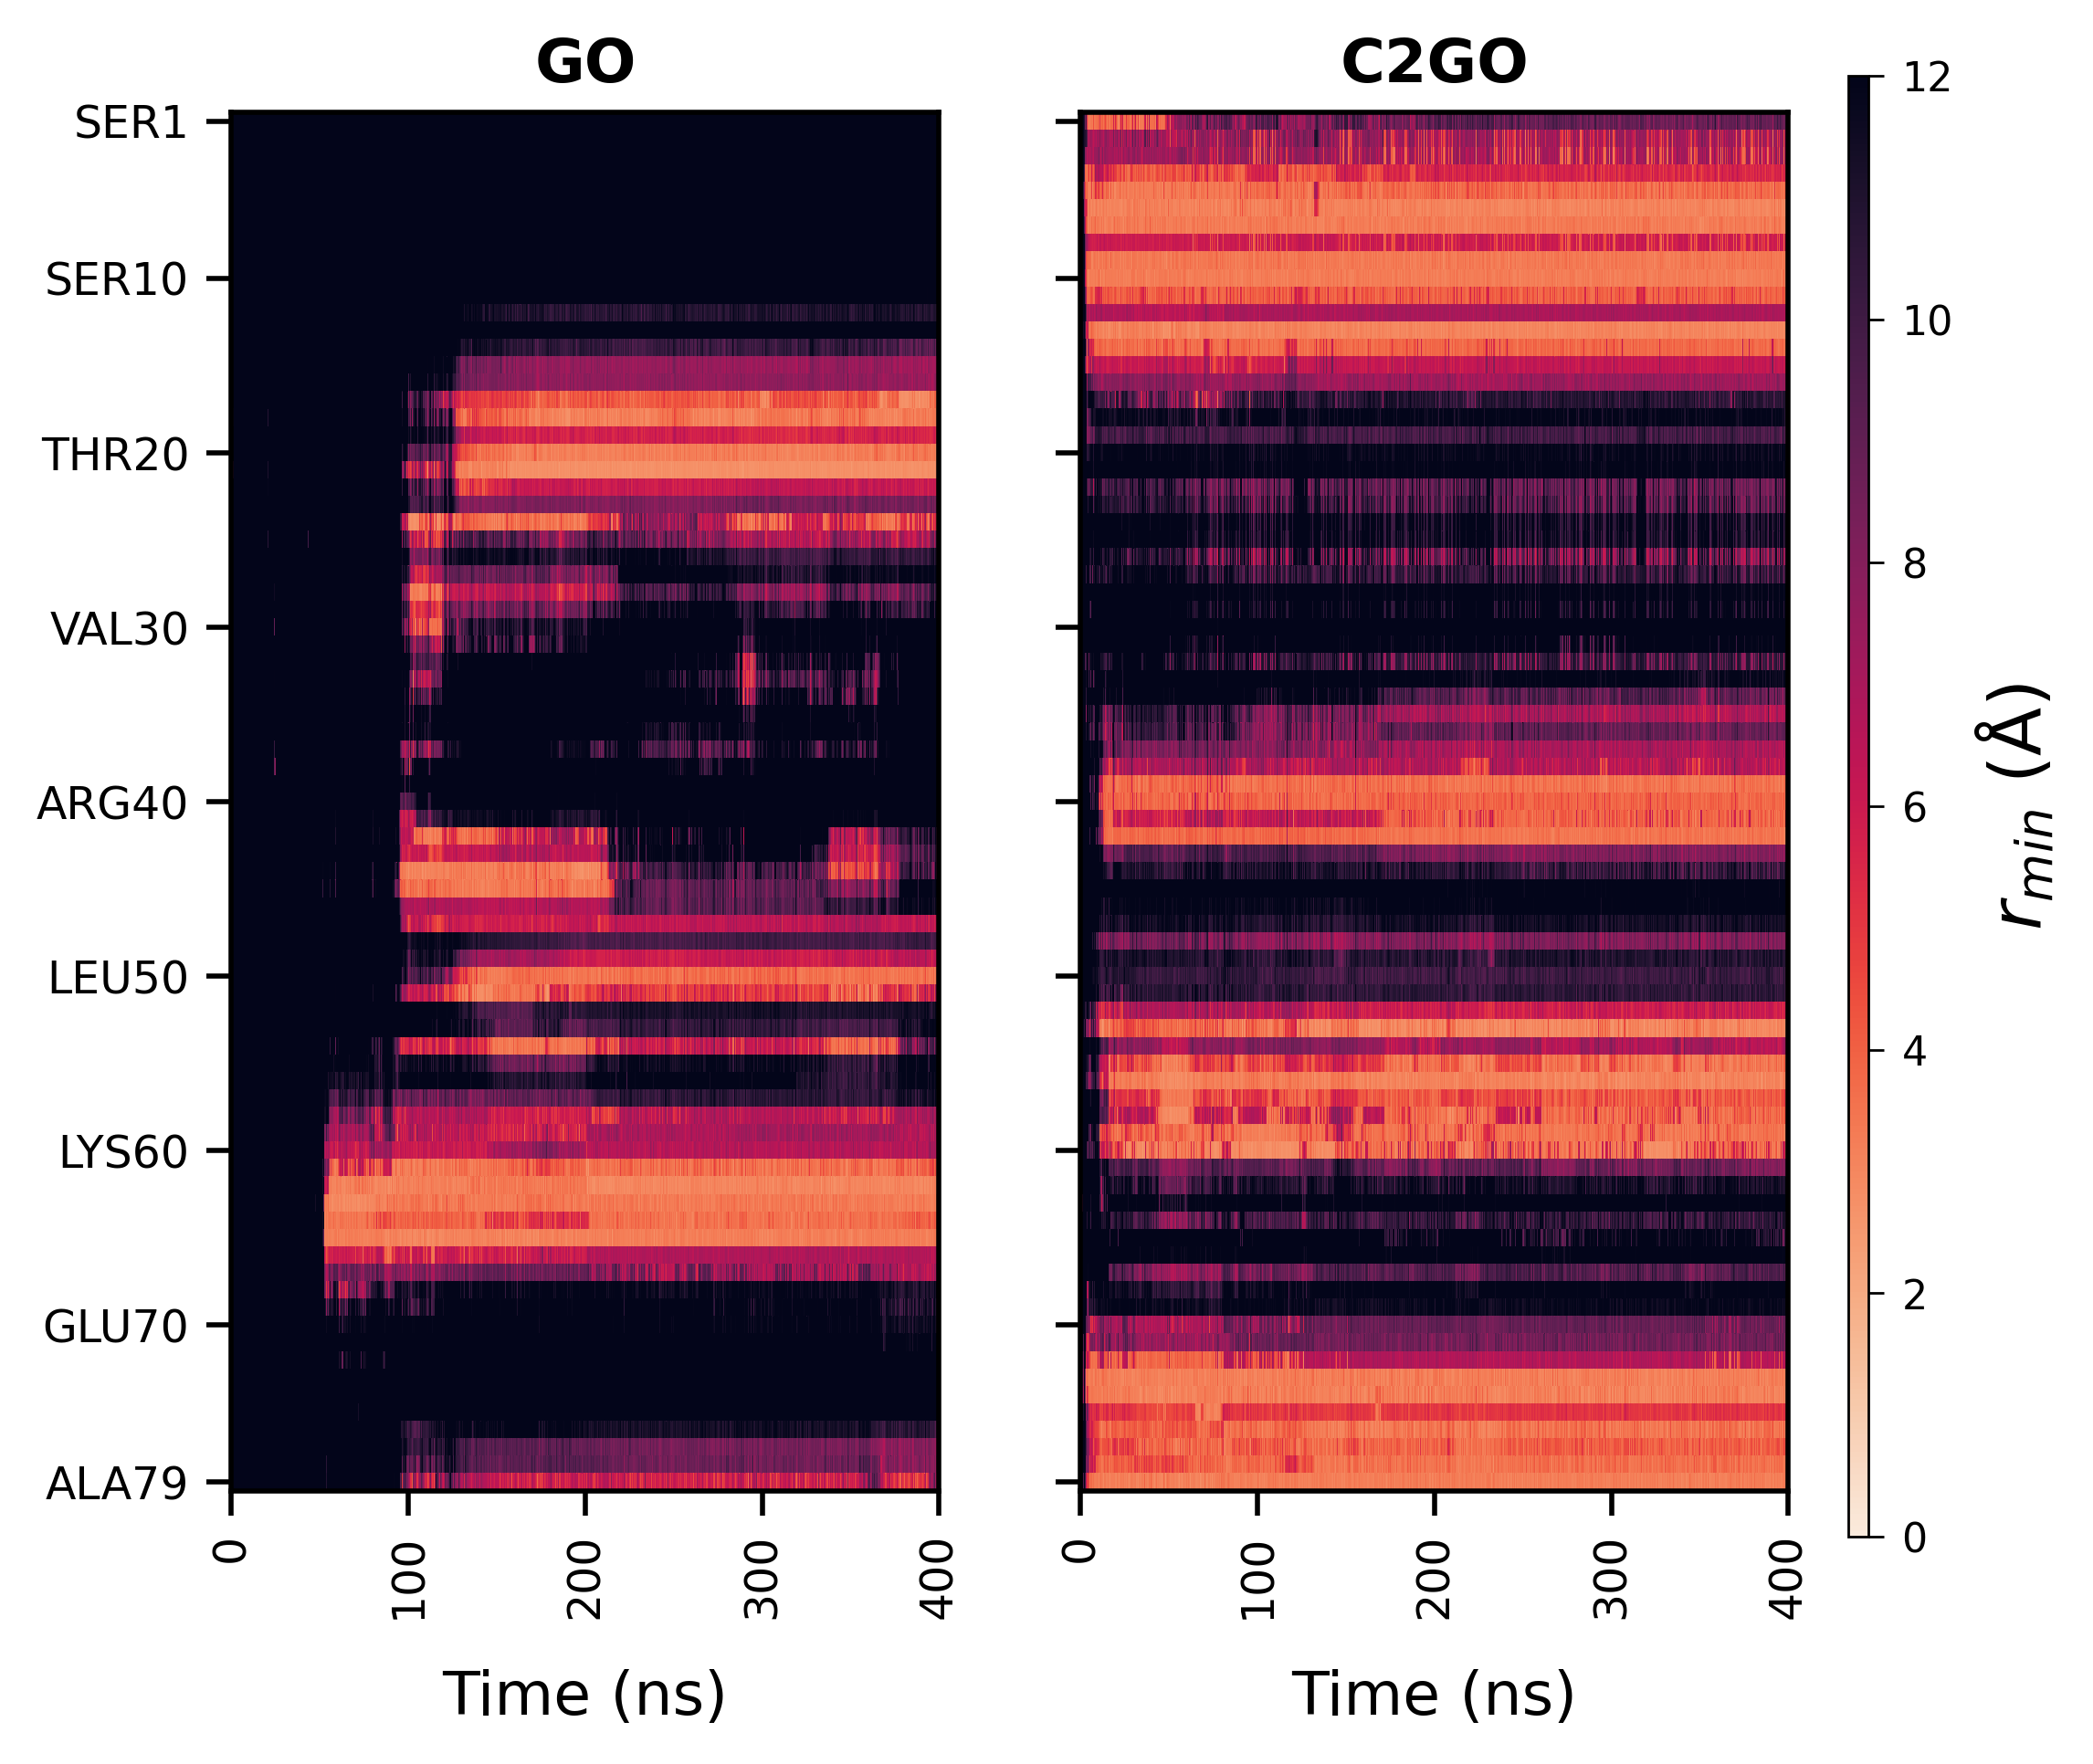
\includegraphics[width=0.8\linewidth]{SI_min-dist-to-grap.png}
    \caption{Minimum distance to any GO/C2GO heavy atom for each residue in apo-C3.}
    \label{fig:mid-dist-to-grap}
\end{figure}

\begin{figure}
    \centering
    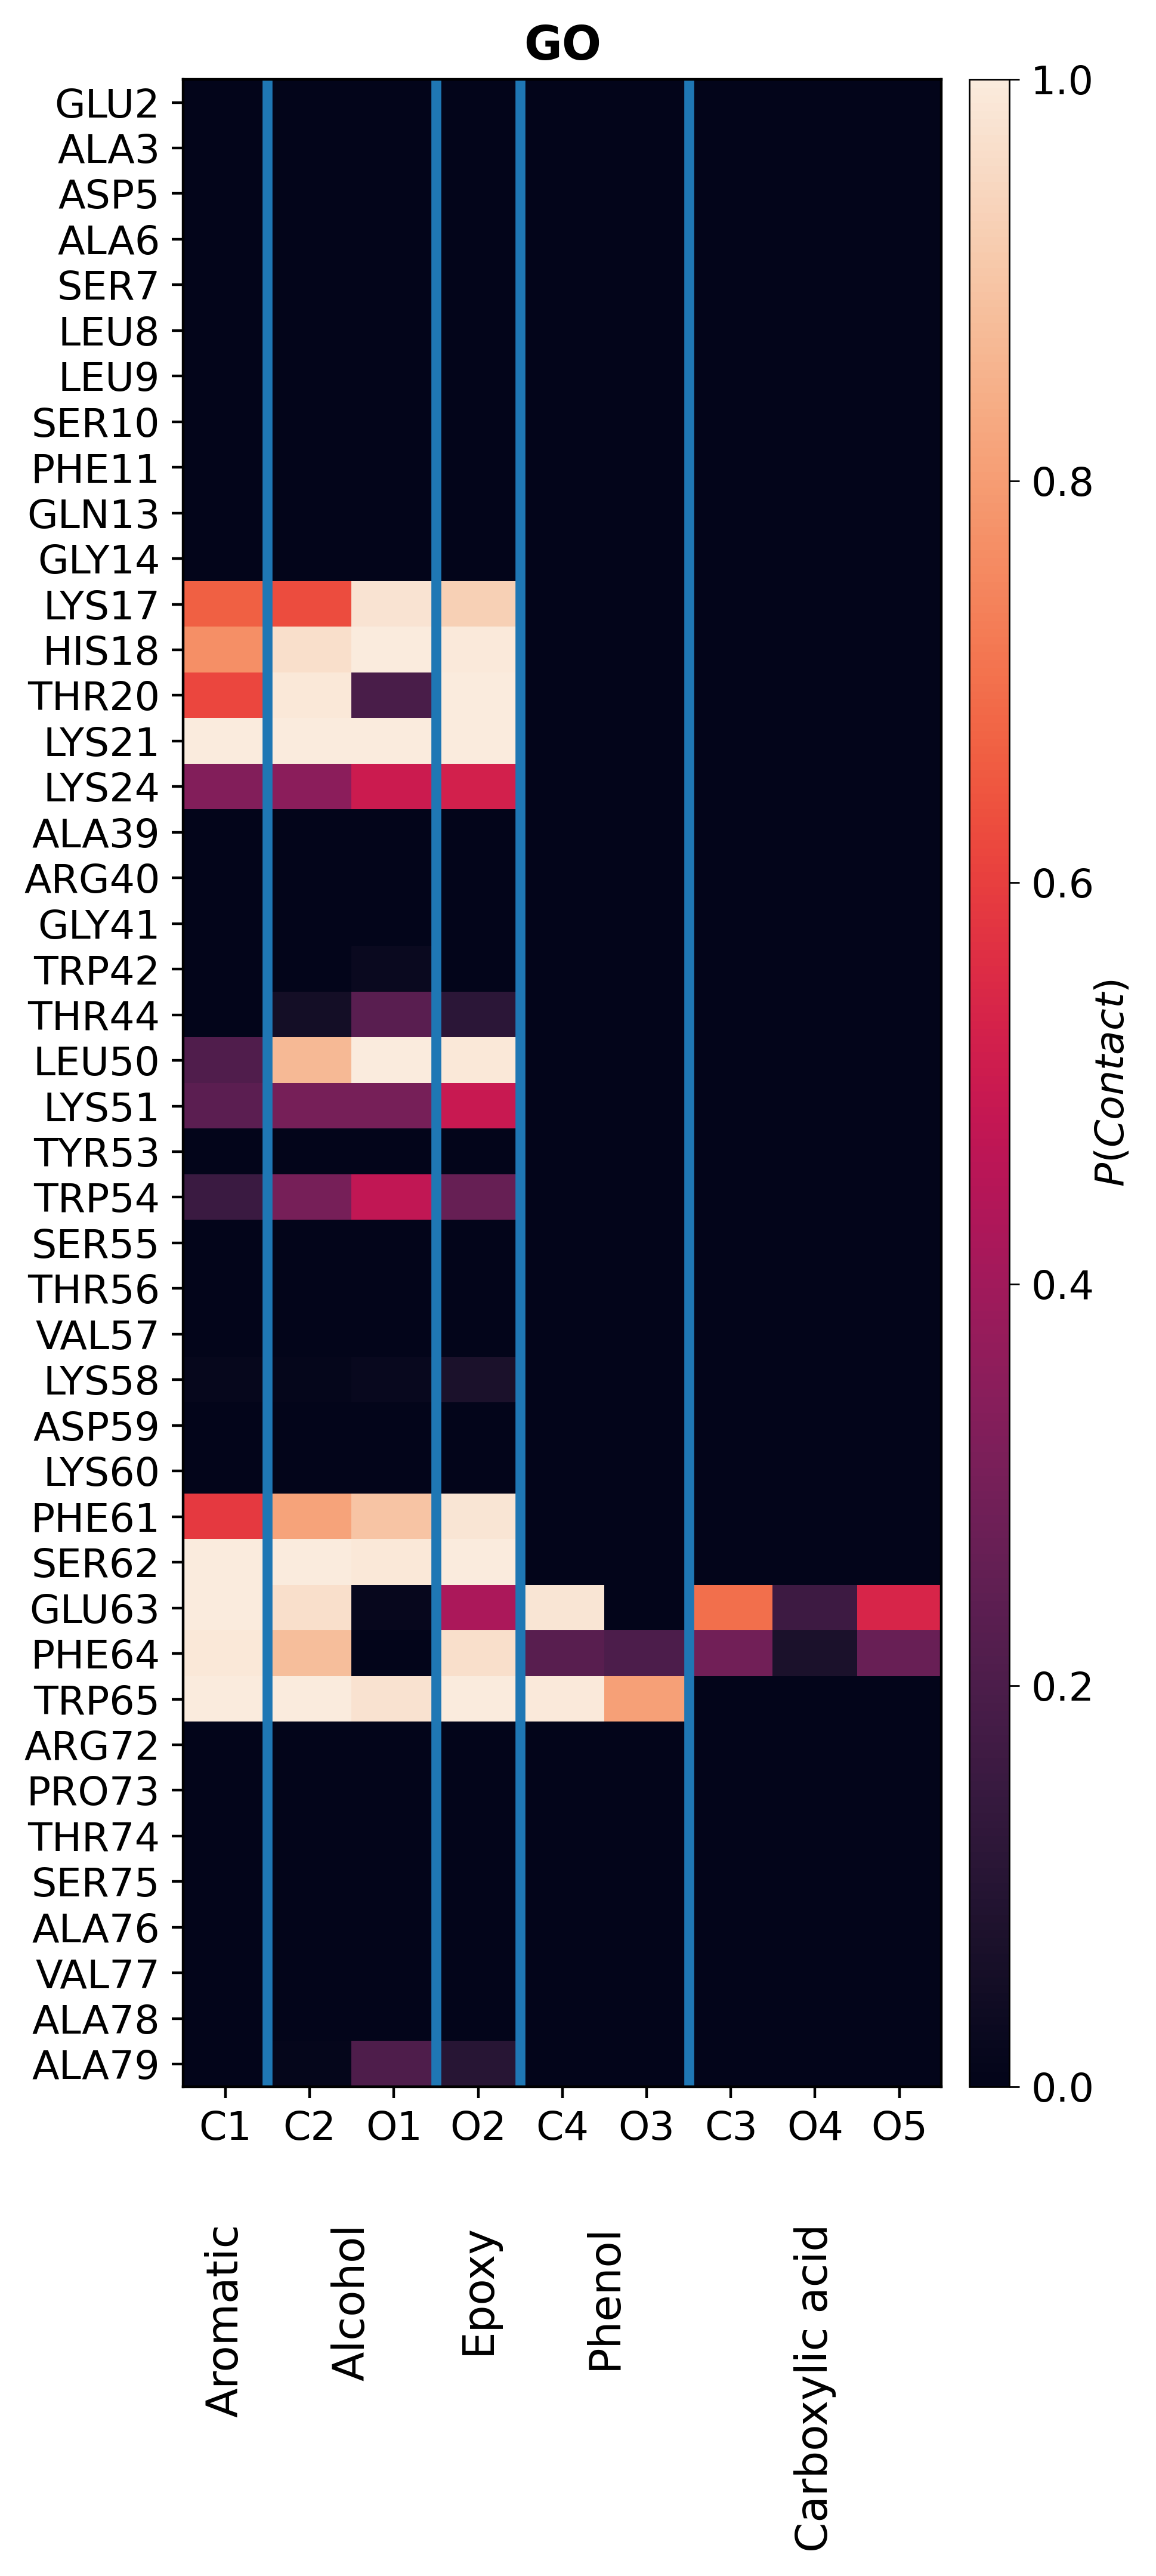
\includegraphics[height=18cm]{SI_go-OPLS-R1-residues-condensed_P01.png}
    \caption{Contact probability between each apo-C3 residue and each atom type of GO. Data from the final \SI{50}{\nano\second} of the trajectory. For clarity, only those residues with $P(\mathrm{Contact}) \geq 0.1$ for either GO or C2GO are shown.}
    \label{fig:prot-go-contacts}
\end{figure}

\begin{figure}
    \centering
    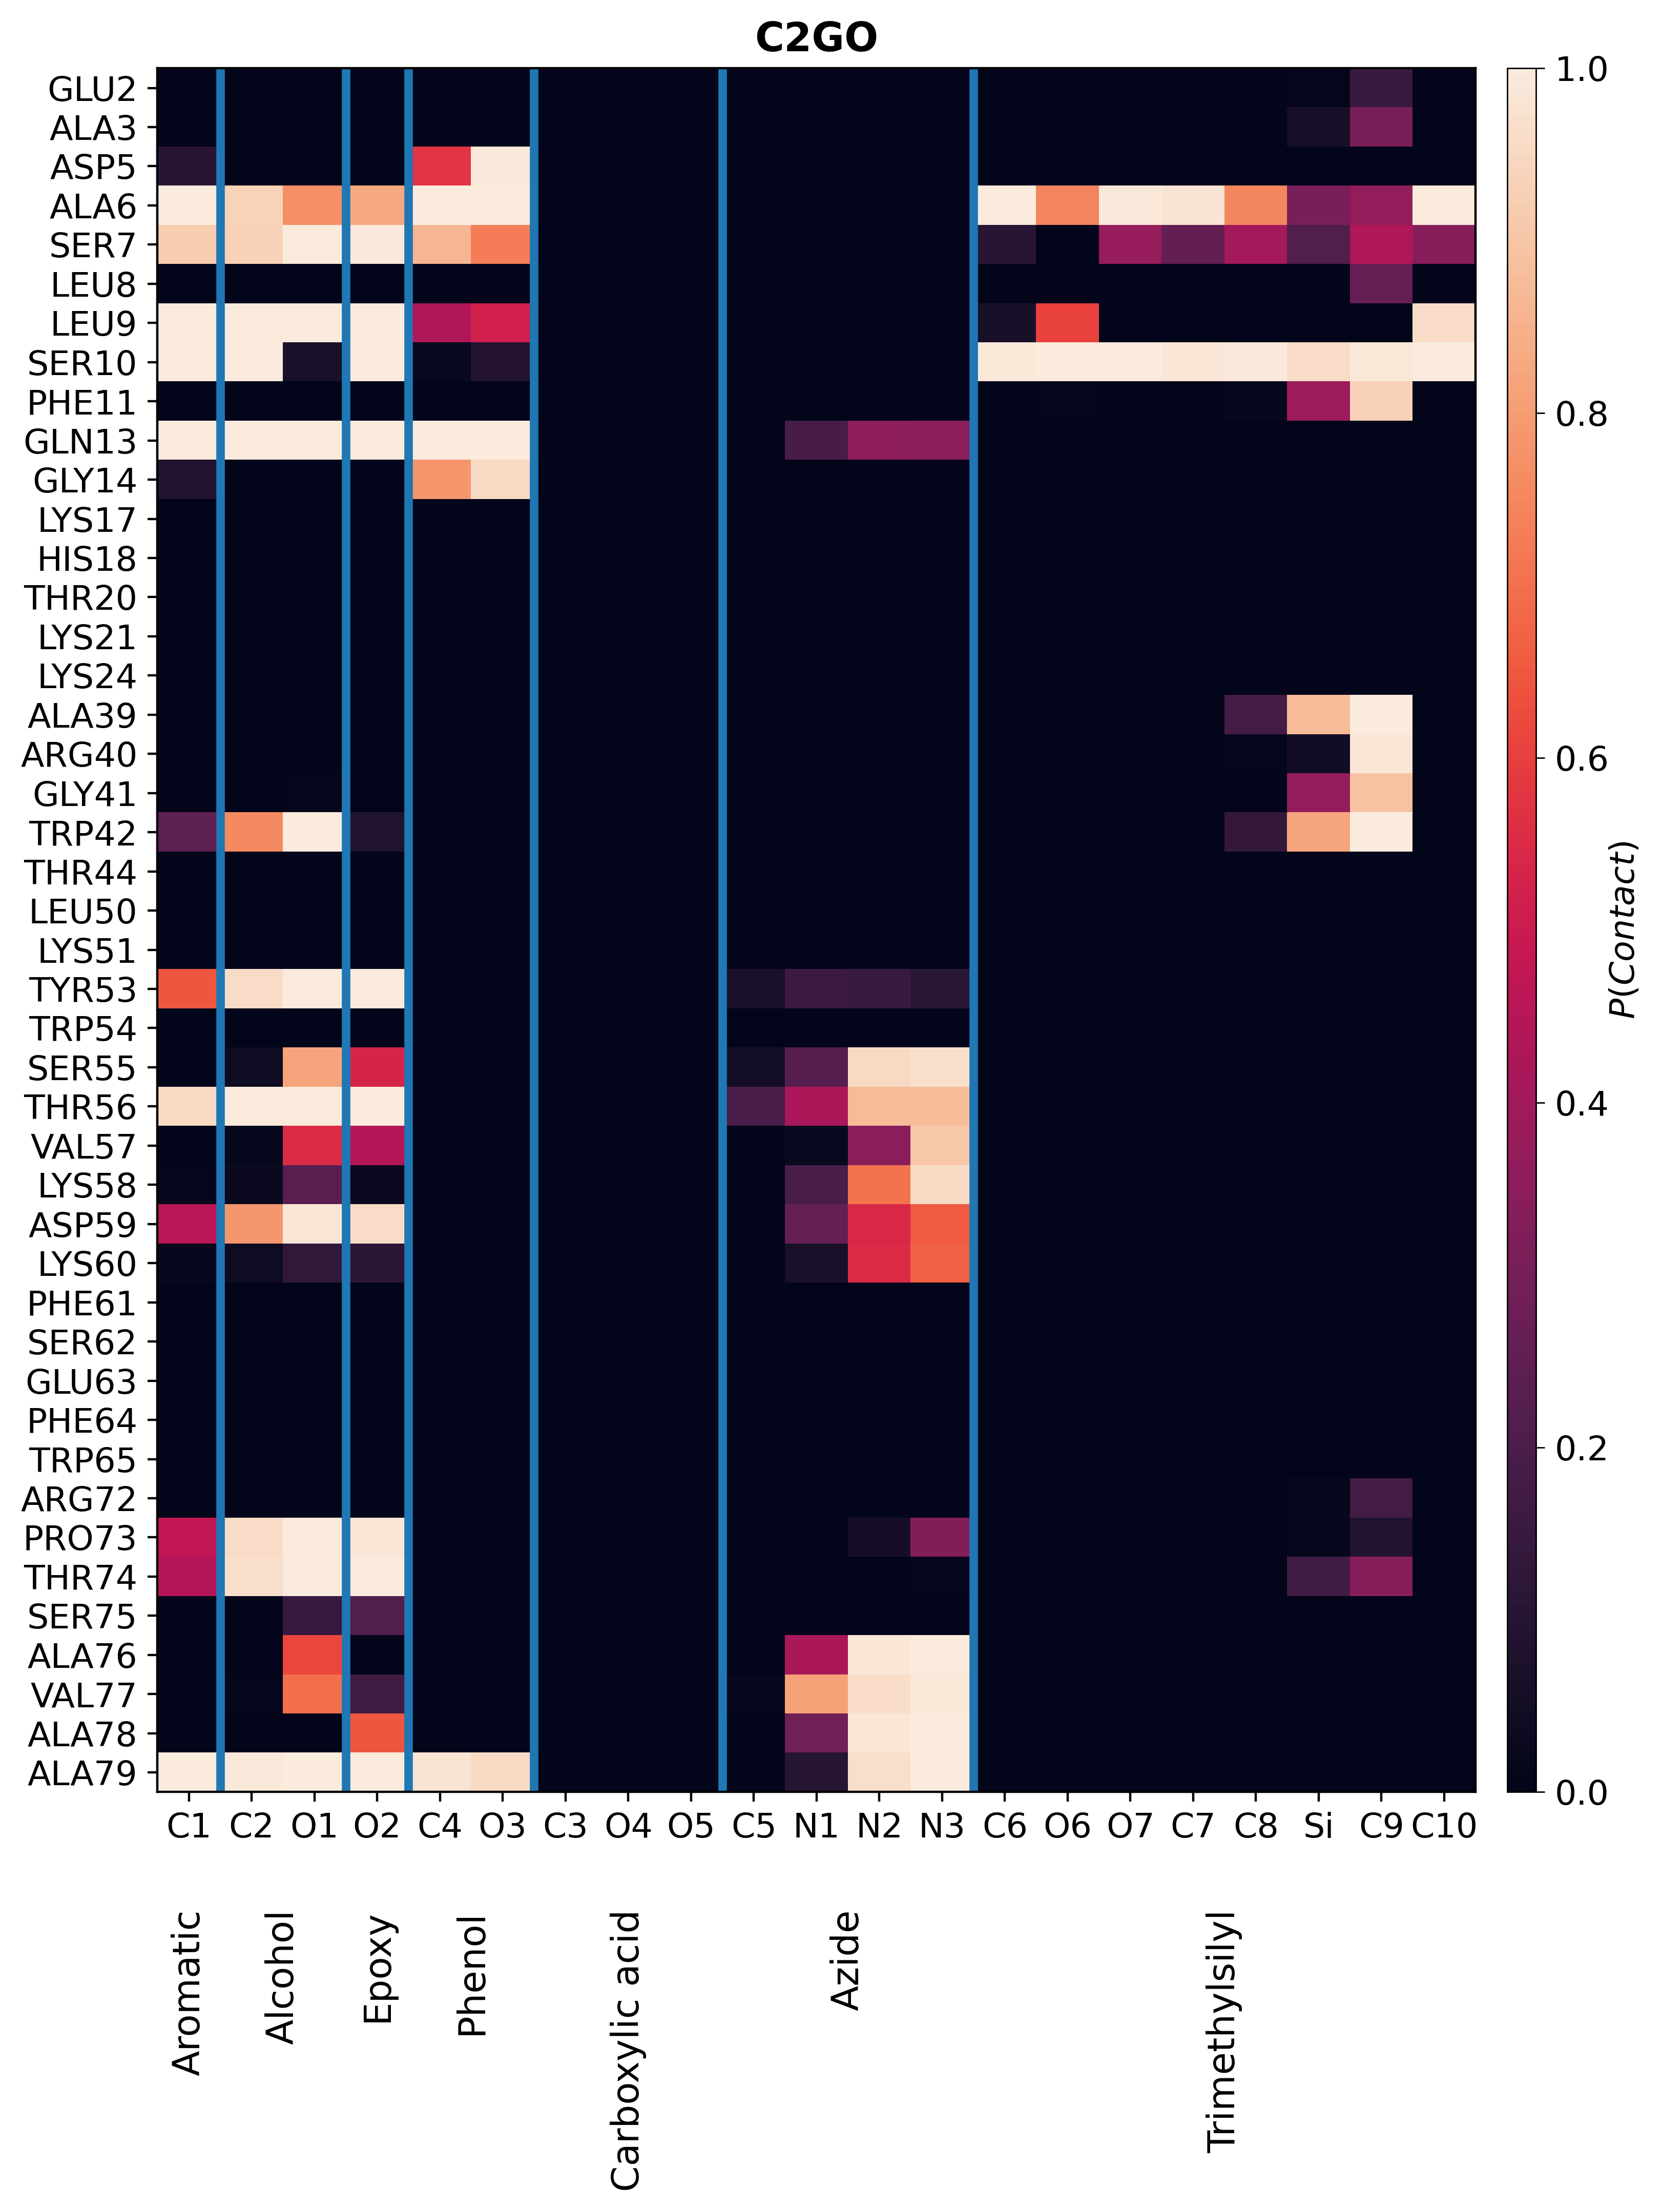
\includegraphics[height=18cm]{SI_c2go-OPLS-R2-residues-condensed_P01.png}
    \caption{Contact probability between each apo-C3 residue and each atom type of C2GO. Data from the final \SI{50}{\nano\second} of the trajectory. For clarity, only those residues with $P(\mathrm{Contact}) \geq 0.1$ for either GO or C2GO are shown.}
    \label{fig:prot-c2go-contacts}
\end{figure}

% \chapter{Exploring bifurcations between phenotypes}
\label{chapter:exploring}

% \vspace{-1cm}
\chapter{Superexchange mechanism and quantum manybody excitations in the archetypal di-Cu oxo-bridge}
\label{Hemocyanin}
\vspace{-1cm}

In this work, we study the electronic structure of the hemocyanin protein, where in particular we study the 59-atom protein core using density functional theory + dynamical mean field theory (DFT+DMFT). Here, we find that the hemocyanin protein utilises electronic correlation effects in performing its function of oxygen transport. By treating the copper 3\textit{d} electrons in the hemocyanin functional site using DMFT, we recover experimentally observed singlet electronic ground state. This work allows the transferability of the DFT+DMFT approach to the quantum treatment of the entire protein, using linear-scaling DFT. The importance of accurate simulation of the Hemocyanin core is in understanding how biological systems have evolved to function through quantum biology, as well as its use in biomimetic applications in engineering.\cite{al2020superexchange} \edit{Contributions for this work are as follows: \textbf{Cedric Weber} and \textbf{Mohamed Ali al-Badri} conceived and planned the research. \textbf{Mohamed Ali al-Badri, Edward Linscott} and \textbf{Cedric Weber} performed the calculations. \textbf{Mohamed Ali al-Badri
Edward Linscott, Antoine Georges, Daniel J. Cole} and \textbf{Cedric Weber} analysed the data and contributed to the final manuscript. \textbf{Edward Linscott} independently ran the NBO analysis (Supp. Fig.~3) and the scaling calculations (Supp. Fig.~5).}

%Contributions for this work are as follows: \textbf{Cedric Weber and Mohamed Ali al-Badri} conceived and planned the research. \textbf{Mohamed Ali al-Badri, Edward Linscott} and \textbf{Cedric Weber} performed the calculations. \textbf{Mohamed Ali al-Badri, Edward Linscott, Antoine Georges, Daniel J. Cole} and \textbf{Cedric Weber} analysed the data and contributed to the final manuscript. \edit{Edward Linscott independently ran the Natural Bonding Orbital (NBO) analysis (Supplementary Fig.~3) and the scaling calculations (Supplementary Fig.~5).}
%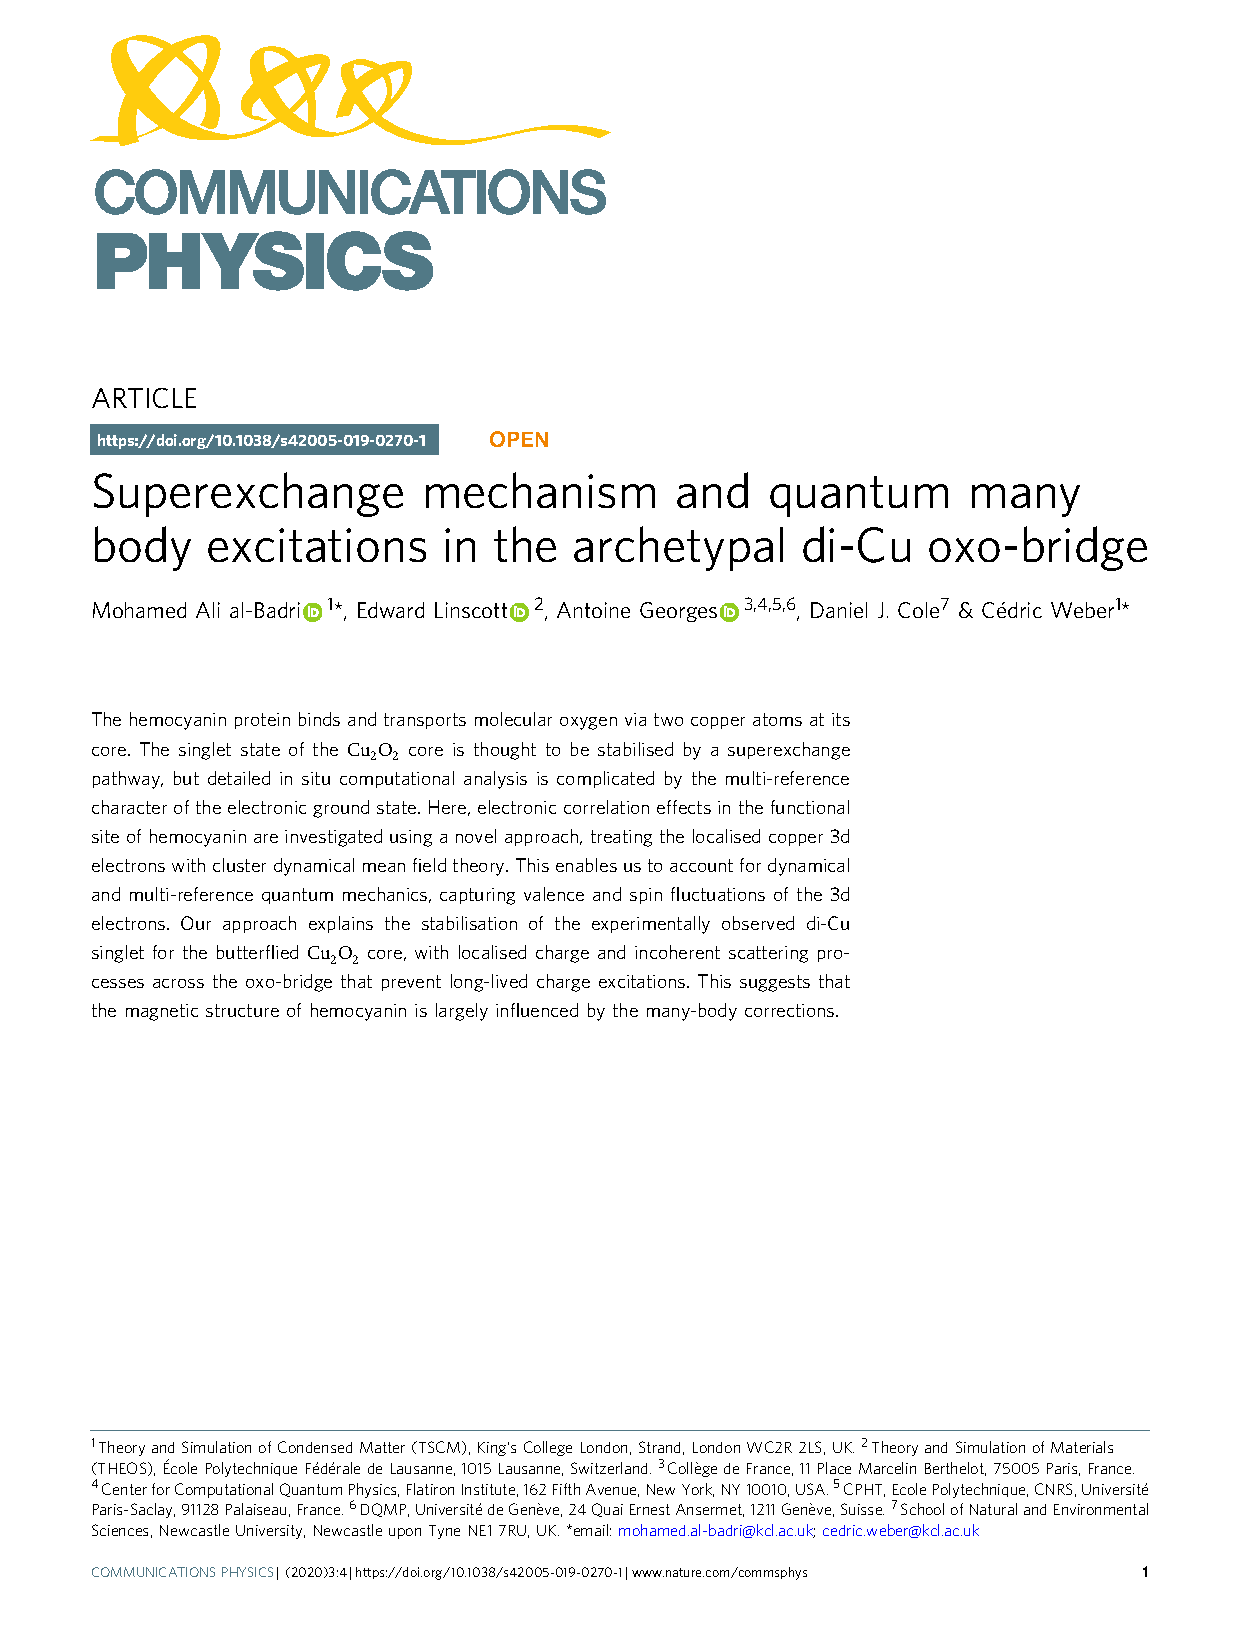
\includepdf[pages=-, offset=75 -75]{PDF_PAPERS/hemocyanin.pdf}


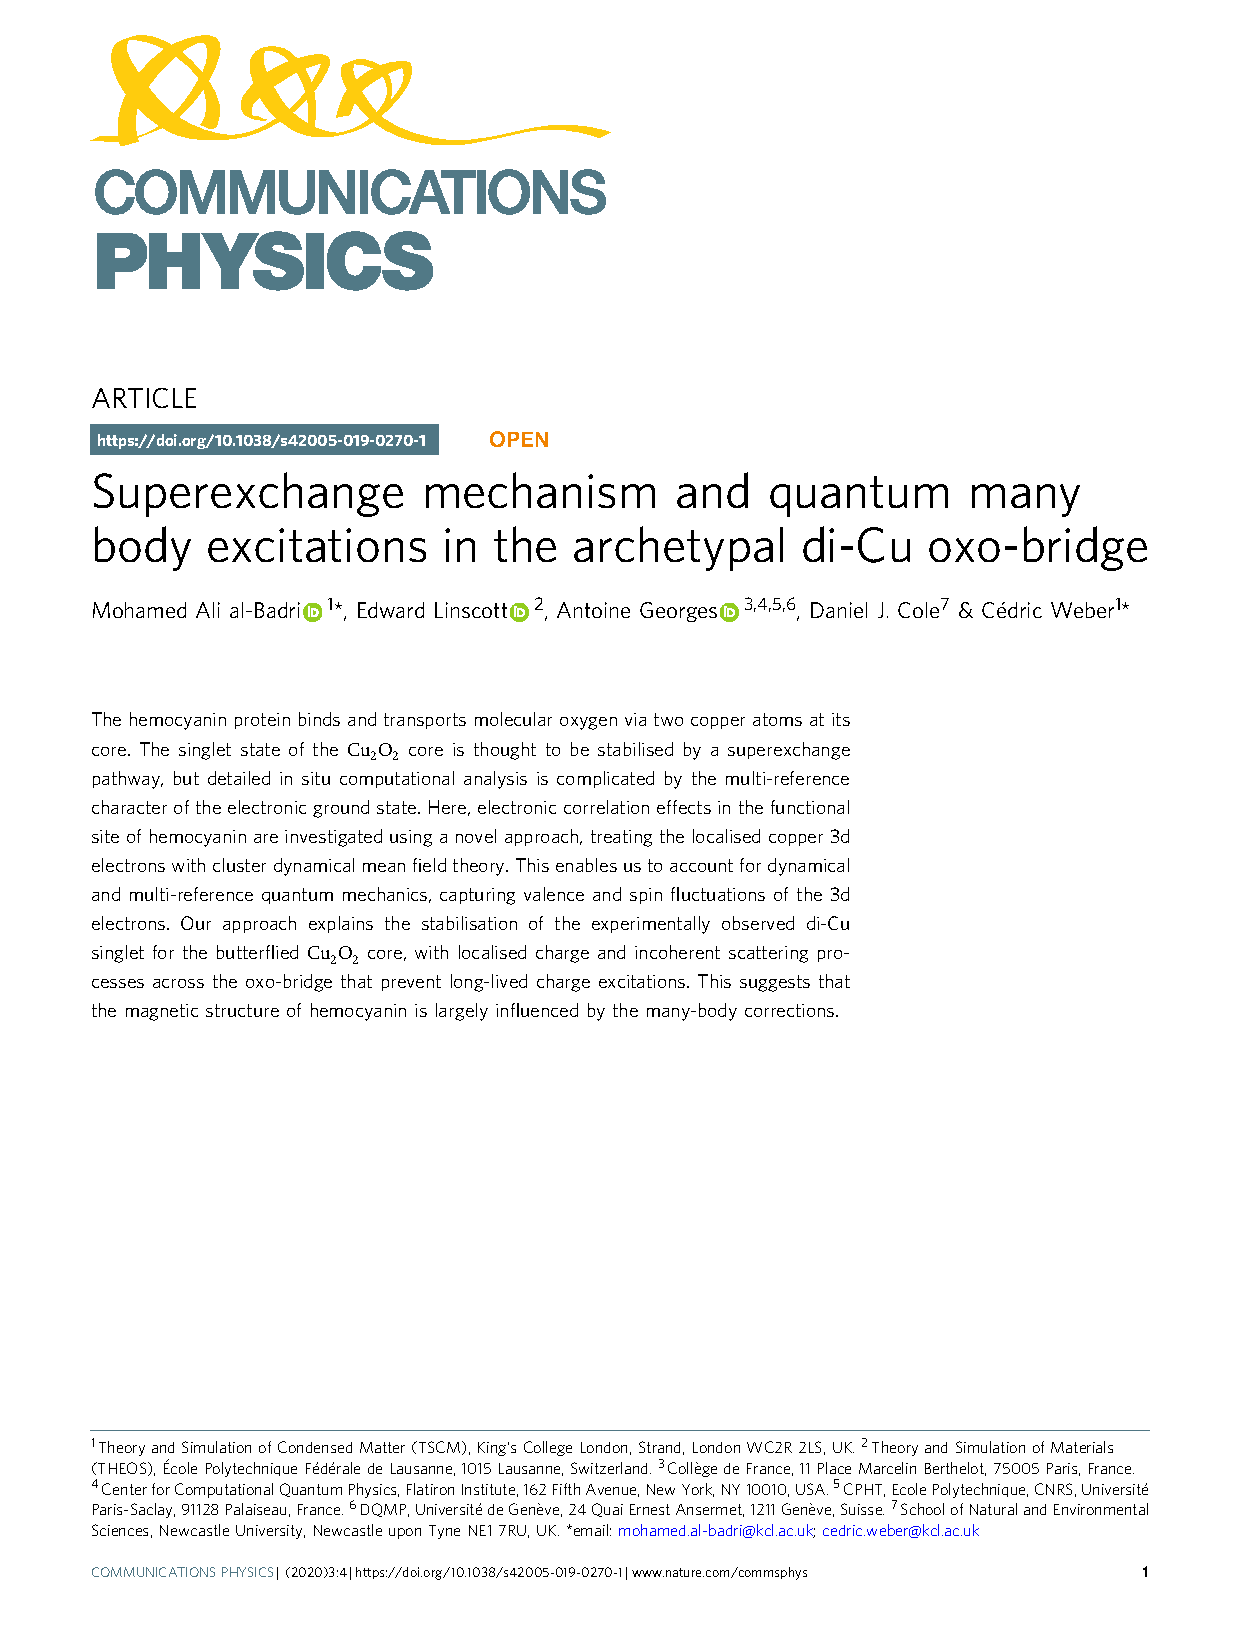
\includepdf[pages=-, offset=75 -75,addtotoc={
     2,section,1,Introduction,pp2,
     2,section,1,Results,pp2,
     2,subsection,2,The spin state of the Cu$_2$O$_2$ core,pp2,
     4,subsection,2,The superexchange mechanism,pp4,
     5,subsection,2,Optical transitions,pp5,
     5,section,1,Discussion,pp5,
     6,section,1,Methods,pp6,
     6,subsection,2,Geometry,pp6,
     6,subsection,2,Density Functional Theory,pp6,
     6,subsection,2,Dynamical Mean Field Theory,pp6},
     addtolist={
     3, figure,{\textbf{The oxyHc functional complex.} Structure showing the Cu$_2$O$_2$ correlated subsystem, which is treated using dynamical mean field theory, and the surrounding imidazole rings representing the protein environment. Hydrogen, carbon, nitrogen, oxygen and iron atoms are shown in white,green, blue, red, and orange respectively.},bb,
     3, figure, {\textbf{The superexchange model of Metz and Solomon.} The Cu$_2$O$_2$ core is depicted from side-on (a,c) and above (b,d). In the planar configuration (a,b), single-ligand orbitals bridge the two copper sites, and superexchange is possible. In a bent configuration (c,d), the copper \textit{d} orbitals overlap with different $\pi^{\ast}$ orbitals. As these two sets of orbitals are orthogonal, hopping between the blue and the red subspaces is not possible and the superexchange mechanism breaks down.},cc,
     4, figure, {\textbf{Decomposition of the reduced density matrix of the Cu$_2$ dimer in the different quantum sectors.} The colours correspond to the respective weights of the different contributions for each value of the Coulomb repulsion $U$ (if a colour occupies all the vertical axis, for example, it means that all eigenvectors of the density matrix are in that particular quantum sector). Note that the $d$ occupation is the sum of both Cu sites (e.g., $d^{20}$ means both Cu atoms are in the $d^{10}$ configuration).},dd,
     4,figure, { \textbf{Dynamical mean field self energy.} a) Imaginary part of the dynamical mean field local self energy $\Sigma(\omega)$ of the Cu-$3d$ empty orbital for Hubbard $U=2$\,eV, $6$\,eV, and $8$\,eV. At $U=8$\,eV, we obtain incoherent excitations at $\omega=0$\,eV. b) The imaginary local self energy at $\omega=0$ and c) the double occupancy of the partially-filled $3d$ orbitals $D$ as a function of $U$. Note that although the double occupancy is evolving smoothly with the Coulomb interaction $U$, $\Sigma(\omega=0)$ shows a sharp increase near $U=8$, associated with the stabilisation of a localised singlet },ee,
     5, figure, { \textbf{Molecular orbital isosurfaces.} The isosurface for the highest occupied molecular orbital (a, c) and lowest unoccupied molecular orbital (b, d) densities for $U = 8$\,eV, as viewed side-on (a, b) and above (c, d). Note that because these are extracted from the Green's function via the spectral density, the phase of the orbitals is inaccessible}, ff,
     5, figure, {\textbf{Theoretical optical absorption of the Cu$_2$O$_2$ core and imidazole rings obtained by dynamical mean field theory for values of the Coulomb repulsion $U=6$ to $10$\,eV.} For comparison, we show the experimental optical absorption in a wide range of wavelengths (infrared to UV). There are several smaller peaks in the experimental spectra that are not visible at this scale (indicated with arrows)}, gg}]{PDF_PAPERS/hemocyanin.pdf}

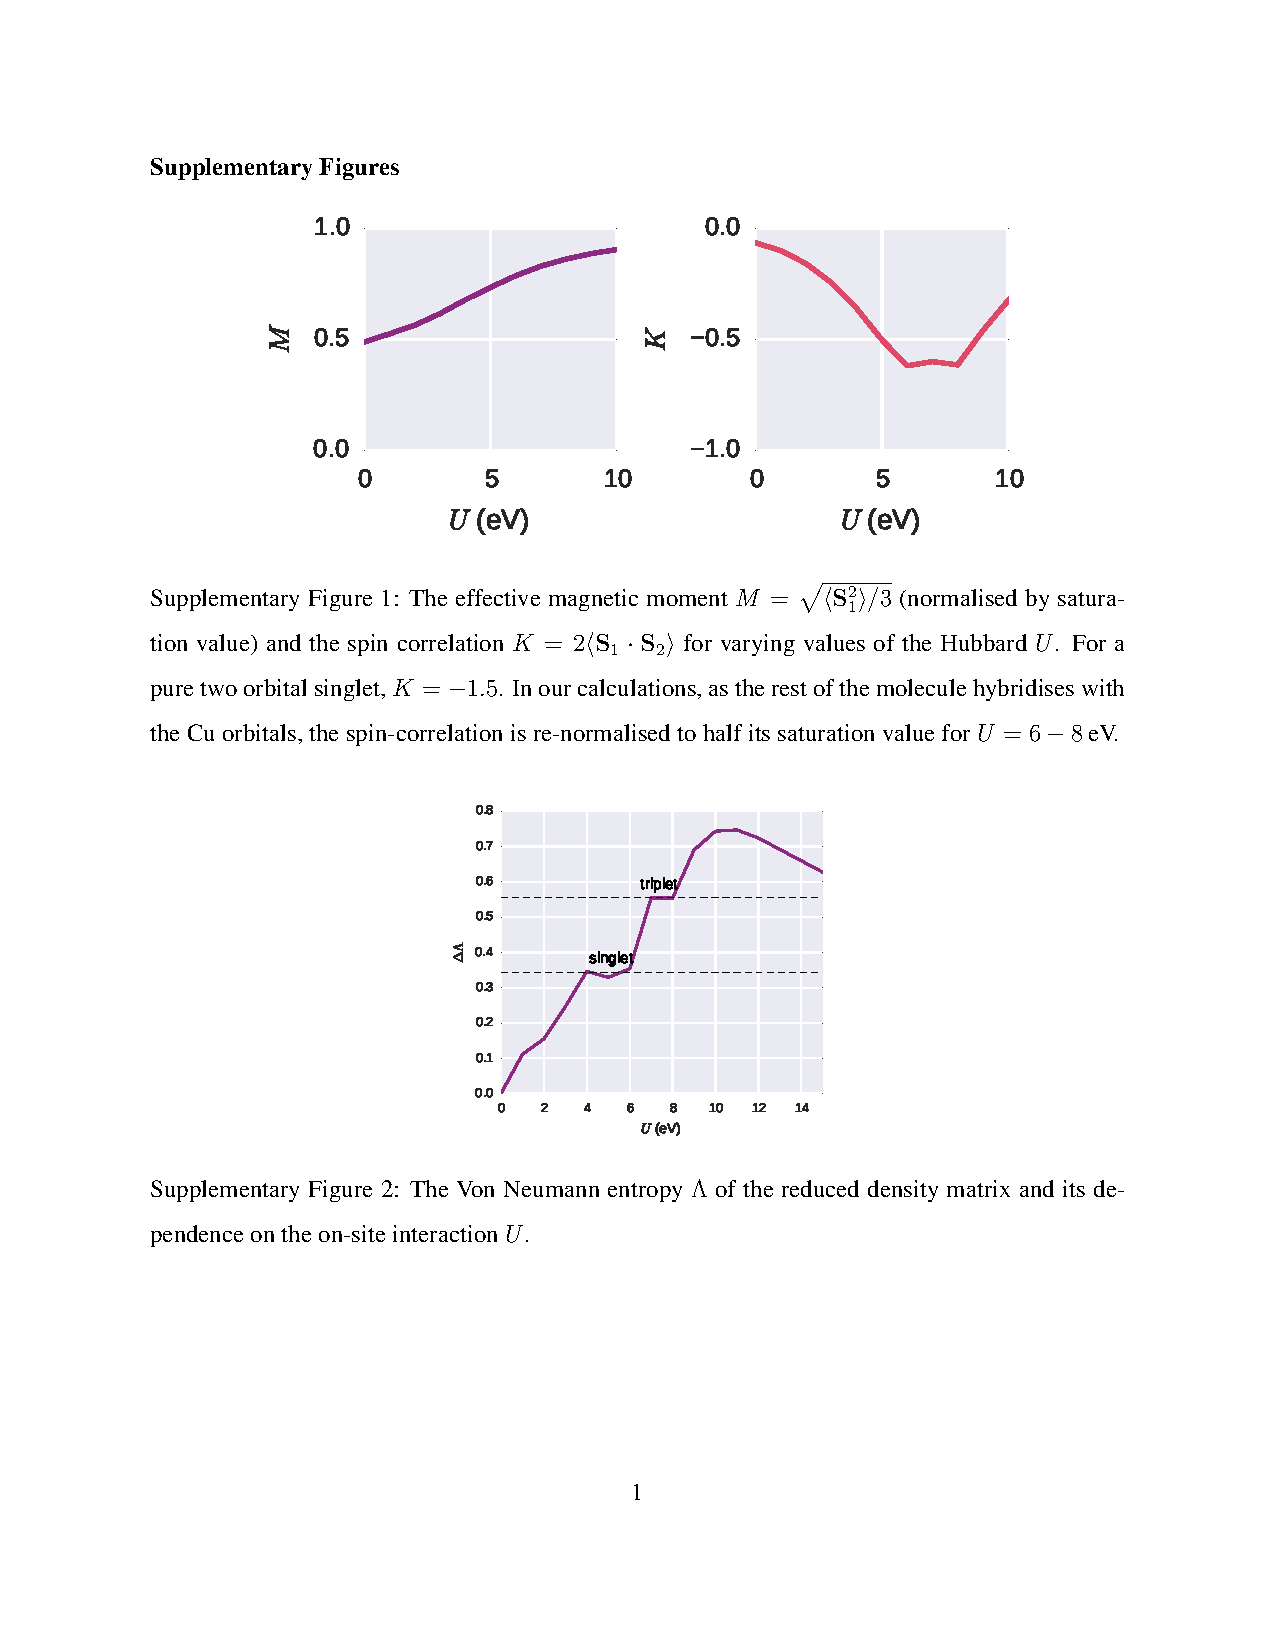
\includepdf[pages=-, offset=75 -75,addtotoc={
     1,section,1,Supplementary Figures,ppp1,
     4,section,1,Supplementary Notes, ppp4,
     4,subsection,2,Details of diamagnetism, ppp4,
     4,subsection,2,Von Neumann entropy, ppp4,
     5,subsection,2,Natural bond orbital analysis, ppp5,
     6,subsection,2,Atomic coordinates of the model system, ppp6,
     8,subsection,2,Convergence of the system-to-AIM mapping,ppp8,
     8,subsection,2,Local axes, ppp8},
     addtolist={
     1, figure,{The effective magnetic moment $M=\sqrt{\langle \mathbf{S}^2_1 \rangle/3}$  (normalised by saturation value) and the spin correlation $K=2\langle \mathbf{S}_1 \cdot \mathbf{S}_2 \rangle$ for varying values of the Hubbard $U$. For a pure two orbital singlet, $K=-1.5$. In our calculations, as the rest of the molecule hybridises with the Cu orbitals, the spin-correlation is re-normalised to half its saturation value for $U=6-8$\,eV.},aaa,
     1, figure,{The Von Neumann entropy $\Lambda$ of the reduced density matrix and its dependence on the on-site interaction $U$.},bbb,
     2, figure,{Isosurfaces of several natural bonding orbitals for $U = 8$\,eV. (a) Two Cu $3d$ orbitals are identified as half-filled by the NBO analysis. (b) The O\textsubscript{2} $\sigma^*$ anti-bond is empty, and does not hybridise with any Cu orbitals. (c) Instead, O $2p$ (blue) to Cu $4s$ (red) charge transfer is favourable.},ccc,
     2,figure,{(a) The local density of states for $U$ = 8\,eV and (b) the different total density of states of the Cu$_2$O$_2$ functional complex for a range of Hubbard $U$ values from DMFT.},ddd,
     3, figure,{The convergence of the distance $d$ as a function of the total number of sites (impurity and bath).}, eee,
     3, figure,{The local axes for the Cu $3d$ correlated subspaces, and the two half-filled NBOs for comparison.}, fff,
     4, table,{The DMFT $3d$ orbital occupations of Cu in our model of ligated hemocyanin for different Hubbard $U$ values, as calculated using NBO. Note that the orbital labels correspond to the local axes to each Cu atom. All eight other Cu $3d$ orbitals had occupancies $> 1.98$ for all values of $U$}, ggg}]{PDF_PAPERS/SI_hemocyanin.pdf}
%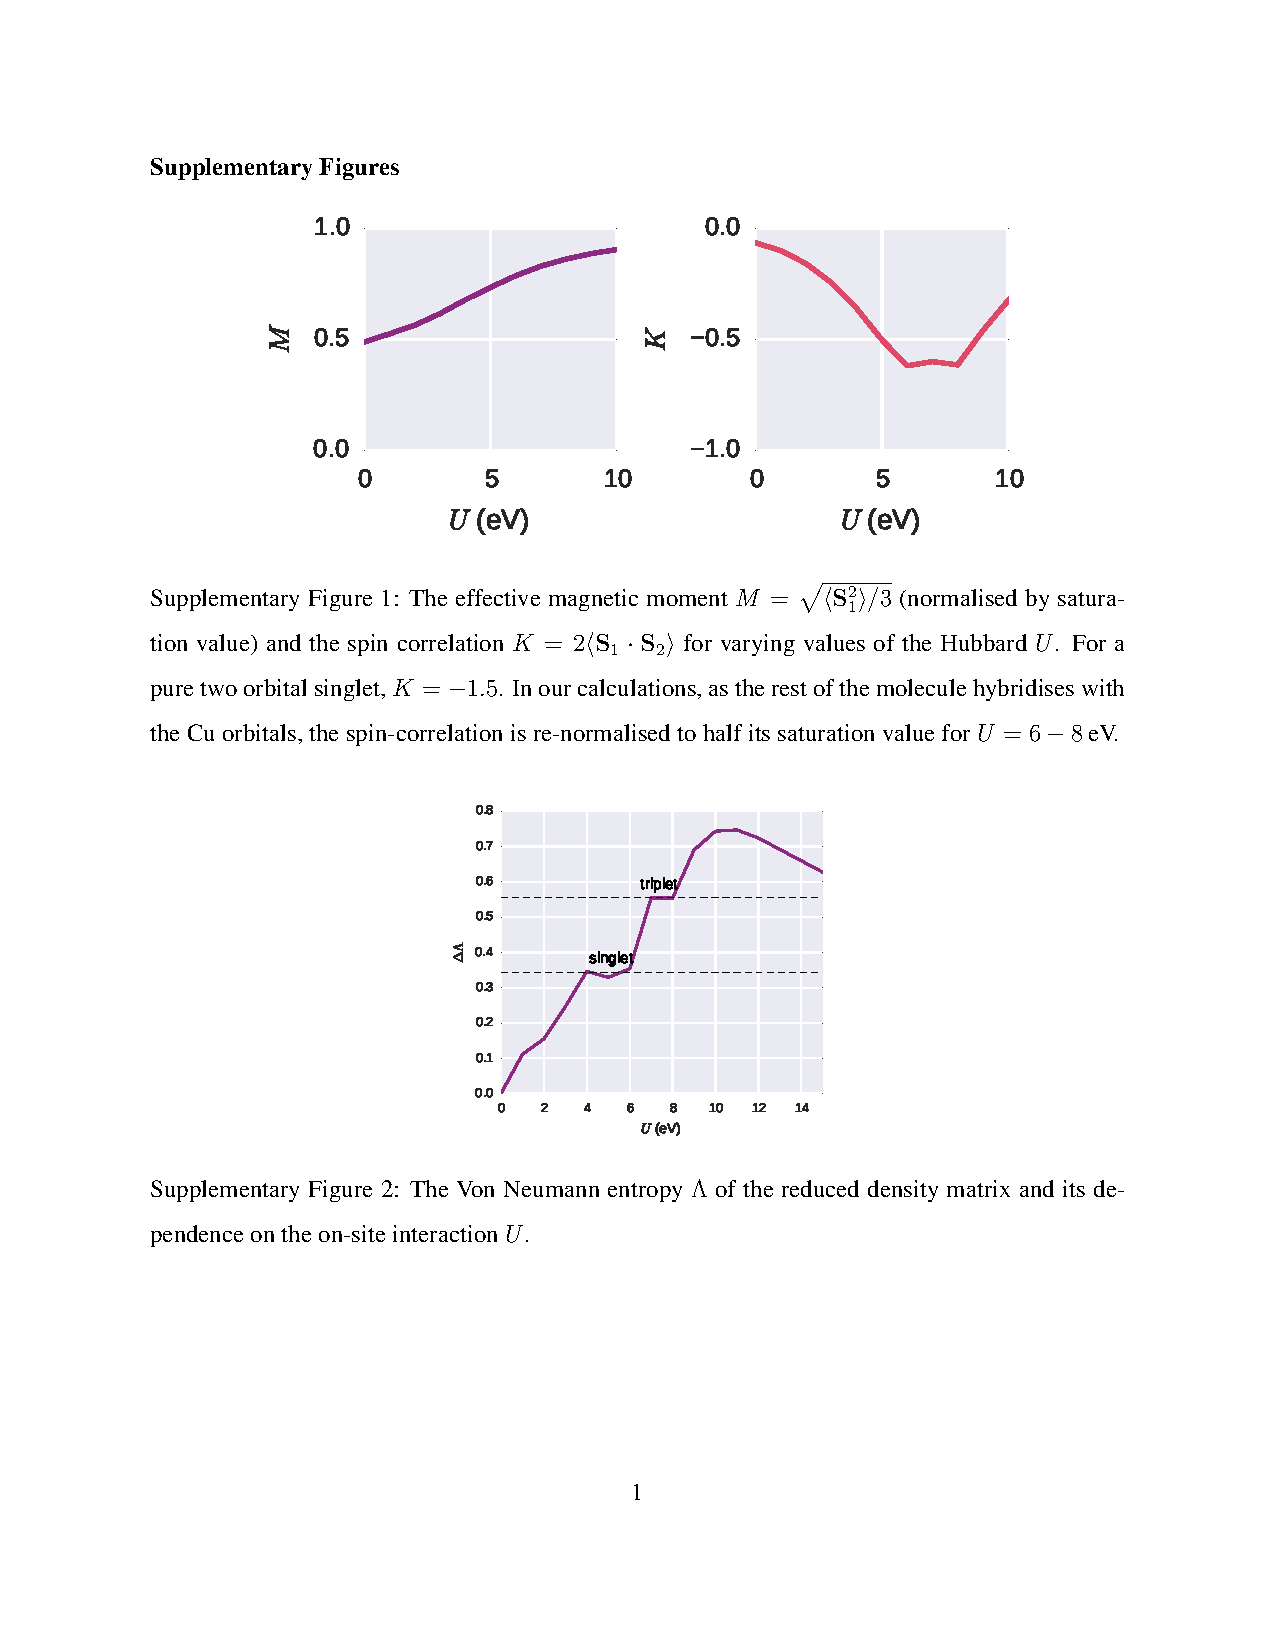
\includepdf[pages=-, offset=75 -75]{PDF_PAPERS/SI_hemocyanin.pdf}




% \chapter{Conclusions}

%\epigraph{\textit{``Nothing more will I teach you today. Clear your mind of questions.”}}{Yoda}
\epigraph{\textit{I am leaving the regions of fact, which are difficult to penetrate, but which bring in their train rich rewards, and entering the regions of speculation, where many roads lie open, but where a few lead to a definite goal.}}{William Ramsay}

Using the methods described throughout this thesis, I have attempted to employ accurate multiscale modelling to address problems within the domain of biology where conventional investigation techniques may be less suitable. This work collectively shows the importance of a multipronged approach to accurate modelling, namely the interdependence of the correct characterisation of structure with the accuracy of the theoretical treatment of a model. \\

I have used density functional theory as a basis to derive a quantum mechanical forcefield for accurate classical molecular dynamics simulations of a graphitic nanomaterial composed of around 1000 atoms. Using this, we investigated the impact of the correlated semi-ordered functionalisation as well as the bespoke forcefield parameters on the nanomaterial's interactions with an ionic solution and its chaotropic potential. This study illustrated the capacity for extrapolating bespoke forcefield parametrisation methods to very large molecular systems, without the need to sacrifice accurate characterisation, which we show is principal to reproducing both experimental and state of the art \textit{ab initio} measurements. Having developed an accurate forcefield model for the system, it is extendable to MD simulations of hundreds of thousands of atoms. \\

Using the accurate structural model of graphitic materials, we used our model to address an open question relating the atomistic interactions at the bio-nano interface. The formation of the protein corona is an obstacle to effectively translating the technological advancements of nanomaterials to biotechnology. The dynamic character of the protein corona has made it a challenging problem to tackle using conventional computational and experimental methods alike. The investigation reported in this thesis utilised numerous analysis techniques to form a collective analysis pipeline to unpick the impact of nano-functionalisation on adsorbed protein structure. Using our results, we were able to make sense of experimentally observed behaviours of the much larger protein corona from a single adsorbed common serum protein. These findings included the way in which some nanomaterial functional groups induce the adsorbed protein to denature its tertiary structure and form binding motifs for protein aggregation; this instigates the formation of a protein corona as observed in experiment. Furthermore, using our analyses we explained the experimentally observed contrast in cellular uptake between different nanomaterial-corona complexes, differing only by functionalisation type. Our analyses showed the impact of conserving functionally important sequences in the protein on the cellular uptake of the nanomaterial-protein complex. Much of the observed behaviour was sensitive to the nanomaterial characterisation, again reinforcing the importance of accurate modelling to associate molecular modelling with experiment.\\

The accurate atomistic modelling of a protein active site, aided by data analysis techniques to unscramble and interpret the dynamics, formed the basis for understanding the role of a catalytic dyad in the function of the SARS-CoV-2 main protease. The protease plays the role of cleaving the viral polyprotein, inhibiting its function therefore disables subsequent viral replication. Unlike the now prevalent preventative immunogenic approaches, protease inhibitors do not require an immunogenic response and can be used to treat both severely afflicted or immunocompromised patients. Unlike many computational approaches to drug discovery, MD simulations clarify the change in dynamics of the protein due to the influencing presence of an inhibitor. Without the previous identification of a potent inhibitor for the similar active site of the SARS-CoV-1 main protease, we would not have been able to unpick the mechanism of the catalytic dyad disruption and use it to calculate the free energy of binding. Since that work was written, the continued efforts to identify protease inhibitors through X-ray crystallography screening have observed numerous ligands that disrupt the His41-Cys145 catalytic dyad. Accelerating the rare-event sampling of the dyad disruption is achieved through the use of Metadynamics simulations, which is completely transferable and open to use by other MD-based projects. This can be used to sample the catalytic dyad disruption within computationally feasible timescales, in order to perform high-throughput screening for as many molecules as possible while retaining the advantages of modelling a dynamic target. \\

The use of electronic structure calculations that account for strong electronic correlations have mostly been reserved for small molecules or periodic systems. We have translated the hybrid DFT+DMFT method to a molecular system to study the active site of the hemocyanin oxygen-transporting protein found in the hemolymph of some invertebrates. It is the first application of cluster DMFT to a biological system, where it identifies the electronic structure of an uncommon open-shell singlet ground state. The singlet ground state is a quantum-entangled superposition of two localised magnetic moments on two distant copper atoms in the hemocyanin active site. This investigation details the function of a superexchange mechanism where electron hopping between the copper $d$-shells is mediated by the bridging dioxygen ligand $p$-orbitals. Its role in reversible oxygen binding is inevitable but is yet to be described using this new information. \\

This work stresses that it is biology that defines the warranted accuracy with which it is to be treated, in line with experimental results to which we return for verifiability. In the pursuit of accuracy, no single theoretical approach can be used to tackle an array of questions aimed at the same class of biomolecular systems. The progress of interdisciplinary collaboration, the advancement of open-source scientific software and increasing experimental data all coalesce into a flourishing environment for collaborative scientific research to advance the multiscale modelling of biomolecular systems and their interface with state-of-the-art nanomaterials. 

\section{Future work}

Having demonstrated the implementation of theoretical approaches to the biological domain in different applications, an extension of this work would build on the most significant divergence from experiment in preexisting methods. The parametrisation of forcefield parameters for graphitic materials is well suited to describing the interfacial properties of a complex chemical environment where strong electrostatic interactions drive the interfacial phenomena. As such, the model could be extended to study the interactions with lipid bilayer systems for which there is abundant demand for multiscale modelling. Furthermore, the availability of linear-scaling electronic structure calculations and forcefield parametrisation software can be used to extend the accuracy to much larger systems in the biological domain. Unlike the predominant application of the interface between biomolecular systems and bespoke forcefield parametrisation of small molecules in the drug discovery domain, the work in this thesis describes its extension to the rapidly growing field of biotechnology. \\

The accurate characterisation and function of the SARS-CoV-2 main protease active site as well as the acceleration of rare-event sampling has been described. This particular work can be extended into an automated pipeline for high-throughput screening of inhibitor ligands. Given the time and computational limitations, this extension remained outside our capacity but nonetheless forms a qualitative proof of principle of how accurate modelling can inform drug delivery efforts for a subset of inhibitor ligands that require the rare-event disruption of the catalytic dyad. \\

The strongly correlated ground state of the hemocyanin active site was resolved using DFT+DMFT and can be extended to other metalloproteins with quantum-mechanically driven biological function. Interestingly, the accurate characterisation of the electronic structure of the hemocyanin active site following this work was extended to bio-mimetic applications in the selective catalytic reduction of nitrogen-oxide pollutants.\cite{chen2019comparative} \\

The field of biotechnology will necessitate the accessible coherent research from both computational and experimental perspectives. Accurate tools are therefore an invaluable requisite for the advancement of the field where the bio-nano interface is concerned. The concomitant advancement of computational architectures and \textit{good} scientific software will improve accessibility to flawlessly research and inform the design of biotechnological solutions. 

%\addcontentsline{toc}{chapter}{Appendices}
\appendix

\chapter{Eigenvalue Distributions of Derivative Operators}
\label{appendix:eigenvalue-distributions}
Using the Circular Diagonalization Theorem \cite{Ingleton1956TheMatrices} one can derive the eigenvalues $\lambda_k$ of an $K\times K$ matrix which represents the second-order central difference approximation to the second derivative on $K$ sites of a one dimensional ring
\begin{align}
	\frac{\partial^2}{\partial x^2} \rightarrow
	\begin{pmatrix}
	  -2 & 1 &  &  &  & 1 \\
	  1 & -2 & 1 &  &  &  \\
	  & 1 & \ddots & \ddots &  & \\
	  & & \ddots & \ddots & 1 & \\
	  & & & 1 & -2 & 1 \\
	  1 & & & & 1 & -2 \\
	\end{pmatrix}\\
	\begin{matrix}
	  \lambda_k =2\left(\cos\left(\frac{2\pi k}{K}\right)-1\right) \\
	  k\in\{0,1,\cdots,K-1\}
	\end{matrix}
	\qquad
\end{align}
As the number of sites $K\rightarrow\infty$ the argument $k/K\in[0,1]$
and the eigenvalues remain bounded $-4<\lambda_k<0$. By shifting and scaling
the index $k\rightarrow\frac{k-K\pi}{2\pi}$ the eigenvalues are expressed as
a dispersion relation
\begin{align}
  \lambda(k)&=
  -2\left(\cos k+1\right)
  \quad k\in[-\pi,\pi]
\end{align}
The discrete $L$-dimensional Laplacian is simply the Kronecker sum $\oplus$ of one
dimensional cases and thus its eigenvalues are simply the sum over one dimensional dispersions \cite{Laub2004MatrixEngineers}
\begin{align}
  \lambda(k)&=
  -2\sum_{i=1}^L\left(\cos k_i+1\right)
  \quad k\in[-\pi,\pi]^L
\end{align}
The probability density $P(\lambda)$ can be expressed as a density integral
over the $L$-dimensional hypercube region $[-\pi,\pi]^L$
\begin{align}
	P(\lambda')&=\frac{1}{Z}\int_{[-\pi,\pi]^L}\!\delta(\lambda'-\lambda(k))\,\mathrm{d}k
\end{align}
We proceed with an element-wise change of variables $u=2\cos k$ and recognise that the integration region is $L$-fold symmetric across each component axis, which allows restriction of the domain of integration to a hyper-octant. In coordinates $u$ the region becomes $[-2,2]^L$
\begin{align*}
  P(\lambda)&=\frac{1}{Z}
  \int_{\Omega'}\!
  \frac{\delta(\Lambda_L+\sum_{i}u_i)}
  {\sqrt{\prod_{i=1}^L(1-u_i^2/4) }}
  \,\mathrm{d}u
  \qquad
  \begin{matrix}
    \Lambda_L=\lambda+2L \\
    |\Lambda_L|\leq2L
  \end{matrix}\\
  &=\frac{1}{2\pi Z}
  \int_{-\infty}^{\infty}\int_{\Omega'}\!
  \frac{\mathbb{e}^{\Lambda_L Ik}\exp[\sum_{i}u_i Ik]}
  {\sqrt{\prod_{i=1}^L(1-u_i^2/4) }}
  \,\mathrm{d}u\mathrm{d}k\\
  &=\frac{1}{2\pi Z}
  \int_{-\infty}^{\infty}\mathbb{e}^{\Lambda_L Ik}
  \prod_{i=1}^L\int_{-2}^{2}\!
  \frac{\mathbb{e}^{u_i Ik}}
  {\sqrt{1-u_i^2/4}}
  \,\mathrm{d}u_i\mathrm{d}k
\end{align*}
The Fourier representation of the delta function allowed the
factorisation of the integral. We recognise a repeated Bessel integral and replace it with the Bessel function of the first kind $J_n(k)$, leaving only a Fourier transform which we define as $\mathcal{F} : f\rightarrow \frac{1}{\sqrt{2\pi}} \int_{-\infty}^{\infty}f(k)e^{ I\Lambda k}\mathrm{d}k$
where
\begin{equation*}
    f(k) = \frac{1}{\sqrt{2\pi}Z}\prod_{i=1}^L\int_{-2}^{2}\!
  \frac{\mathbb{e}^{u_i Ik}}
  {\sqrt{1-u_i^2/4}} \mathrm{d}u_i
\end{equation*}
To clean the formula up even further we may use the convolution theorem to deal with the powers of $L$, leaving only the Fourier transform of the Bessel function $J_0(k)$, which is the arcsine distribution $\alpha(\lambda)$. The eigenvalue density of a Kronecker sum of matrices is the convolution of the densities of those matrices.
\begin{align}
  P(\lambda)=\underbrace{
  \alpha(\lambda)*\alpha(\lambda)*\cdots*\alpha(\lambda)}_{L}\qquad\qquad\label{eq:mlap}\\
    \alpha(\lambda)=
      \frac{\Pi\left(\frac{\lambda+2}{2}\right)}{2\pi\sqrt{1-\left(\frac{\lambda+2}{2}\right)^2}}
    \qquad
    \Pi(x)=
      \begin{cases}
        1 & |x|<1\\
        0 & |x|\geq1\\
      \end{cases}
	\label{eq:laplacian-distribution}
\end{align}
\begin{Figure}
    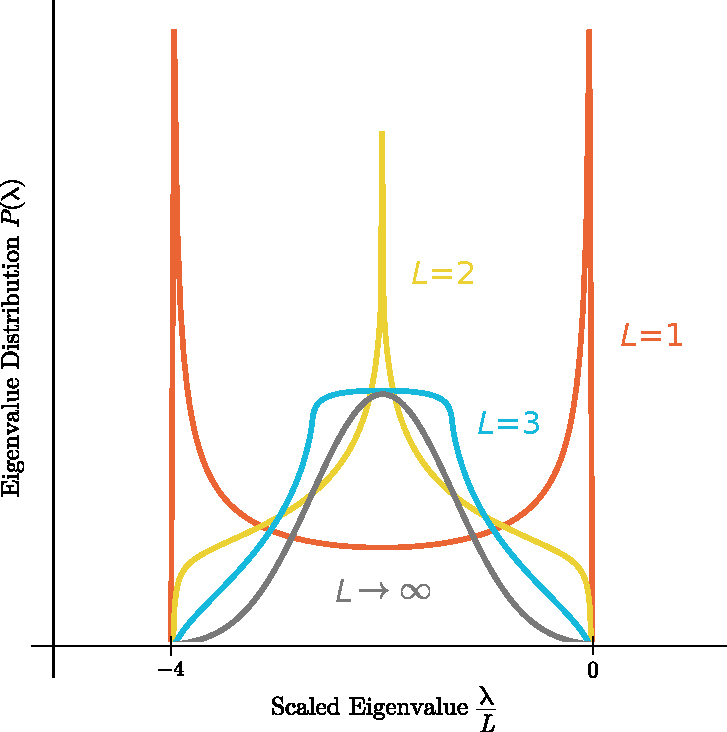
\includegraphics[width=0.6\linewidth]{laplacian-spectra}
    \caption{Eigenvalue distributions $P(\lambda)$ of the $L$-dimensional Laplacian}
    \label{fig:laplacian-spectra}
\end{Figure}
The one dimensional density has two Van Hove singularities at $\lambda=-4,0$ given by the arcsine law $\alpha(\lambda)$, whereas the two dimensional case has one at $\lambda=-4$ given by the complete elliptic integral of the first kind $K(m)$. Figure \ref{fig:laplacian-spectra} reveals that in higher dimensions singularities do not occur; instead there appear to be discontinuities in the higher order derivatives. The density smooths out as repeated convolutions bring it to a normal distribution; this is another way to state the Central Limit Theorem. In the context of diffusion, the Laplacian is scaled by the diagonal diffusion matrix. To take this scaling into account, components $D_i$ are introduced in the arcsine laws
\begin{align}
	\alpha(\lambda) \rightarrow \frac{1}{D_i}\alpha(\lambda/D_i)
\end{align}
The eigenvalue distributions determine the eigenbasis evolution  \eqref{eq:eigenbasis-vector-evolution} which reveals that the second order derivative leads to exponential relaxation of all basis vectors, except for the subset with vanishing eigenvalue $\lambda=0$. The corresponding zero eigenvectors $v_0$ are the Fourier components of the steady state distribution, and are the only components that remain as $t\rightarrow\infty$. The diffusive components $D_i$ determine the timescale of relaxation in each dimension.


\chapter{Interpretation of Morphogen Gradients by a Bistable Circuit}
\label{appendix:double-exclusive}
\includepdf[pages=1-51, offset=75 -90, scale=0.85, frame,
        clip,trim=20mm 5mm 20mm 15mm,
        pagecommand={}, addtotoc={
                2,section,1,Supplementary Figures,appendix:double-exclusive:figures,
                18,section,1,Supplementary Methods,appendix:double-exclusive:methods,
                19,subsection,2,Differential Equation Models \& Parameter Inference,appendix:double-exclusive:inference,
                40,subsection,2,Bistability Analysis,appendix:double-exclusive:bistability,
                42,subsection,2,Boundary Experiments,appendix:double-exclusive:boundaries,
                50,subsection,2,Models of the Exclusive Receiver Relay Circuits,appendix:double-exclusive:relay},
        addtolist={
                2, figure, {\textit{Supplementary Figure 1}\quad Circuit variants}, fig:double-exclusive:variants,
                4, figure, {\textit{Supplementary Figure 2}\quad Raw timecourse fluorescence traces}, fig:double-exclusive:plate-data,
                15, figure, {\textit{Supplementary Figure 13}\quad Hysteresis flow cytometry experiments}, fig:double-exclusive:flow-hysteresis,
                41, figure, {\textit{Supplementary Figure 25}\quad Bifurcation curves for uniform and protected degradation models}, fig:double-exclusive:degradation-models,
                41, figure, {\textit{Supplementary Figure 26}\quad Bifurcation curve insensitivity specific growth rate $\gamma_0$}, fig:double-exclusive:growth-rate-sensitivity
}]{publications/double-exclusive-si.pdf}

\chapter{Parameter Inference with Bifurcation Diagrams}
\label{appendix:inference}
\includepdf[pages=1-6, offset=75 -90, scale=0.85, frame,
        clip,trim=33mm 20mm 33mm 20mm,
        pagecommand={}, addtotoc={
                1,section,1,Bifurcation Diagrams as Tangent Fields,appendix:tangent-fields,
                2,section,1,Bifurcation Measure Properties,appendix:bifurcation-measure,
                3,section,1,Leibniz Rule for Space Curves,appendix:leibniz-rule,
                5,section,1,Application to the Double Exclusive Model,appendix:more-complex-model,
                6,section,1,Extension for Hopf Bifurcations,appendix:hopf-measure},
        addtolist={
                1, figure, {\textit{Supplementary Figure 1}\quad Two implicit surfaces $f_{\theta}(z)=0$ and $g_{\theta}(z)=0$ in $\mathbb{R}^3$ intersecting to form a space curve which is tangent to field $\tangent(z)$ and perpendicular to gradients $\partial_{z}f_{\theta}$ and $\partial_{z}g_{\theta}$}, fig:implicit-surfaces,
                2, figure, {\textit{Supplementary Figure 2}\quad Left/Right : Determinant $\Det$ and tangent field $\tangent(z)$ for the saddle-node/pitchfork models for some set values of $\theta$ revealing that $\Det=0$ defines bifurcations}, fig:determinant-field,
                5, figure, {\textit{Supplementary Figure 3}\quad Bifurcation inference for the \emph{double exclusive reporter}. A. Optimal parameter estimates $\theta^*$ for the targets $\targets=\{1,2\}$ (indicated by yellow lines in panel B) reveal four regions  with two geometrically different regimes: mutual activation (region 1) and mutual inhibition (regions 2-4). B. Example bifurcation diagrams indicate that region 2 has swapped kinetics between $L$ and $T$ to region 3. Region 4 has models with non-zero imaginary parts to eigenvalues indicating damped oscillations (shown in light green).},
                fig:double-exclusive-optima,
                6, figure, {\textit{Supplementary Figure 4}\quad Bifurcation measure $\measure(s)$ and eigenvalues $\lambda(s)$ along the arclength $s$ for two different bifurcation curves demonstrating how the measure detects non-zero imaginary parts $\Imag[\lambda]$ (onset of damped oscillations marked by circle) and sign changes in real parts $\Real[\lambda]$ (Hopf bifurcations marked by stars)},
                fig:hopf-measure
}]{publications/bifurcation-inference-si.pdf}

\chapter{Exploring Bifurcations between Phenotypes}
\label{appendix:exploring}

\section{Experimental Methods}
\subsection{Tissue Acquisition \& Dissociation} 

All samples were collected via the \href{https://www.cbtm.group.cam.ac.uk}{Cambridge Biorepository for Translational Medicine} under Research Ethics Committee approval 15/EE/0152. Tissue was obtained from five deceased organ donors following circulatory death. Donor metadata is given in Table \ref{table:donors}. Briefly, following cessation of circulatory function donors proceeded to organ donation. Organs were perfused \emph{in situ} with cold organ preservation solution and cooled with topical application of ice. Samples for the study were obtained within 60 minutes of cessation of circulation and placed in University of Wisconsin organ preservation solution for transport at 4°C to the laboratory. Lung and liver samples were obtained from the left lower lobe of the lung and the right lobe of the liver. In addition, two donor-matched blood samples were collected prior to withdrawal of life support, under approval 97/290.

To minimise the possibility of processing-depended differences in cell surface marker expression, all samples, including blood, were processed using enzymatic digestion protocol. Briefly, solid tissues were weighed, transferred into 10cm tissue culture dishes and cut into small pieces. Up to 5g of tissue was then transferred to each of eight GentleMACS C tubes (Miltenyi Biotec) containing 5mL of dissociation media composed of X-vivo15 supplemented with 0.13U/mL Liberase TL (Roche), 10U/mL Benzonase nuclease (Millipore/Merck), 2\% (v/v) heat-inactivated fetal bovine serum (FBS, Gibco), penicillin (100 U/ml, Sigma-Aldrich), streptomycin (0.1 mg/ml, Sigma-Aldrich), and 10mM HEPES (Sigma Aldrich). The samples were then dissociated on a GentleMACS Octo dissociator (Miltenyi Biotec) running a protocol that provided gradual ramping up of homogenisation speed and two 15 minute heating/mixing steps at 37°C. Digested tissue was passed through a 70$\mu$m MACS Smartstrainer (Miltenyi Biotec) and the flow-through was first washed with media supplemented with 2 mM EDTA and then with PBS. Mononuclear cells were enriched by Ficoll-Paque (GE Healthcare) density centrifugation according to manufacturer's instructions. Following, density centrifugation, mononuclear layer was collected, washed once with PBS and cell pellet was resuspended in FACS buffer (PBS, 2.5$\%$ FBS).

Bone marrow aspirates and peripheral blood samples were first subjected to Ficoll-Paque density centrifugation, according to manufacturer's instructions, the mononuclear layer was then collected, washed with PBS and cells were treated with the same dissociation media as solid tissues for 30 min at 37°C prior to washing and resuspension in FACS buffer.

\subsection{Flow Cytometry}

Depending on the cell yield, up to 1x10\textsuperscript{6} mononuclear cells/tissue were stained with antibodies shown in Table \ref{table:panel}. Not all donors were stained with the same panel. To expand total number of markers, sentinel panel design was implemented where CD3 and IgD were detected with antibodies conjugated to BUV395 and Foxp3 and IgM were detected with antibodies conjugated to PE in some donors. Refer to Table \ref{table:panels} for details. 

Single cell suspensions were washed once in PBS, transferred into 96 v-bottom plate and stained with Zombie UV viability dye for 30 min at 4°C following by a wash with FACS buffer. Cell pellets were resuspended in 50$\mu$l FACS buffer with Human FcR block (BD Biosciences) and incubated for 10 min at 4°C. Next, cells were pelleted, excess buffer removed and 100$\mu$l of antibody master mix composed of cell-surface antibody cocktail (see Table \ref{table:panels}), BV buffer (BD) and True-Stain Monocyte Blocker (Biolegend) and incubated for 1h at 4°C. Following incubation, cells were washed three times in PBS and prepared for intracellular staining using transcription factor fixation/permeabilisation kit (eBioscience) according to the manufacturer's instructions. Following IC staining, cell were resuspended in PBS and analysed on BD FACSymphony A3 cell analyser within 10 hours.

\section{Supplementary Tables}

\begin{landscape}
\begin{table}
\footnotesize
\begin{center}
\begin{tabular}{>{\centering\arraybackslash}p{0.6cm}>{\centering\arraybackslash}p{0.4cm}>{\centering\arraybackslash}p{0.7cm}>{\centering\arraybackslash}p{0.9cm}>{\centering\arraybackslash}p{0.9cm}>{\centering\arraybackslash}p{0.9cm}>{\centering\arraybackslash}p{1cm}>{\centering\arraybackslash}p{1cm}>{\centering\arraybackslash}p{1cm}>{\centering\arraybackslash}p{1cm}>{\centering\arraybackslash}p{2.1cm}>{\centering\arraybackslash}p{0.6cm}}
    \toprule
    Donor ID & Sex & Age & Primary cause of death & Multi-trauma & Days in hospital & BMI &CMV/ EBV/ TOXO& Smoking & Alcohol (u/day) & Antibiotics within 2 weeks of death & Steroids \\
    \midrule
    390C & F & 65-70 & ICH & \cmark & 2 & 30-35 & $+$/$+$/$-$ & ? & $<$1 & \xmark & \xmark \\
    403C & M & 50-55 & ICH & \cmark & 8 & 30-35 & $+$/$+$/$-$ & \cmark & $<$1 & Co, T & \xmark \\
    423C & M & 60-65 & ICH & \xmark & 2 & 20-25 & $-$/$+$/$-$ & \cmark & $>$9 & G, F & D \\
    412C & M & 70-75 & ICH & \xmark & 5 & 26-30 & $-$/$+$/$+$ & \cmark & $<$2 & A$^\star$ , F, G, C, Co & P$^\dagger$ \\
    428C & F  & 55-60 & ICH & \xmark & 3 & 20-25 & $-$/$+$/$-$ & \cmark & $>$9 & Co & \xmark \\
    \bottomrule
\multicolumn{12}{p{\linewidth}}{\vline height10pt width0pt
\relax F = Female; M = Male; ICH = intracranial haemorrhage; CMV = Cytomegalovirus; EBV = Epstein-Barr virus; TOXO = Toxoplasmosis; Co = Co-amoxiclav; A = Amoxicillin; T = Tazocin; F = Flucloxacillin; G = Gentamicin; D = Dexamethasone; C = Clarithromycin; \cmark = Yes; \xmark = No; ? = Not known;P = Prednisolone; $^\star$pre-admission, $^\dagger$pre-treatment}\\
\end{tabular}
\caption{Donor Metadata}
\label{table:donors}
\end{center}
\end{table}
\end{landscape}

\begin{table}
\footnotesize
\begin{center}
    \begin{tabular}{llll}
        \toprule
        Specificity & Fluorochrome & Clone & Source \\
        \midrule
        CD3 &  BUV395 & SK7 & BD \\
        CD8 & BUV563 & RPA-T8 & BD \\
        CD69 & BUV737 & FN50 & BD \\
        CD4 & BUV805 & SK3 & BD \\
        CD4 & BUV661 & SK3 & BD \\
        CD45 & BUV805 & HI30 & BD \\
        CD103 & BV421 & Ber-ACT8 & BD \\
        HLA-DR & BV510 & G46-6 & BD \\
        CD127 & PE-Cy7 & HIL-7R-M21 & BD \\
        CCR4 & BV605 & L291H4 & Biolegend \\
        CCR6 & BV650 & 11A9 & BD \\
        PD-1 & BV711 & EH12.1 & BD \\
        CD45RA & BV786 & HI100 & BD \\
        CCR10 & BB515 & 1B5 & BD \\
        CXCR3 & BB700 & 1C6/CXCR3 & BD \\
        CXCR5 & APC-R700 & RF8B2 & BD \\
        CCR7 & APC-Fire750 & G043H7 & Biolegend \\
        CD25 & APC & M-A251 & BD \\
        CD25 & APC & 2A3 & BD \\
        CD19 & BV570 & HIB19 & Biolegend \\
        IgM & PE & G20-127 & BD \\
        IgD & BUV395 & IA6-2 & BD \\
        Foxp3 & PE & 269D/C7 & BD \\
        Foxp3 & PE & PCH101 & eBioscience \\
        Helios & PE-Dazzle & 22F6 & Biolegend \\
        Zombie UV & - & - & Biologend \\
        \bottomrule
    \end{tabular}
\caption{Details of antibodies used in this study}
\label{table:panel}
\end{center}
\end{table}

\begin{table}
\footnotesize
\begin{center}
    \begin{tabular}{lrlll}
        \toprule
        & \multicolumn{4}{c}{Fluorochromes} \\
        \cmidrule{3-5}
         & Panels:&  A &  B &  C \\
        \cmidrule{3-5}
        Specificity & Donor:& 390C & 403C & 412C, 423C, 428C \\
        \midrule
        CD45 && BUV805 & - & - \\
        CD19 && - & - & BV570 \\
        IgM && - & - & PE \\
        IgD && - & - & BUV395 \\
        CD4 && \textbf{BUV661} & \textbf{BV805} & \textbf{BV805} \\
        CD3 &&  BUV395 & BUV395 & BUV395 \\
        CD8 && BUV563 & BUV563 & BUV563 \\
        CD69 && BUV737 & BUV737 & BUV737 \\
        CD103 && BV421 & BV421 & BV421 \\
        HLA-DR && BV510 & BV510 & BV510 \\
        CD127 && PE-Cy7 & PE-Cy7 & PE-Cy7 \\
        CCR4 && BV605 & BV605 & BV605 \\
        CCR6 && BV650 & BV650 & BV650 \\
        PD-1 && BV711 & BV711 & BV711 \\
        CD45RA && BV786 & BV786 & BV786 \\
        CCR10 && BB515 & BB515 & BB515 \\
        CXCR3 && BB700 & BB700 & BB700 \\
        CXCR5 && APC-R700 & APC-R700 & APC-R700 \\
        CCR7 && APC-Fire750 & APC-Fire750 & APC-Fire750 \\
        CD25 && APC & APC & APC \\
        Foxp3 && PE & PE & PE \\
        Helios && PE-Dazzle & PE-Dazzle & PE-Dazzle \\
        Zombie UV && Zombie UV & Zombie UV & Zombie UV \\
        \bottomrule
    \end{tabular}
\caption{Immunophenotyping panel designs used in the dataset}
\label{table:panels}
\end{center}
\end{table} 
% You could separate these out into different files if you have
%  particularly large appendices.

% This line manually adds the Bibliography to the table of contents.
% The fact that \include is the last thing before this ensures that it
% is on a clear page, and adding it like this means that it doesn't
% get a chapter or appendix number.
\addcontentsline{toc}{chapter}{Bibliography}
% Actually generates your bibliography.
\bibliography{biblio}

% All done. \o/
\end{document}
